%% Dokumentklasse KOMA-Script Report
\documentclass[paper=a4, 12pt, twoside]{scrreprt}
%% Einrückung des Inhaltsverzeichnis ändern!
\makeatletter 
\renewcommand*\l@section{\bprot@dottedtocline{1}{1em}{2em}} % Original 1.5 und 2.3 
\renewcommand*\l@subsection{\bprot@dottedtocline{2}{1.5em}{2.8em}} % Original 3.8 und 3.2 
\makeatother
% report zweiseitig gemacht!
%% Encoding UTF8
\usepackage[utf8]{inputenc}
%% 8 Bit Aufloesung der Buchstaben
\usepackage[T1]{fontenc}
%% Seitenraender
\usepackage[scale=0.72]{geometry}
%% Spracheinstellungen
\usepackage[english, naustrian]{babel} % your native language must be the last one!!
%% erweiterte Farbenpalette
\usepackage[dvipsnames]{xcolor}
%% Abbildungen
\usepackage{graphicx}
%% Tabellen (erweitert)
\usepackage{tabularx}
%% TikZ + Circuit-TikZ (fuer Schaltungen)
\usepackage[europeanresistors, europeaninductors]{circuitikz}
%% Nuetzliche TikZ Libraries
\usetikzlibrary{arrows, automata, positioning}
%% mathematik
\usepackage{amsmath, amssymb}
%\usepackage{mathtools}	
%% pdf-einbindung
\usepackage{pdfpages}
%% scource-code einbindung
\usepackage{listings, scrhack} %scrhack vermeidet Umschaltung auf KOMA Floats..
\usepackage{courier}
%% euro-symbol
\usepackage{eurosym}
%% landcsape-seiten ermöglichen
\usepackage{lscape}

%% Diplomarbeits-Format
\usepackage{srdpdipa}

%% Abkuerzungsverzeichnis
\usepackage[]{acronym}

%% Todos
\usepackage[]{todonotes}

%% Ganttdiagramme
\usepackage{pgfgantt}

%% Subfigures
\usepackage[lofdepth]{subfig}

%% Quotes
\usepackage{csquotes}

%%Comments
\usepackage{comment}
\excludecomment{comment}

%% Für figures (H)
\usepackage{float}

%% Bei Bildern für valign
\usepackage[export]{adjustbox}

%% Für Tabellen
\usepackage{tabularx}
\usepackage{multirow}

\usepackage[justification=centering]{caption}

%% PDF
\usepackage{pdfpages} 

\usepackage{graphicx} 
\usepackage{textcomp}

%% Figuren drehen
\usepackage{rotating}
\usepackage{tikz}

%% definitionen =====================================%%
\dataSchool{HTBLuVA St. Pölten}
\dataDepartment{Höhere Lehranstalt für Elektronik und Technische Informatik}
\dataSubdepartment{Ausbildungsschwerpunkte Embedded- \& Wireless Systems}
\dataSession{2016/17}

\title{Bluetooth-Aktivbox}
\author{Markus Bointner \and Andreas Macsek}
\date{\today}
\place{St. P\"olten}
\professor{Prof. Dipl.-Ing. Dr. Herbert Wagner}
%%====================================================%%

% Hyperlinks im Dokument
\usepackage[colorlinks=true,
    linkcolor=black,
    citecolor=green,
    bookmarks=true,
    urlcolor=black,
    bookmarksopen=true]{hyperref}

\begin{document}

%% Richtige Einrückung für doppelseitiges Format (Auf der Innenseite mehr Abstand)
\oddsidemargin10mm
\evensidemargin0mm

\frontmatter

%% titelseite ==========================================%%
\maketitle
%%======================================================%%

%% komplett leere seite ================================%%
\newpage\null\thispagestyle{empty}%\newpage
%%======================================================%%

%% eidesstattliche erklärung ===========================%%
\begin{affidavit}
    \unterschrift{Markus Bointner}
    \unterschrift{Andreas Macsek}
\end{affidavit}
%%======================================================%%

%% dokumentation (deutsch/englisch) ====================%%
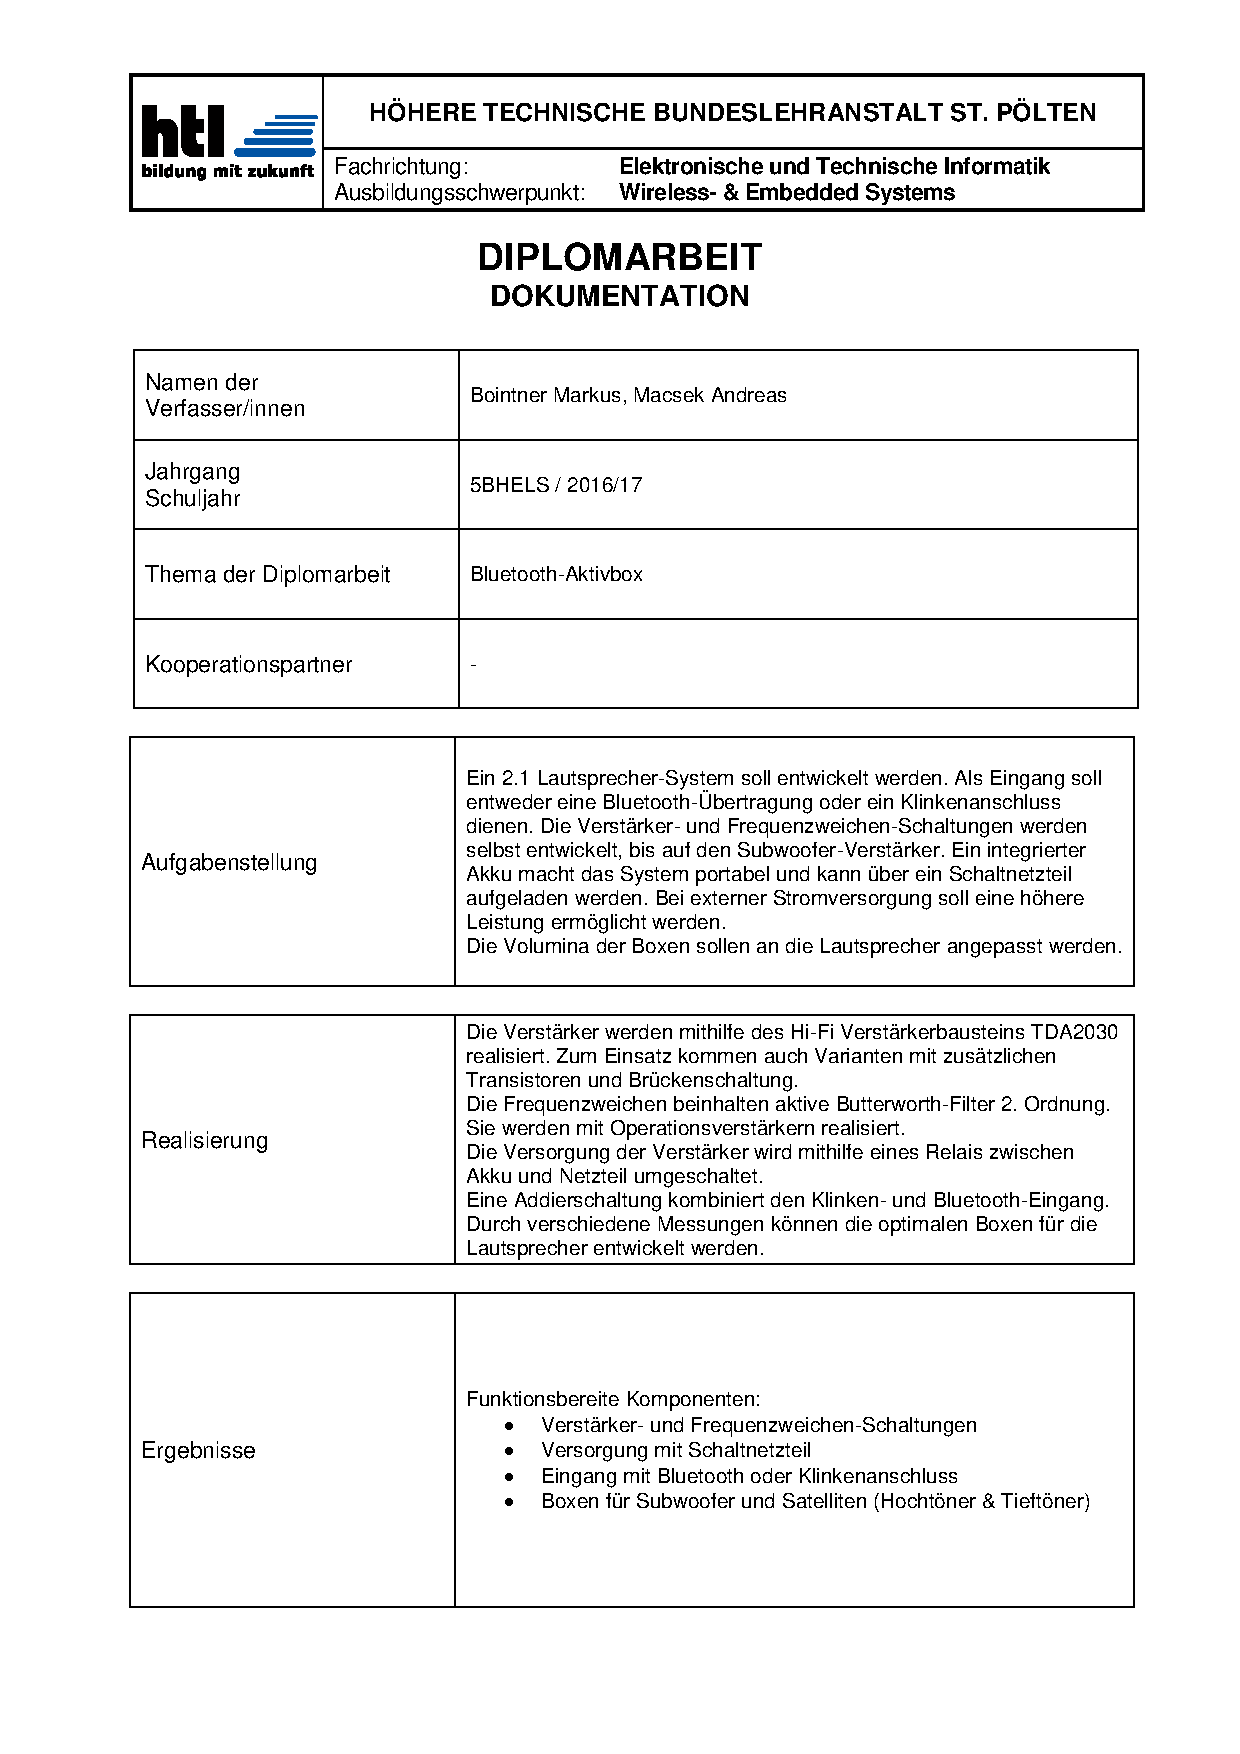
\includepdf[pages=-]{form/dokumentation-de.pdf}
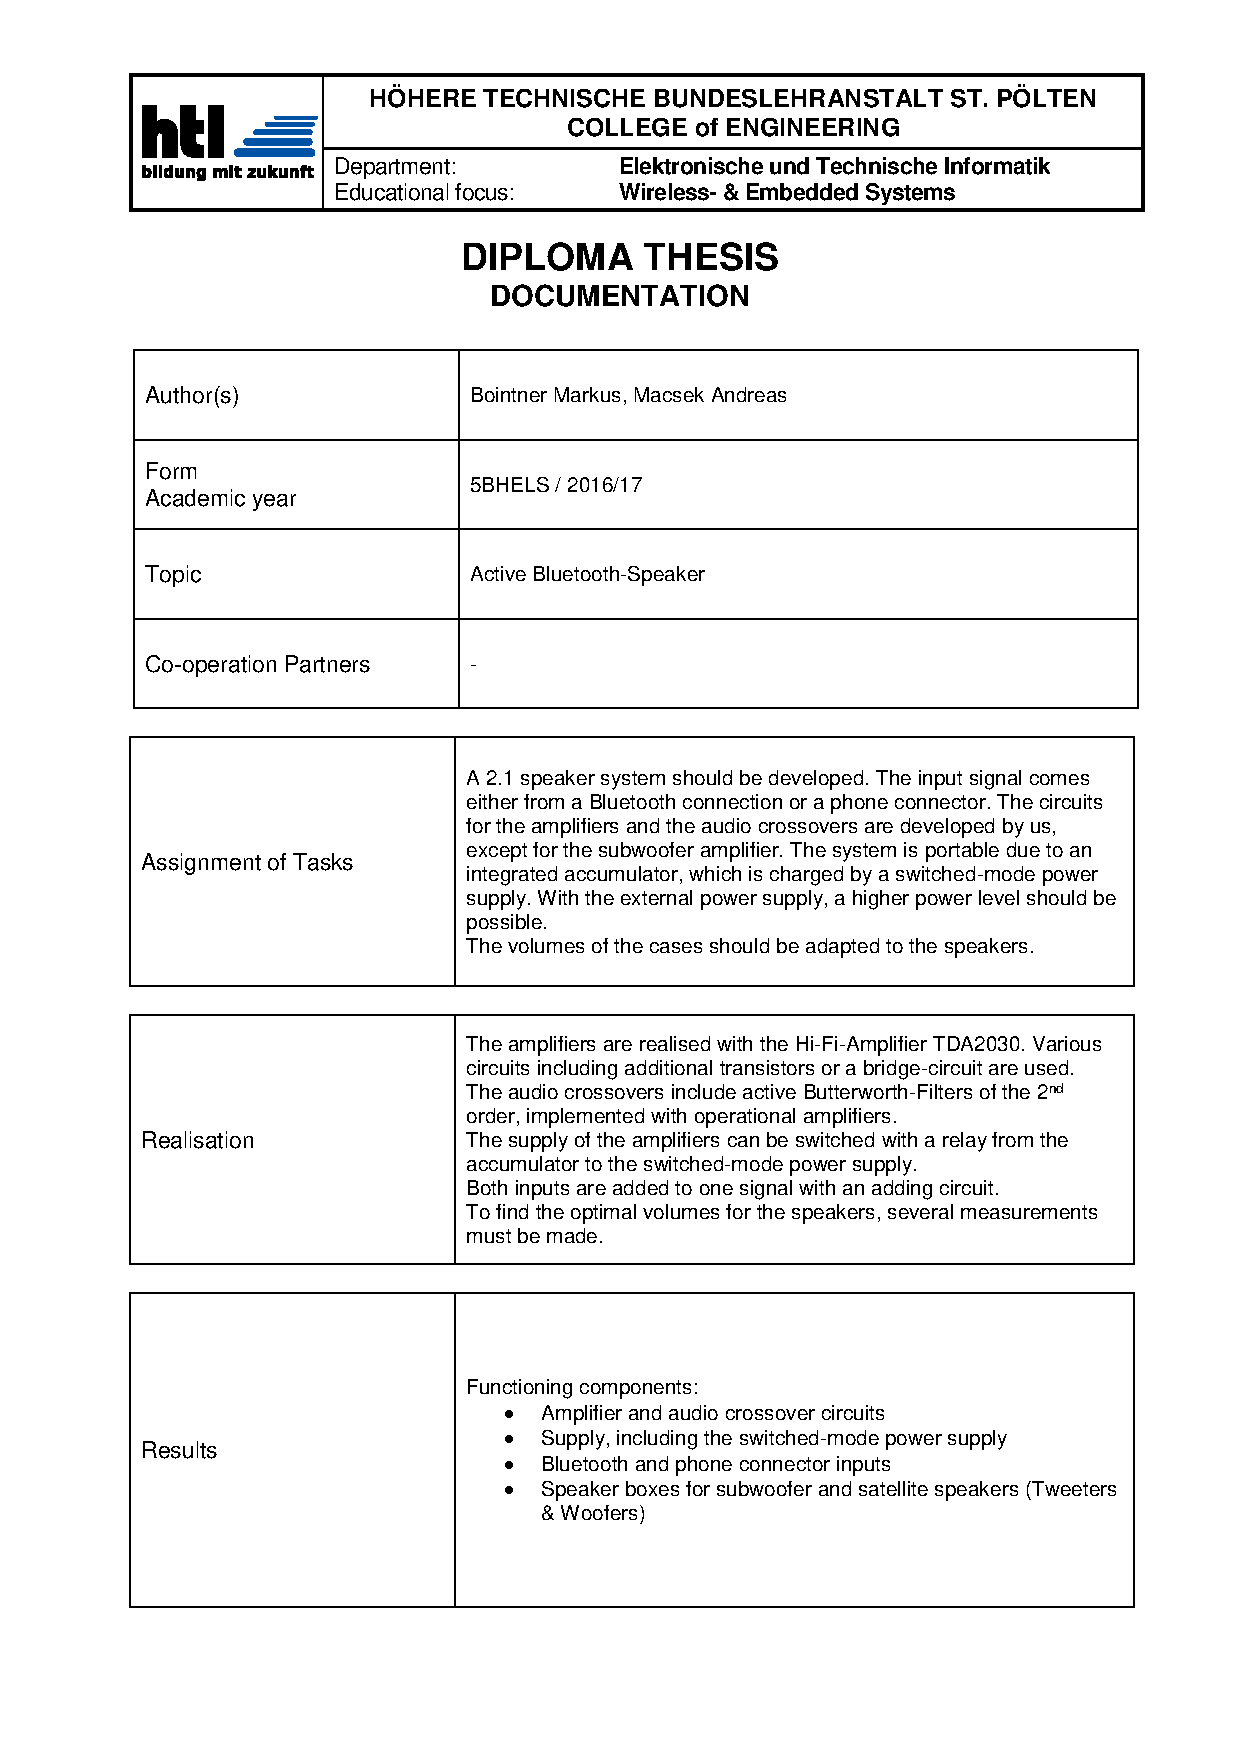
\includepdf[pages=-]{form/dokumentation-en.pdf}
%%======================================================%%

%% inhaltsverzeichnis ==================================%%
\tableofcontents
%%======================================================%%

%% HAUPTTEIL ===========================================%%
\responsible{Markus Bointner, Andreas Macsek}
\mainmatter

% Allgemeines über die Diplomarbeit
\chapter{Einleitung}
In diesem Kapitel wird erläutert, wie die Idee für diese Diplomarbeit entstanden ist und warum sie auch so verwirklicht wurde.

\section{Erste Idee} \label{sec:1.1}
Das Grundkonzept stammt von uns, also Markus Bointner und Andreas Macsek. Da wir beide von Musik begeistert sind, war es eine sehr interessante Idee für uns, selbst ein Lautsprechersystem zu entwickeln. Gleich zu Beginn war klar, dass wir noch ein kleines Extra mit einbauen wollten: eine Bluetooth-Ansteuerung.

\section{Weiterführende Gedanken} \label{sec:1.2}
Um all unsere Ideen zu verwirklichen, haben wir entschieden, diese Diplomarbeit ohne Firma und für den privaten Gebrauch zu entwickeln. Genauer gesagt ist das Lautsprechersystem dafür gedacht, im Freien oder in größeren Räumen Musik für kleinere Menschenmengen bereitzustellen. Das soll auch ohne externe Stromzufuhr funktionieren. Aus diesem Grund entstand dann die Idee einen Akku zu verbauen. Die manuelle Bedienung am Gerät soll mittels Ansteuerung eines Bluetooth-Moduls ermöglicht werden.


% Ziel der Diplomarbeit
\chapter{Individuelle Zielsetzung}

%\section{Ziele}\label{sec:2.1}
%Es soll ein 2.1-System entwickelt werden.
%Ein Mono-Subwoofer übernimmt den niedrigen Audiofrequenzbereich, während 2 weitere Lautsprecherboxen (auch genannt Satelliten-Boxen) - mit jeweils einem Hochton- und Tiefton-Lautsprecher - den Rest übernehmen.
%Dieser Aufbau wurde gewählt um einen Raum-Klang erzeugen zu können. \\
%Die Versorgung der Elektronik erfolgt entweder über Akku- oder Netzbetrieb.
%Jeder Hochton- und Tiefton-Lautsprecher bekommt einen eigenen Verstärker (so auch der Mono-Subwoofer). \\
%Das Audiosignal wird in verschiedene Frequenzbereiche aufgeteilt.\\
%
%%An Struktur neu anpassen
%Unsere Diplomarbeit kann grob in 2 Teile aufgeteilt werden:
%\begin{itemize}
%	\item Entwicklung der Elektronik
%	\item Auswahl und Messungen der Lautsprecher
%\end{itemize}
%Die Ziele der 2 Teile werden in diesem Kapitel kurz erläutert.


\section{Elektronik}\label{subsec:2.1.1}
Wie bereits in der Einleitung (\ref{sec:1.2}) erwähnt, ist das Projekt auch für den Akkubetrieb ausgelegt und benötigt daher eine passende Versorgungsschaltung.
Das Versorgungskonzept sieht einen 12V-Akku mit entsprechendem Ladegerät vor.
Dieses wurde zugekauft, da sich unser Projekt auf die Lautsprechermessung und -beschaltung konzentriert.
Bei Anschluss an eine Steckdose (nach CEE-Norm) übernimmt das vorgesehene Netzteil die Versorgung der Elektronik.
Wegen einer höheren Versorgungsspannung, als die 12V des vorgesehenen Akkus, steht bei Netzbetrieb eine höhere Leistung zur Verfügung. \\ \\
Es werden analoge Verstärker verwendet.
Gründe dafür sind:
\begin{itemize}
	\item Einfacher Aufbau
	\item Ausreichende Leistung und Effizienz für dieses Projekt
	\item Bewährte Technik für Audioverstärker
\end{itemize} 
Das Audio-Signal muss vor den Verstärkern noch gefiltert werden.
Diese Aufgabe übernimmt eine aktive Frequenzweiche.
Für den Mono-Subwoofer wird eine eigene Schaltung entwickelt, die nicht nur die unerwünschten Signalanteile herausfiltert, sondern zusätzlich das Stereo-Signal zu einem Mono-Signal addiert.\\ \\
%\newpage ??
Die Signalaufnahme erfolgt über Eingänge auf der Hauptplatine.
Auf dieser Platine befindet sich ein AUX-Eingang (3,5mm Klinkenbuchse).
Über ein passendes Klinkenkabel kann das Audiosignal von einem beliebigen Endgerät wiedergegeben werden.
Eine weitere Möglichkeit bietet das Bluetooth-Modul, welches sich ebenfalls, mittels Adapterplatine, auf der Hauptplatine befindet.
Durch dieses kann über Bluetooth-Funkverbindung mit einem beliebigen bluetoothfähigen Endgerät ebenso ein Audiosignal übertragen werden.
An der Hauptplatine werden des weiteren die Weichen und an diesen die Verstärker angeschlossen. 
Das schlussendlich verstärkte und gefilterte Audiosignal wird an den Lautsprechern abstrahlen.\\
Die Hauptplatine und die Adapterplatine für das Bluetooth-Modul wurden während einer Projektarbeit in der HTBLuVA St. Pölten entwickelt.
%Addierschaltung von Klinke und Bluetooth vielleicht erst später einbauen und erläutern

\section{Lautsprecher}\label{subsec:2.1.2}
Das Ziel für die Auswahl der Lautsprecher war es, möglichst laute Lautsprecher-Chassis mit möglichst gutem Frequenzgang (großer verwendbaren Frequenzbereich im Zusammenhang mit geringer Welligkeit [Kap. \ref{sec:8.6}]) zu finden.
Ein weiteres Ziel ist die Volumensverringerung der Box.
Dabei muss beachtet werden, dass sich die Klangqualität des in der Box verbauten Lautsprecher-Chassis mit variierendem Volumen, ebenfalls verändern kann.
Daher ist ein Boxenvolumen zu bestimmen, unter welchem die Klangqualität des Lautsprecher-Chassis nicht leidet.\\
Ein kleines Volumen ist nötig, da das fertige Lautsprecher-System auch für den Außenbereich verwendet werden soll, und daher leicht transportabel sein sollte.
Diesen Bedingungen fordern eine Optimierungsarbeit am Boxenvolumen.
%\begin{comment}
\section{Ziele}\label{sec:2.1}
Es soll ein 2.1-System entwickelt werden.
Ein Mono-Subwoofer übernimmt den niedrigen Audiofrequenzbereich, während 2 weitere Lautsprecherboxen (auch genannt Satelliten-Boxen) - mit jeweils einem Hochton- und Tiefton-Lautsprecher - den Rest übernehmen.
Dieser Aufbau wurde gewählt um einen Raum-Klang erzeugen zu können. \\
Die Versorgung der Elektronik erfolgt entweder über Akku- oder Netzbetrieb.
Jeder Hochton- und Tiefton-Lautsprecher bekommt einen eigenen Verstärker (so auch der Mono-Subwoofer). \\
Das Audiosignal wird in verschiedene Frequenzbereiche aufgeteilt.\\

%An Struktur neu anpassen
Unsere Diplomarbeit kann grob in 2 Teile aufgeteilt werden:
\begin{itemize}
	\item Entwicklung der Elektronik
	\item Auswahl und Messungen der Lautsprecher
\end{itemize}
Die Ziele der 2 Teile werden in diesem Kapitel kurz erläutert.
\end{comment}

\subsection{Elektronik}\label{subsec:2.1.1}
Wie bereits in der Einleitung (\ref{sec:1.2}) erwähnt, ist das Projekt auch für den Akkubetrieb ausgelegt und benötigt daher eine passende Versorgungsschaltung.
Das Versorgungskonzept sieht einen 12V-Akku mit entsprechendem Ladegerät vor.
Dieses wurde zugekauft, da unser Projekt sich auf die Lautsprechermessung und -beschaltung konzentriert.
Bei Anschluss an eine Steckdose (nach CEE-Norm) übernimmt das vorgesehene Netzteil die Versorgung der Elektronik.
Wegen einer höheren Versorgungsspannung als die 12V des vorgesehenen Akkus, steht bei Netzbetrieb eine höhere Leistung zur Verfügung. \\ \\
Es werden analoge Verstärker verwendet.
Gründe dafür sind:
\begin{itemize}
	\item Einfacher Aufbau
	\item Ausreichende Leistung und Effizienz für dieses Projekt
	\item Bewährte Technik für Audioverstärker
\end{itemize} 
Das Audio-Signal muss vor den Verstärkern noch gefiltert werden.
Diese Aufgabe übernimmt eine Aktive Frequenzweiche.
Für den Mono-Subwoofer wird eine eigene Schaltung entwickelt die nicht nur die unerwünschten Signal-Anteile herausfiltert, sondern auch noch das Stereo-Signal auf ein Mono-Signal addiert.\\ \\
%\newpage ??
Die Signalaufnahme erfolgt über Eingänge auf der Hauptplatine.
Auf dieser Platine befindet sich ein AUX-Eingang (3,5mm Klinkenbuchse).
Über ein passendes Kinkensteckerkabel kann das Signal von einem beliebigen Endgerät wiedergegeben werden.
Eine weitere Möglichkeit bietet das Bluetooth-Modul, welches sich ebenfalls, mittels Adapterplatine, auf der Hauptplatine befindet.
Durch dieses kann über Bluetooth-Funkverbindung mit einem beliebigen bluetoothfähigen Endgerät ebenso ein Audiosignal übertragen werden.
An der Hauptplatine werden des weiteren Filter und an diesen die Verstärker angeschlossen. 
Das schlussendlich verstärkte und gefilterte Audiosignal wird an einem Lautsprecher abstrahlen.\\
Die Hauptplatine und die Adapterplatine für das Bluetooth-Modul, wurden während einer Projektarbeit in der HTBLuVA St. Pölten entwickelt.
%Addierschaltung von Klinke und Bluetooth vielleicht erst später einbauen und erläutern

\subsection{Lautsprecher}\label{subsec:2.1.2}
Das Ziel für die Auswahl der Lautsprecher war es, möglichst laute Lautsprecher-Chassis mit möglichst gutem Frequenzgang (großer verwendbarer Frequenzbereich im Zusammenhang mit geringer Welligkeit [Siehe Kapitel \ref{sec:3.7}]) zu finden.
Ein weiteres Ziel ist die Verringerung des Volumens der Box.
Dabei muss beachtet werden, dass sich die Klangqualität des in der Box verbauten Lautsprecher-Chassis mit ändernden Volumen, ebenfalls verändern kann.
Daher ist ein Boxenvolumen zu bestimmen unter diesem die Klangqualität des Lautsprecher-Chassis nicht leidet.\\
Ein kleines Volumen ist nötig, da das fertige Lautsprecher-System auch für den Außenbereich verwendet werden soll und daher leicht transportabel sein sollte.
Aus diesen Bedingungen folgt eine Optimierungsarbeit am Boxenvolumen.       
    
% Erklärung verwendeter Software, ...
\chapter{Grundlagen und Methoden}
\responsible{Markus Bointner, Andreas Macsek}
\section{Blockschaltbild des Projekts}\label{sec:3.1}
Nach einigen Überlegungen über die beste Herangehensweise an dieses Projekt, wurde folgendes Blockschaltbild entwickelt:
\begin{figure} [H]
	\centering
	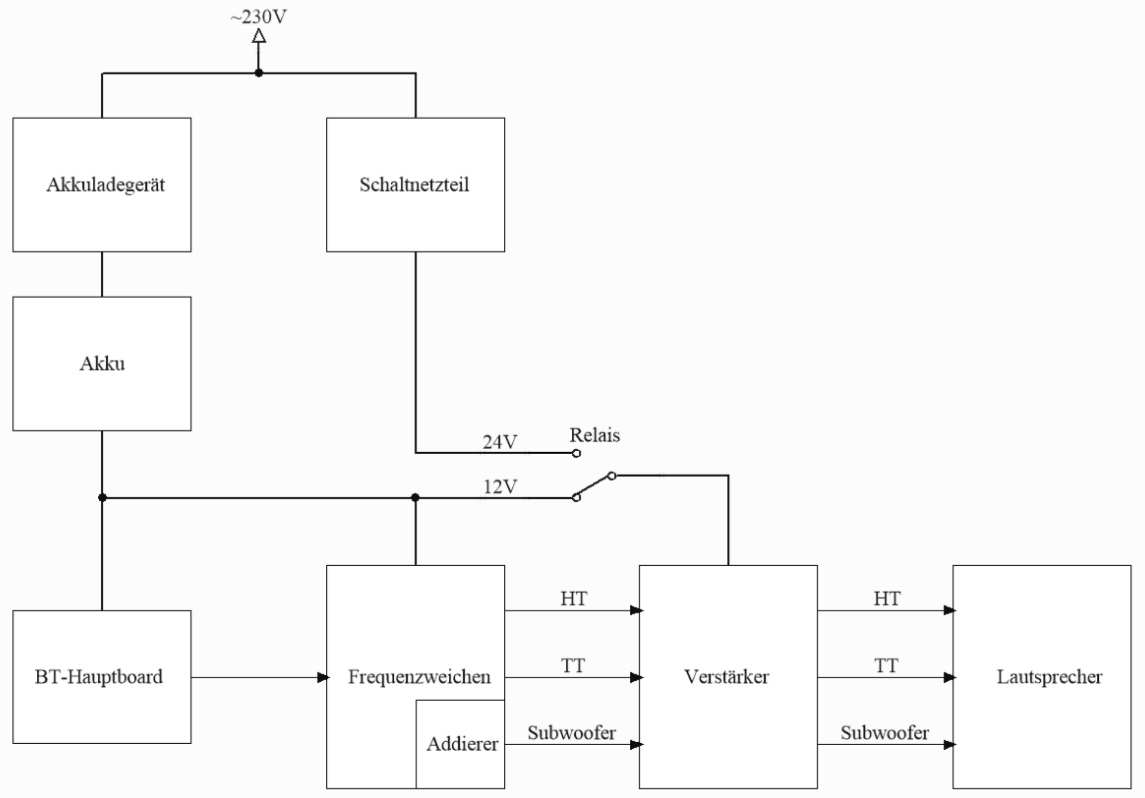
\includegraphics[width=1\textwidth]{img/blockschaltbild.png}
	\caption{Blockschaltbild}
	\label{fig:3.1.1}
\end{figure}
Ein wichtiger Teil des Projekts ist die Bluetooth-Hauptplatine (in Abb. \ref{fig:3.1.1} links unten).
Diese Platine verfügt über die Audio-Eingänge des Projekts.
Das Stereo-Audio-Signal kann mithilfe der BT-Hauptplatine mittels Klinkenbuchse oder Übertragung über Bluetooth (siehe: Kap. \ref{sec:3.3}) in die gesamte Schaltung eingespeist werden.
\\ \\
Dieses Stereo-Audio-Signal wird dann mithilfe der Frequenzweichen in 3 verschiedene Frequenzbereiche (Hochton-, Mittel-Tiefton- und Bassbereich) aufgetrennt.
\\
Tiefe Frequenzen (<150Hz) werden \enquote{L + R} (Stereo) addiert und über eine Mono-Tiefpass-Weiche gefiltert.
\\
Insgesamt gibt es dann also 5 Signale, die weiterverarbeitet werden:
\\ 
\begin{itemize}
	\item Hochton-Links
	\item Hochton-Rechts
	\item Mittel-Tiefton-Links
	\item Mittel-Tiefton-Rechts
	\item Mono-Bassbereich
\end{itemize}

Die verschiedenen Audio-Signale werden dann mit je einem Leistungs-Verstärker verstärkt.
Die Ausgangsleistung der Leistungs-Verstärker variiert je nach Frequenzbereichen.
Dies ist bedingt durch die verwendete Verstärkerschaltung.\\
Diese Schaltungen sind für:
\begin{itemize}
	\item \textbf{Hochtonbereich:}\\ TDA2030-Leistungsverstärker-Grundschaltung
	\item \textbf{Mittel-Tieftonbereich:}\\ TDA2030-Leistungsverstärker mit Leistungstransistoren
	\item \textbf{Bassbereich:}\\ TDA2030-Leistungsverstärker mit Leistungstransistoren in H-Brücke
\end{itemize}
Aus diesen Schaltungen erschließen sich folgenden maximale Ausgangsleistungen, bei asymmetrischer Spannungsversorgung von 24V und 1\% Klirrfaktor:\\
\begin{itemize}
	\item Hochton-Leistungsverstärker (an 8 Ohm): < 6W
	\item Mittel-Tiefton-Leistungsverstärker (an 4 Ohm): < 11W
	\item Bassbereich-Leistungsverstärker (an 4 Ohm): < 44W
\end{itemize}

Versorgt wird die Elektronik mit unter Akkubetrieb mit 12 V oder 24 V unter Netzbetrieb, genauere Erklärung im Kapitel \ref{sec:3.4}.
Somit befindet man sich an der Untergrenze der Leistungs-Verstärker-Schaltungen, diese sind maximal bis \enquote{+/- 22V} oder \enquote{+ 44V asymmetrisch} ausgelegt.
%Da eine Blei-Vlies-Batterie für das Projekt vorgesehen war und diese zumeist 12V liefern, ist die Entscheidung von einer 12V Spannungsversorgung sehr nahe.
%Andere Alternativen wie zB. LiPo-Akkus könnten mehr Spannung und Strom liefern, diese sind jedoch um einiges vorsichtiger zu Behandeln (sehr hohe Energiedichte) und daher auch umständlicher (Lade-Überwachung, Brandgefahr).

\newpage
\section{Mehrweg-Lautsprechersysteme}\label{sec:3.2}
Ein Lautsprecher ist ein Bauelement, das ein elektrisches Signal in ein akustisches Signal (20 Hz bis 20 kHz) umwandelt.
Dabei wird eine Membran in Schwingung versetzt, die wiederum die umgebende Luft zum Schwingen bringt und einen hörbaren Ton erzeugt.
\\ \\
Nun wird aber nicht jede Frequenz gleich gut von ein und demselben Lautsprecher abgestrahlt.
Durch die physikalischen Gegebenheiten strahlen große Membranen tiefe Frequenzen besser ab als hohe Frequenzen.
Daher ist es sinnvoll, mehrere Lautsprecher für verschiedene Frequenzbereiche zu verwenden.
Benannt werden diese verschiedenen Lautsprecher durch den Bereich in dem sie am besten funktionieren.
Beispielsweise Hochton-Lautsprecher oder Hochtöner für den Hochton-Bereich (>2,5 kHz).
Wie gut nun verschiedene Frequenzen von einem Lautsprecher abgestrahlt werden, ist in seinem Frequenzgang ersichtlich:
\begin{figure} [H]
	\centering
	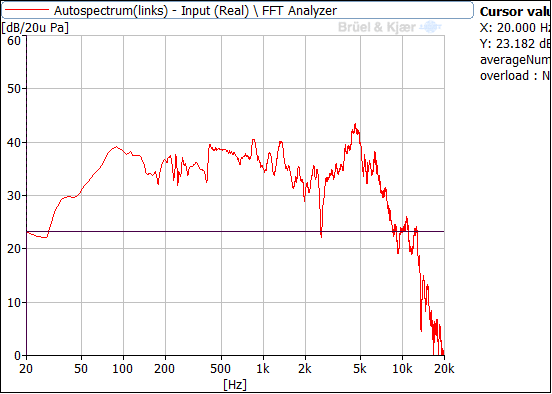
\includegraphics[width=1\textwidth]{img/LSMessung/TT1_9,17l_bestes.png}
	\caption{Beispiel eines Frequenzganges (Tieftöner PSS 297 58206)}
	\label{fig:3.2.1}
\end{figure}
Bei einem perfekten Lautsprecher würde diese Linie (Abb. \ref{fig:3.2.1}) eine parallele Gerade zur X-Achse bilden.
Da so ein Lautsprecher aber nicht existiert, werden verschiedene Frequenzen auch mit einem verschiedenen Schalldruckpegel vom Lautsprecher abgestrahlt.
\\
In dem Beispiel (Abb. \ref{fig:3.2.1}) wurde ein Tieftöner gemessen.
Das ist klar ersichtlich, da der Schalldruckpegel ab 5 kHz fast kontinuierlich fällt.
Tiefere Frequenzen werden, in einem gewissen Bereich, gleich wiedergegeben.
\\ \\
Je nach Frequenzbereich kann ein Ton vom menschlichen Ohr auch lokalisiert \mbox{werden}.
Hohe Frequenzen (<20 kHz) sind besser lokalisierbar als tiefe Frequenzen.
Bei sehr niedrigen Frequenzen (<150 Hz) ist der Ton gar nicht mehr lokalisierbar.
Diesen \mbox{Effekt} kann man nutzen und damit akustische Effekte erzeugen.
Einige Lautsprecher-Systeme, die diesen Effekt nutzen sind:
\begin{itemize}
	\item 2.0-System
	\item 2.1-System
	\item 5.1-System
\end{itemize}
Dabei steht die erste Zahl für die Anzahl der verteilten Lautsprecher und die zweite Zahl für die Anzahl der verwendeten Subwoofer.
\\
Je mehr verteilte Lautsprecher benutzt werden, desto bessere Raumklang-Effekte sind realisierbar.
Dadurch wird die Beschaltung aber auch komplizierter, da 5 verschiedene Audio-Signale verwendet werden.
\\ \\
Der Subwoofer ist ein spezieller Lautsprecher.
Er arbeitet im Bass-Bereich(20-150 Hz) und verarbeitet nur ein einziges Signal.
Diese Frequenzen sind nicht lokalisierbar, weshalb auch nur ein Subwoofer benötigt wird.
Meistens ist die Membran des Subwoofers um einiges größer als die Membran der anderen Lautsprecher.
Damit kann der Subwoofer mehr Luft in Bewegung setzen und somit einen höheren Schalldruckpegel erzeugen.
Um das zu ermöglichen benötigt der Subwoofer aber auch mehr Leistung als die anderen Lautsprecher.
\\ \\
In unserem Projekt haben wir uns direkt für ein 2.1-System entschieden, da sich dieses System am besten bewährt hat und für Musik ein Stereo-System völlig ausreicht.
Die zwei verteilten Boxen, auch Satelliten genannt, sind mit je einem Hochton- und einem Tiefton-Lautsprecher ausgestattet und werden über Kabeln mit der Hauptbox verbunden.
Damit sollen die Satelliten fast den gesamten Frequenzbereich für Audio (20 Hz bis 20 kHz) abdecken.
Der einzelne Subwoofer übernimmt den Bass-Bereich (<150 Hz) und sitzt in der Hauptbox.
Dort ist auch die gesamte Elektronik verbaut.

\section{Signalübertragung über Bluetooth}\label{sec:3.3}
Bluetooth ist eine moderne Funkschnittstelle für verschiedenste Anwendungen.
Unter anderem gibt es auch speziell für Audio-Anwendungen konzipierte Protokolle.
Die Übertragung läuft folgendermaßen ab:
\\
Zuerst muss das sendende Gerät (z.B. ein Smartphone) mit dem empfangenden Gerät (z.B. Bluetooth-Modul) verbunden werden.
Danach werden die gewünschten Daten ausgewählt.
In diesem Fall wären die Daten ein Musikstück.
Über Funk werden die digitalen Daten an das empfangende Gerät gesendet.
Nun muss das Bluetooth-Modul diese digitalen Daten wieder in ein analoges Signal umwandeln, welches dann weiterverarbeitet werden kann.
\\ \\
Dabei ist eine hohe Kompatibilität mit viele Geräten wichtig, weil es sehr viele verschiedene Versionen von Bluetooth gibt.
Da Bluetooth-Geräte meist abwärtskompatibel sind, ist es sinnvoll das Modul mit einer älteren BT-Version laufen zu lassen.
\\ \\
Nach ausführlicher Recherche wurde das Modul \enquote{XS3868} ausgewählt.
Der darauf verbaute Chip \enquote{OVC3860} von \enquote{OmniVision Technologies} hat sich bereits in vielen anderen Projekten bewährt, da er günstig ist und Funktionen wie \enquote{Play/Pause} bereitstellt.
\newpage
Im \enquote{OVC3860} (Abb. \ref {fig:3.3.1}) ist außer der Bluetooth-Verbindung auch noch ein Stereo-Audio-Prozessor verbaut.
Zusätzlich gibt es noch eine UART-Schnittstelle mithilfe man einige Einstellungen am Chip vornehmen kann.
Eine LiPo-Akku-Ladeschaltung ist ebenfalls vorhanden, wird aber in diesem Projekt nicht verwendet.
\\
Das Modul benötigt eine Versorgungsspannung von 3,3 V bis 4,2 V, wobei der Chip mit 1,8 V versorgt wird.
Diese Spannung (1,8 V) wird auf dem Modul erzeugt.
\\
Die verwendete BT-Version ist 2.0.
Einige GPIO-Pins sind auf das Modul herausgeführt um Funktionen wie \enquote{Play/Pause} zu ermöglichen.
Der Chip benötigt einen externen Speicher und eine Antenne (auf dem Modul) um ordnungsgemäß zu funktionieren.
\begin{figure} [H]
	\centering
	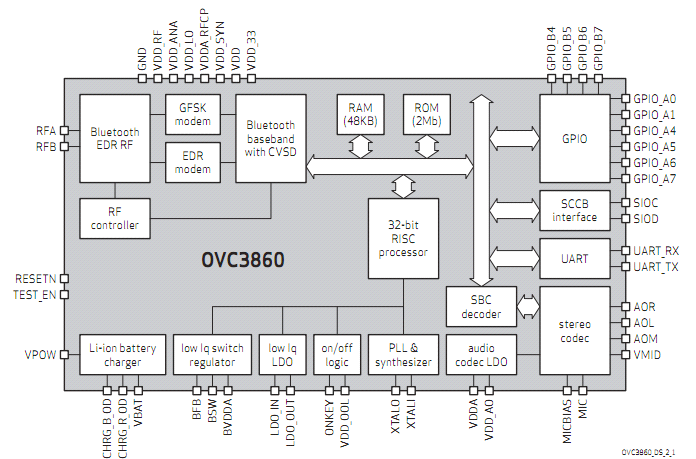
\includegraphics[width=1\textwidth]{img/BTModul/blockschaltbild.png}
	\caption[Blockschaltbild OVC3860]{Blockschaltbild OVC3860\footnotemark}\label {fig:3.3.1}
\end{figure}
\footnotetext{http://cxem.net/review/files/review24\_OVC3860.pdf,\\Zugriff: 11.03.2017}

\newpage
\section{Spannungsversorgung}\label{sec:3.4}
Die gesamte Box soll portabel sein, d.h. ohne externe Stromzufuhr funktionieren.
Dafür ist ein Akku notwendig.
Nach einigen Überlegungen haben wir uns für einen Blei-Vlies-Akku entschieden.
Gründe dafür sind:
\begin{itemize}
	\item Geringe Kosten
	\item Einfache Beschaltung
	\item Geringere Gefahr gegenüber Lithium-Akkus
	\item Wegen Vlies-Technik: Kein Auslaufen von chemischen Substanzen
\end{itemize}
Dieser Akku versorgt grundsätzlich die Elektronik mit 12 V und wird über ein passendes Ladegerät aufgeladen.
Da aber mit dieser, relativ geringen, Spannung nur eher kleine Leistungen zu erwarten sind, kam die Idee auf, die Verstärker bei externer Versorgung durch das Stromnetz (230 V / AC) mit einer größeren Spannung (24 V) zu versorgen.
Um das zu realisieren wird ein Netzteil, in unserem Fall ein Schaltnetzteil benötigt.
Falls das Gerät am externen Stromnetz hängt, wird die Versorgung der Verstärker automatisch mithilfe eines passenden Relais umgeschaltet.
Diese Lösung wurde gewählt, da sie sehr simpel ist und gut funktioniert.
Veranschaulicht wird das Konzept durch diese Schaltung:
\begin{figure} [H]
	\centering	
	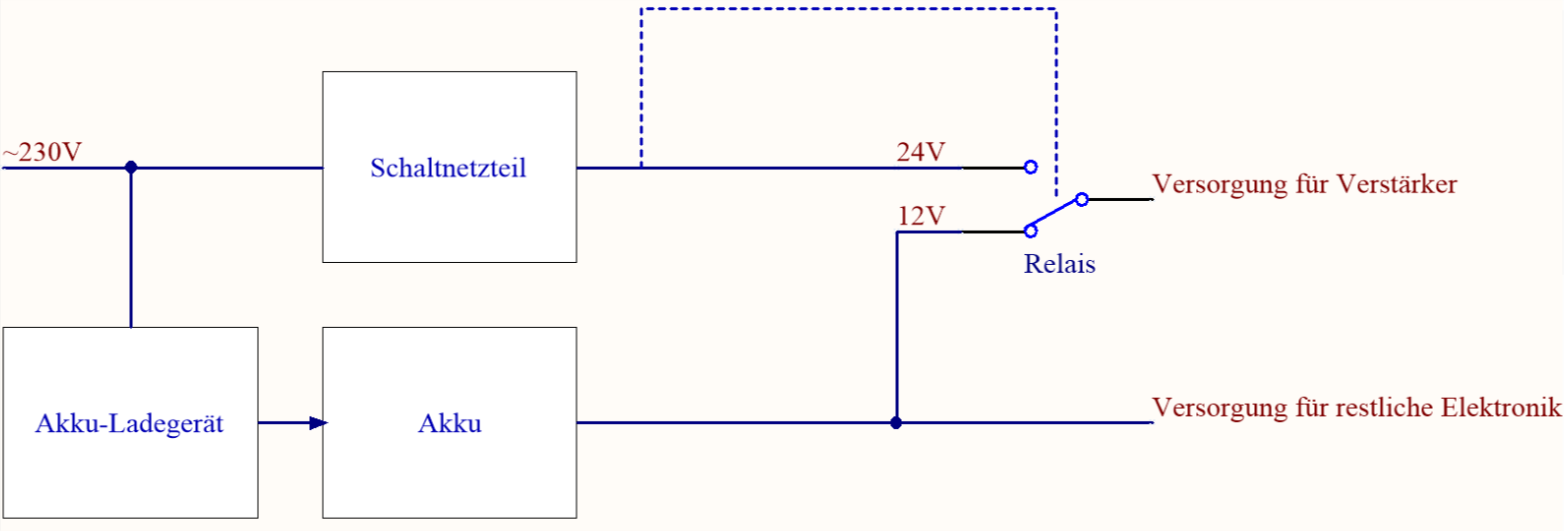
\includegraphics[width=1\textwidth]{img/Grundlagen/Versorgung.png}
	\caption{Versorgungskonzept}
	\label {fig:3.4.1}
\end{figure}
Das Lautsprecher-System kann somit bei Netzbetrieb die Musik lauter abspielen, als bei Akku-Betrieb.

% ANDERE VERSION
%Da das Projekt portabel sein soll, ist auch ein Akku (Vlies-Blei-Akku) eingebaut.
%Er versorgt die gesamte Elektronik mit 12 V bei Akkubetrieb.
%Aufgeladen wird er durch ein passendes Ladegerät, welches aber nicht von uns entwickelt wird.
%\\ \\
%Falls eine externe Stromversorgung über eine Steckdose (230V AC) gegeben ist, ändert sich die Versorgung der Verstärker.
%Während nun der Akku aufgeladen wird, schaltet ein Relais die Versorgungsspannung der Verstärker von 12 V auf 24 V um.
%Diese Spannung (24 V) wird durch ein Schaltnetzteil erzeugt.
%\\ \\
%Durch eine höhere Spannung können die Verstärker auch die Signale auf höhere Spannungen verstärken.
%Somit ergibt sich eine höhere Leistung an den Verstärkern aber auch an den Lautsprechern.
%Eine Leistungssteigerung an einem Lautsprecher entspricht einer Steigerung des Schalldruckpegels was wiederum eine höhere Lautstärke bewirkt.
%An den Verstärkern bewirkt eine höhere Leistung auch eine größere Wärmeentwicklung.
%Der verbaute Kühlkörper muss diese Wärme bei Akkubetrieb als auch bei Netzbetrieb ableiten können.
%\\ \\
%Das Lautsprecher-System kann somit bei Netzbetrieb die Musik lauter abspielen, als bei Akku-Betrieb.


% Erklärung der Messungen
\chapter{Auswahl der Lautsprecher-Chassis}
%\newpage
\section{Messaufbau und Messung}


\section{Lautsprecher für Hochton-Bereich}


\section{Lautsprecher für Tiefton-Bereich}


\section{Optimierung der Lautsprecher-Boxen}

\subsection{Eignung von verschiedenen Materialien zur Volumsverminderung}

\subsection{Subwoofer-Box}

\subsection{Box für Satelliten-Boxen}

\responsible{Markus Bointner}
%TD -- Kapitel 4.1 -- alle Labels darauf aufbauend

%\section{Allgemeines}\label{sec:5.1}
%Um die Charakteristika eines Lautsprechers zu beurteilen ist es wichtig den genauen Frequenzgang eines Lautsprecherchassis zu wissen. Dieser sagt aus, wie sich ein Lautsprecher bei bestimmten Frequenzen verhält. Der von uns gemessene Frequenzbereich beginnt bei 20Hz und endet bei 20kHz. Dieser Bereich wurde gewählt, da auch das menschliche Gehör nur in diesen Frequenzen aktiv ist.
%\begin{figure} [H]
%	\centering
%	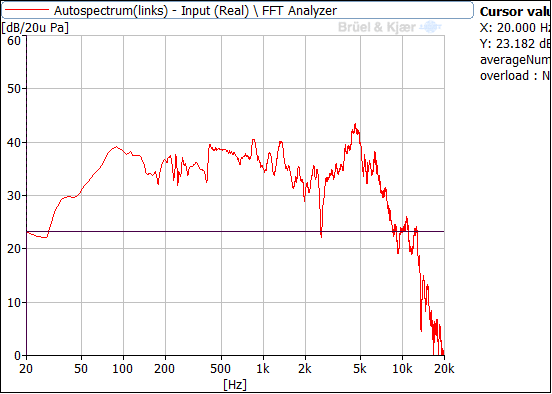
\includegraphics[width=1\textwidth]{img/LSMessung/TT1_9,17l_bestes.png}
%	\caption{Beispiel eines Frequenzganges (Tieftöner PSS 297 58206)}
%	\label{fig:5.1.1}
%\end{figure}
%Anhand dieses Beispiels kann man bereits sehr gut erkennen, wie sich der Schalldruckpegel (hier in dB angegeben) in Abhängigkeit der Frequenz verändert.\newpage
%Da der gemessene Lautsprecher in diesem Fall ein Tieftöner ist, sinkt der Pegel ab einer gewissen Frequenz sehr stark ab. Das bedeutet, dass diese Frequenzen wenig oder gar nicht von dem Lautsprecher abgestrahlt werden - also nicht hörbar sind.\\
%Die Qualität des Frequenzganges eines Lautsprechers hängt nun nicht direkt von dem absoluten Schalldruckpegel ab, sondern viel mehr von den relativen Schwankungen. Der absolute Pegel wird nämlich vom Signal des Verstärkers - im weiteren Sinne vom Benutzer - festgelegt. Das Wichtige dabei ist, was der Lautsprecher aus diesem Signal macht und so entsteht ein Frequenzgang.\\
%In diesem Fall werden hohe Frequenzen vom Lautsprecher \enquote{gedämpft} und somit nicht abgestrahlt.
%
%\subsection{Andere wichtige Eigenschaften eines Lautsprechers}\label{subsec:5.1.1}
%Ein Lautsprecher wird aber nicht nur durch seinen Frequenzgang definiert. Es gibt viele andere Eigenschaften, die auch unter dem Namen \enquote{Thiele-Small-Parameter}\footnote{https://de.wikipedia.org/wiki/Thiele-Small-Parameter,\\Zugriff: 11.02.2017} bekannt sind:
%% Quelle: https://de.wikipedia.org/wiki/Thiele-Small-Parameter
%\begin{itemize}
%	\item Äquivalentvolumen $ V_{as} $
%	\item Resonanzfrequenz $ F_{ms} $
%	\item Elektrische Güte $ Q_{es} $
%	\item Mechanische Güte $ Q_{ms} $
%	\item Gesamtgüte $ Q_{ts} $
%	\item Bewegte Masse $ M_{ms} $
%	\item Membranfläche $ S_{d} $
%	\item Nachgiebigkeit der Aufhängung $ C_{ms} $
%	\item Gleichstromwiderstand $ R_{e} $
%	\item Induktivität der Schwingspule $ L_{e} $
%	\item Verschiebevolumen $ V_{d} $
%	\item maximale Auslenkung $ X_{max} $
%	\item Kraftfaktor \emph{B × l}
%	\item mechanischer Verlustwiderstand $ R_{ms} $
%\end{itemize}
%Diese Eigenschaften, sowie auch die Impedanz \emph{Z}, beschreiben ebenfalls das Verhalten eines Lautsprechers. Sie wurden aber nicht von uns gemessen, weil der Fokus unseres Projekts eher an der Optimierung des Frequenzganges liegt. Die Thiele-Small-Paramter sind außerdem nicht veränderbar, also auch nicht optimierbar.

Um Lautsprecher mit geeigneten Eigenschaften auswählen zu können, müssen zunächst ausgewählte Lautsprecher gemessen und verglichen werden.

\section{Messaufbau und Messung}\label{sec:4.1}
Um überhaupt präzise Messungen an Lautsprechern durchführen zu können, benötigt man einen geeigneten Messraum.
Die HTBLuVA St. Pölten verfügt glücklicherweise über so einen reflexionsarmer Raum (Abb. \ref{fig:4.1.1}).
Dieser ist innen mit schalldämpfenden Material ausgekleidet und dämpft somit jede Schallwelle in ihm.
Die Anordnung und Struktur der an der Wand befestigten Absorberkeile ist ausschlaggeben dafür, dass der Raum eine relfexionsarme Umgebung aufweist.
Der Raum ist auf allen Seiten mit Absorberkeilen bestückt.
Es ist absichtlich ein 6-eckiger Raum um mögliche stehende Wellen noch besser zu unterdrücken.\\
Da es sich nicht um einen schalldichten Raum handelt ist es möglich, dass äußere Einflüsse (Trittschall, Erdbeben,...) das Messergebnis beeinflussen können.
Aus diesem Grund wurden die Messungen bei verdacht eines äußeren Einflusses erneut gemacht.

\newpage
\begin{figure} [H]
	\centering
	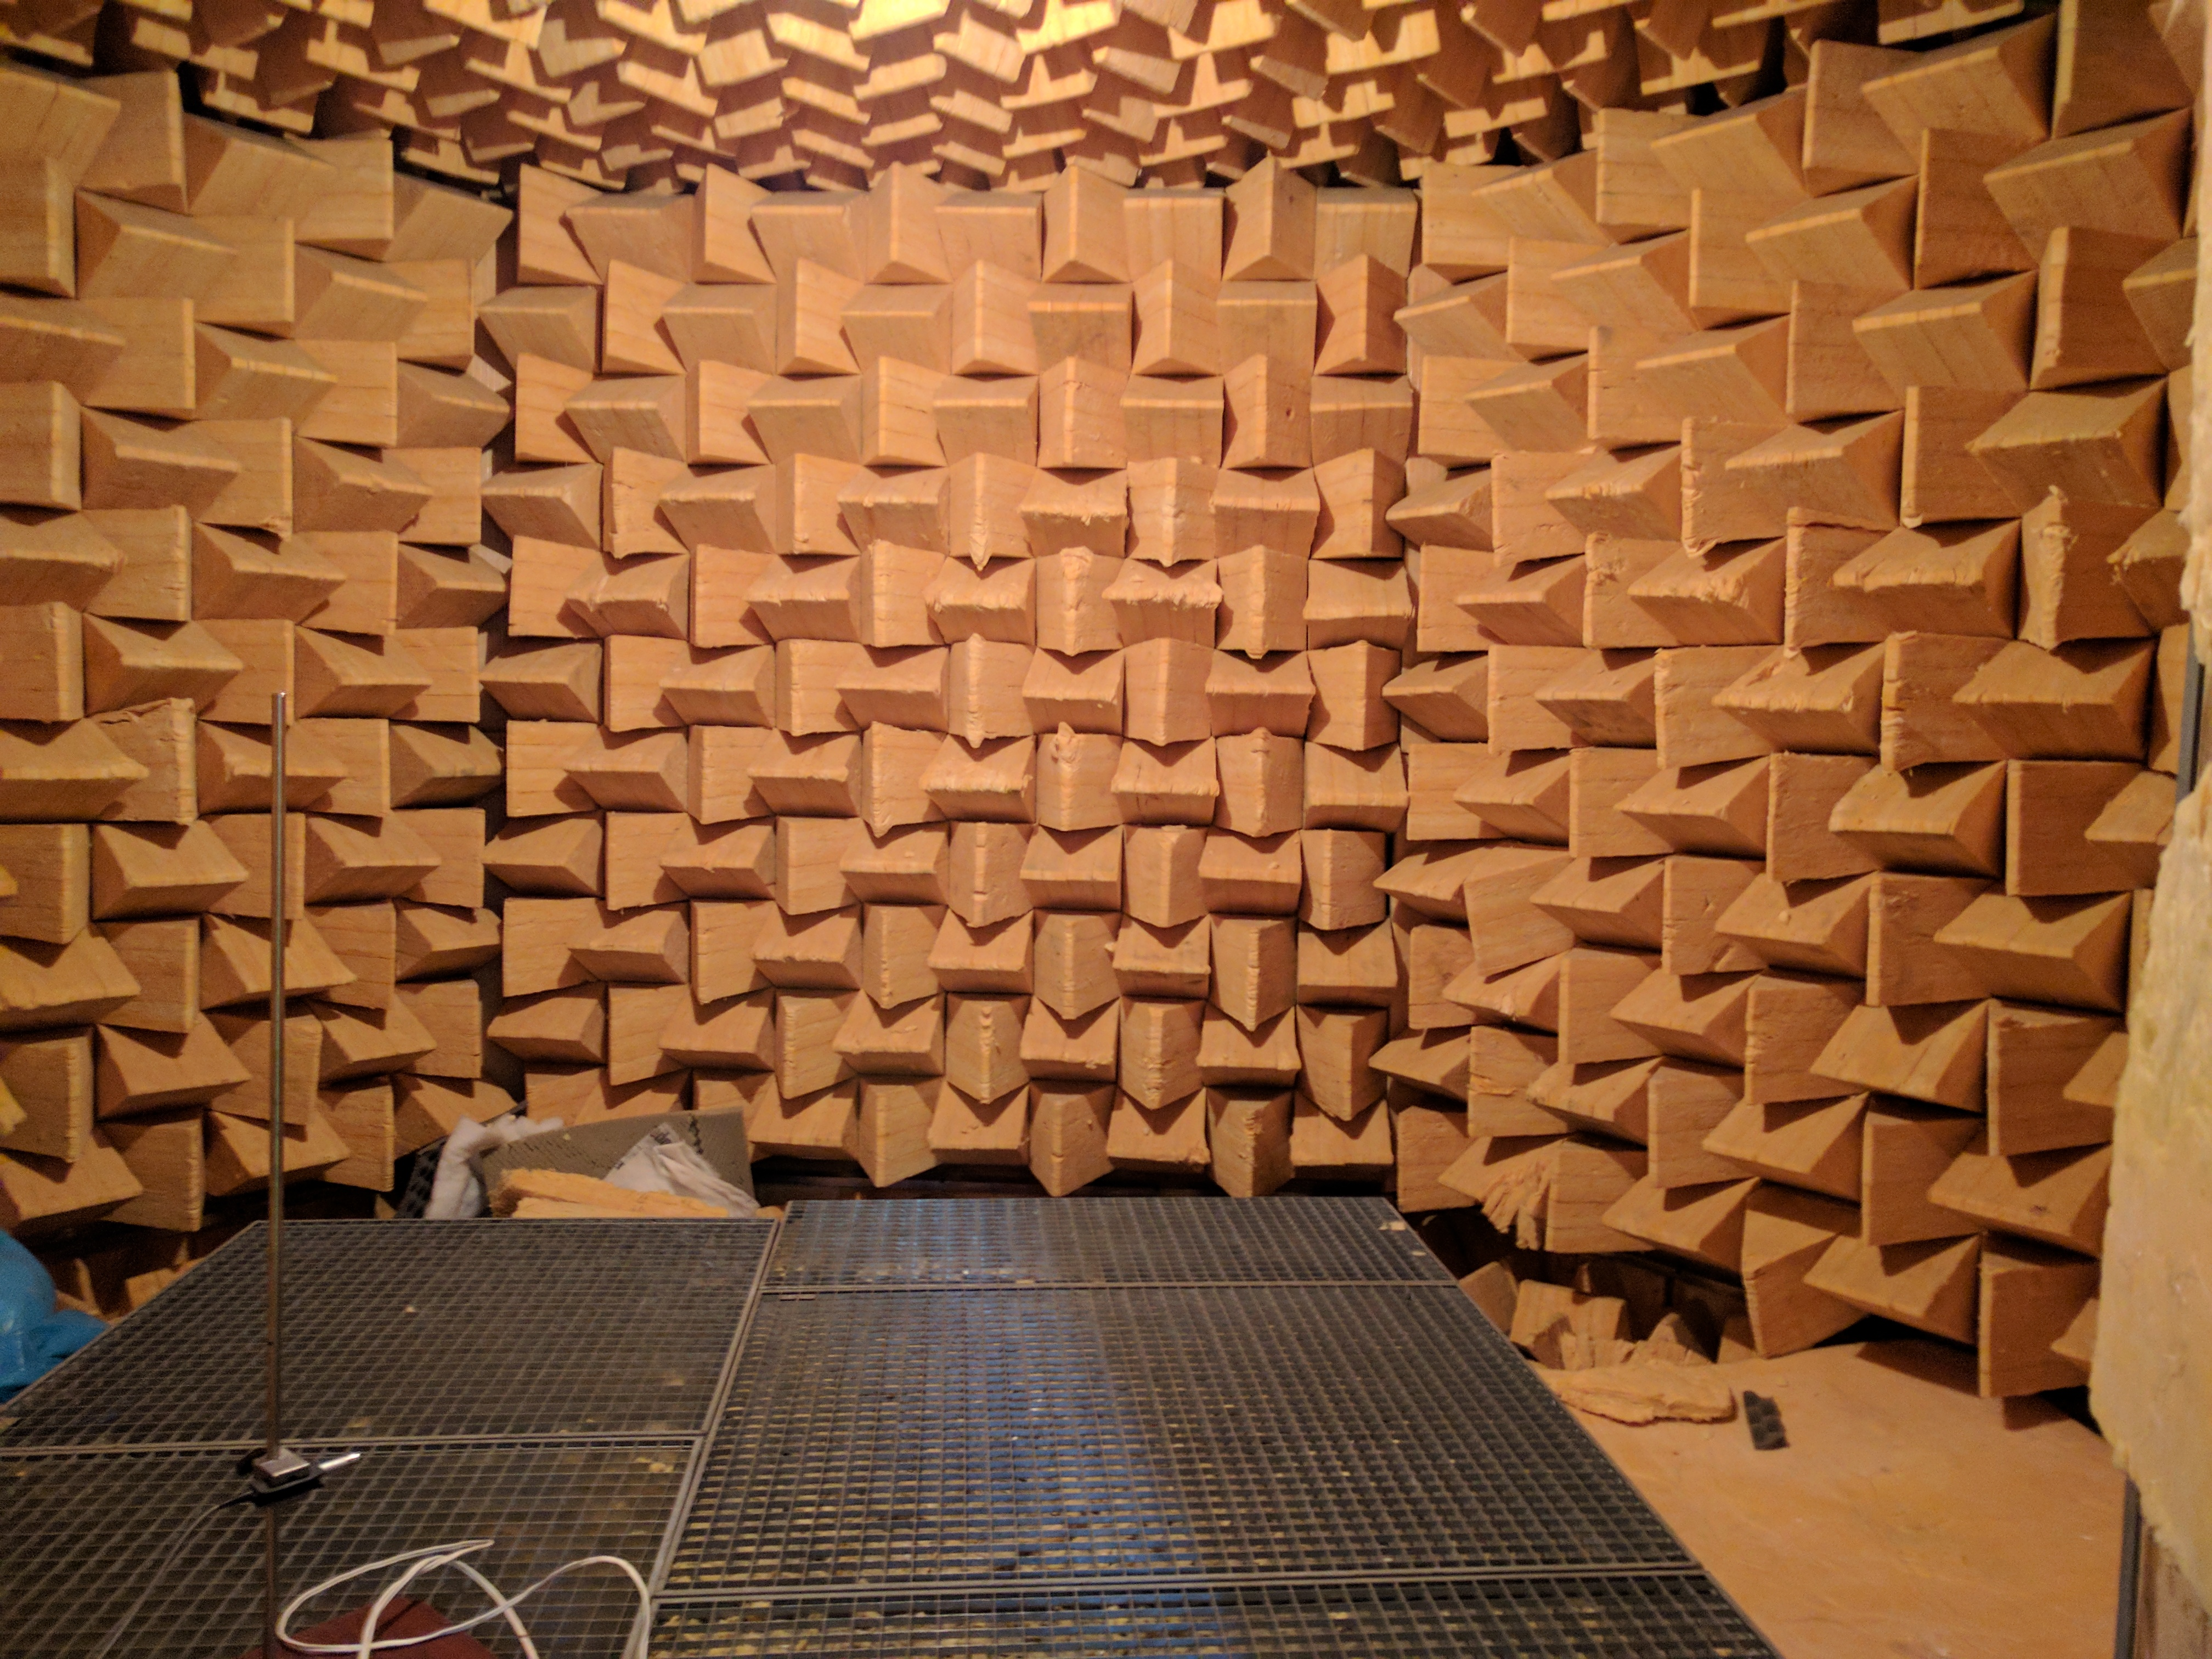
\includegraphics[width=1\textwidth]{img/LSMessung/akkustiklabor1.png}
	\caption{Reflexionsarmer Raum in der HTBLuVA St. Pölten}
	\label{fig:4.1.1}
\end{figure}
%\newpage
In diesem Raum (Abb. \ref{fig:4.1.1}) wurden alle Lautsprecher-Chassis gemessen.\\
Um auch ein passendes Mess-Signal erzeugen zu können ist noch weiteres Equipment nötig:
\begin{itemize}
	\item Mess-Software \enquote{PULSE LabShop Version 13.5.0} von \enquote{Brüel \& Kj\ae r}
	\item USB-Dongle zur Aktivierung der Software
	\item Kalibriertes Messmodul von \enquote{Brüel \& Kj\ae r}
	\item Kalibrierter Signal-Verstärker
	\item Kalibriertes Messmikrofon
	\item Optional: Oszilloskop
	\item Optional: Einstellbares Filter als Frequenzweiche
\end{itemize}

\newpage
\subsection*{Software}\label{subsec:4.1.1}
Als Software wurde \enquote{PULSE LabShop Version 13.5.0} von \enquote{Brüel \& Kj\ae r} verwendet.
Der Mess-PC basierte auf dem Betriebssystem \enquote{Windows XP}.
Um diese Software ordnungsgemäß verwenden zu können wird noch ein USB-Dongle benötigt.
Nur mit diesem Dongle lässt sich die Software, und somit die Messung, aktivieren.
\begin{figure} [H]
	\centering
	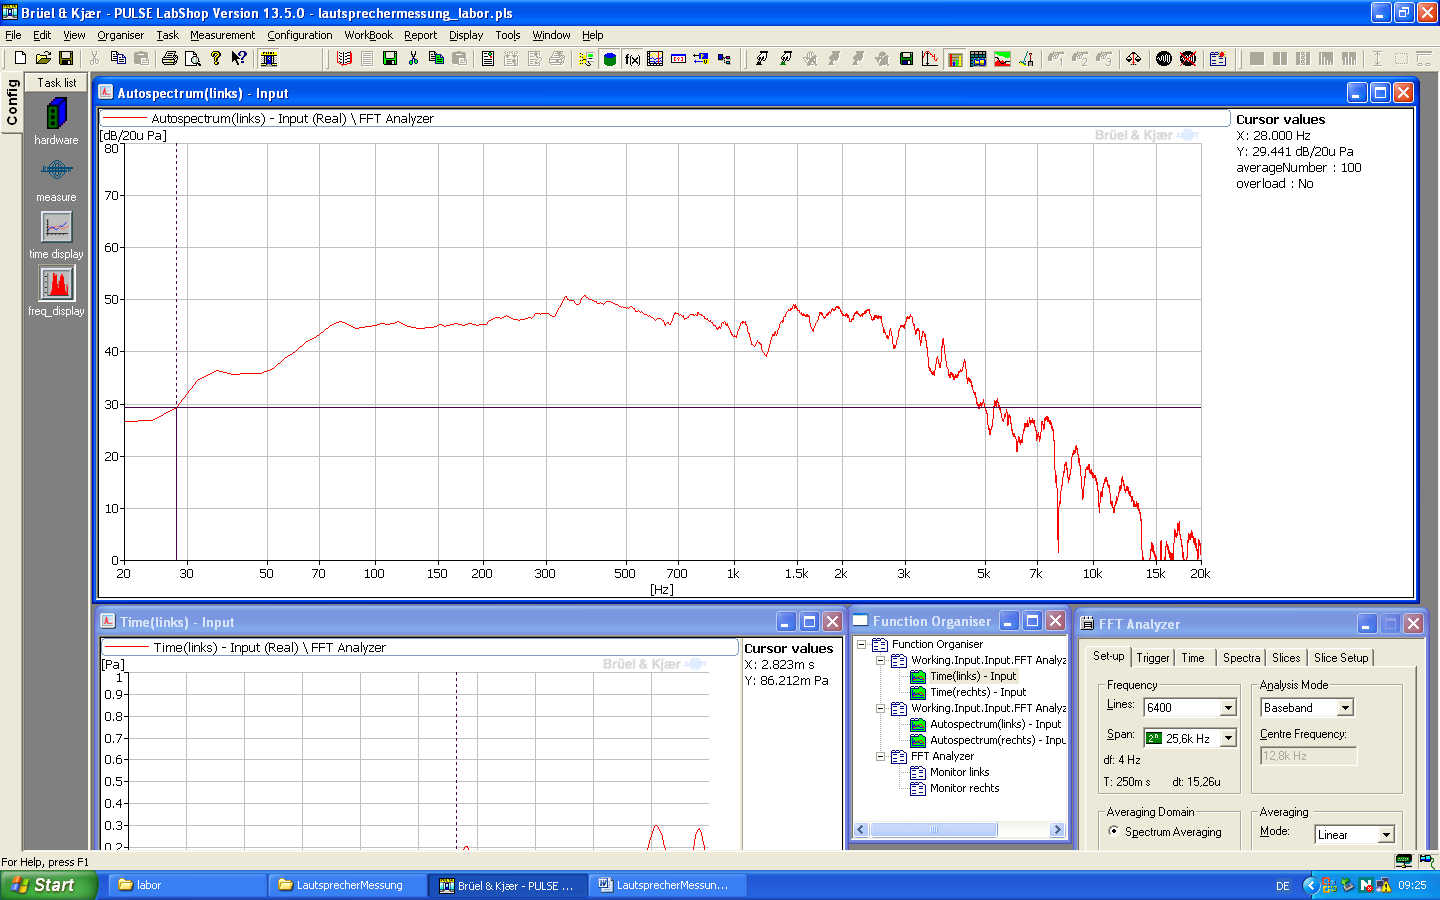
\includegraphics[width=0.8\textwidth]{img/LSMessung/VisatonMitSilikonMitWolle.png}
	\caption{Auschnitt aus der Software \enquote{PULSE LabShop}}
	\label{fig:4.1.1.1}
\end{figure}
In der Abbildung \ref{fig:4.1.1.1} ist bereits ein gemessener Frequenzgang eines Tieftöners zu sehen. Bei den Messungen wurde eine abgespeicherte vorkonfigurierte Datei verwendet, da man sonst immer wieder die nötigen Einstellungen treffen müsste.
Die Software ist damit auf alle verwendeten Komponenten abgestimmt und sendet auch das richtige Mess-Signal, ein (\enquote{Weißes Rauschen}), aus.
Mit einem Klick auf die Start-Taste beginnt der Messvorgang.
Es werden insgesamt 100 Messungen gemittelt um einen möglichst genauen Frequenzgang aufnehmen zu können.
Dies dauert in etwa 20s.
\\
Die Messeinstellungen sind je nach Wunsch veränderbar, ebenso wie die Angaben und Einheiten der 2 Achsen.
Die Frequenzachse ist logarithmisch von 20Hz bis 20kHz dargestellt.
Die Achse des Schalldruckpegels ist in der Einheit dB angegeben, da die Einheit für Schalldruck \enquote{Pascal} einen Bereich von µPa bis Pa darstellen müsste.
Das dB-Maß erleichtert die Veranschaulichung und macht die Kurve übersichtlicher.
In diesem Beispiel (Abb. \ref{fig:4.1.1.1}) ist der Bereich von 0dB bis 80dB gewählt.
Diese Einstellung wurde später geändert auf 0dB bis 60dB um möglichst vergleichbare Messungen zu erzeugen.\\
Eine logarithmischen Frequenzachse und eine Pegelachse von 0 bis 60 (in dB), wird normalerweise für den Vergleich von Lautsprecher-Chassis verwendet.

\newpage
\subsection*{Messmodul}\label{subsec:4.1.2}
Das Messmodul ist über ein Ethernet-Kabel mit dem PC und somit mit der Software verbunden.
Sobald der Befehl zum Start der Messung kommt, beginnt das Modul das Mess-Signal auszusenden und gleichzeitig über das angeschlossene Mikrofon die Ergebnisse aufzunehmen und daraufhin auszuwerten.
\\
Das Mess-Signal besteht aus einem \enquote{weißen Rauschen}.
Dieses Signal ist optimal für die Messung von Lautsprechern, da alle Frequenzen mit gleichem Pegel ausgesendet werden.
% Quelle: https://upload.wikimedia.org/wikipedia/commons/c/c1/White_noise.svg
% Quelle: https://upload.wikimedia.org/wikipedia/commons/3/3c/White_noise_spectrum.svg
\begin{figure} [H]
	\centering
	\subfloat{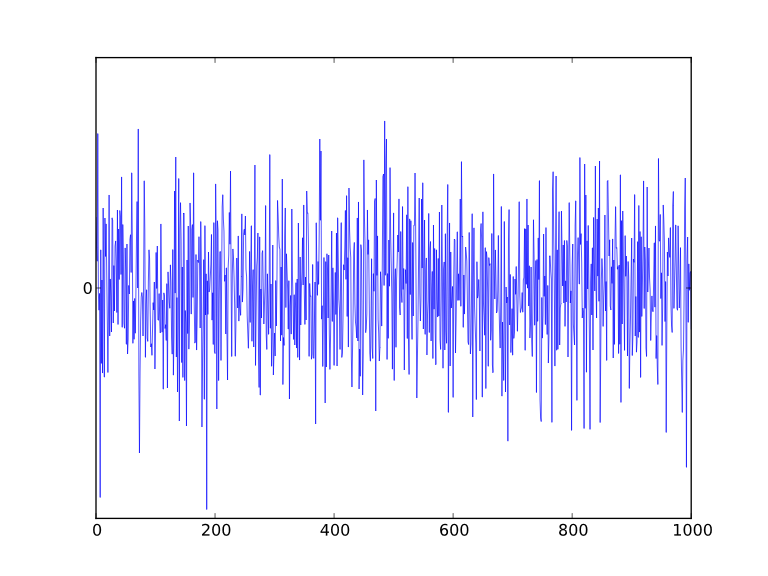
\includegraphics[valign=m,width=0.4\textwidth]{img/LSMessung/White_noise.png}}
	\subfloat{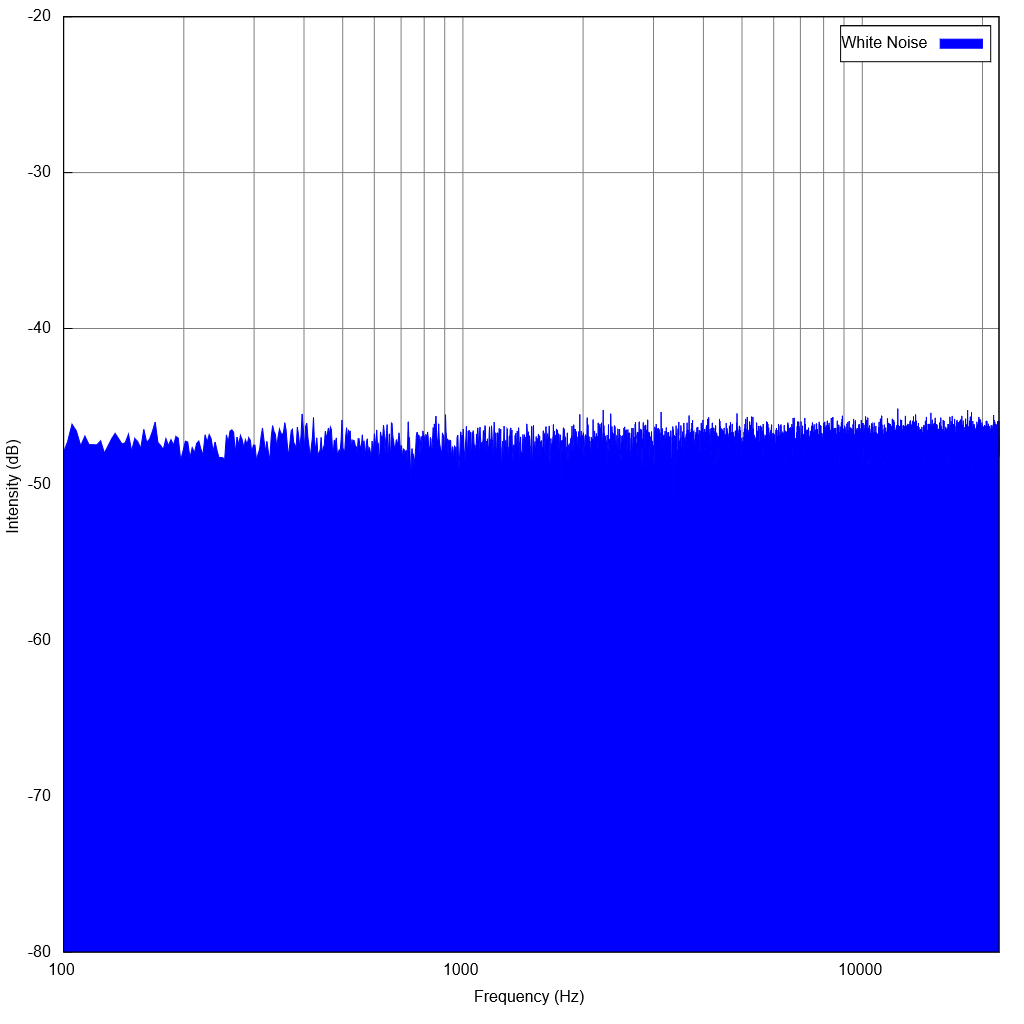
\includegraphics[valign=m,width=0.4\textwidth]{img/LSMessung/White_noise_spectrum.png}}
	\caption[Zeitfunktion und Spektrum von \enquote{weißem Rauschen}]{Zeitfunktion\footnotemark und Spektrum\footnotemark von \enquote{weißem Rauschen}}
	\label{fig:4.1.2.1}
\end{figure}
\footnotetext[2]{https://upload.wikimedia.org/wikipedia/commons/c/c1/White\_noise.svg,\\Zugriff: 11.02.2017}
\footnotetext[3]{https://upload.wikimedia.org/wikipedia/commons/3/3c/White\_noise\_spectrum.svg,\\Zugriff: 11.02.2017}
\begin{figure} [H]
	\centering
	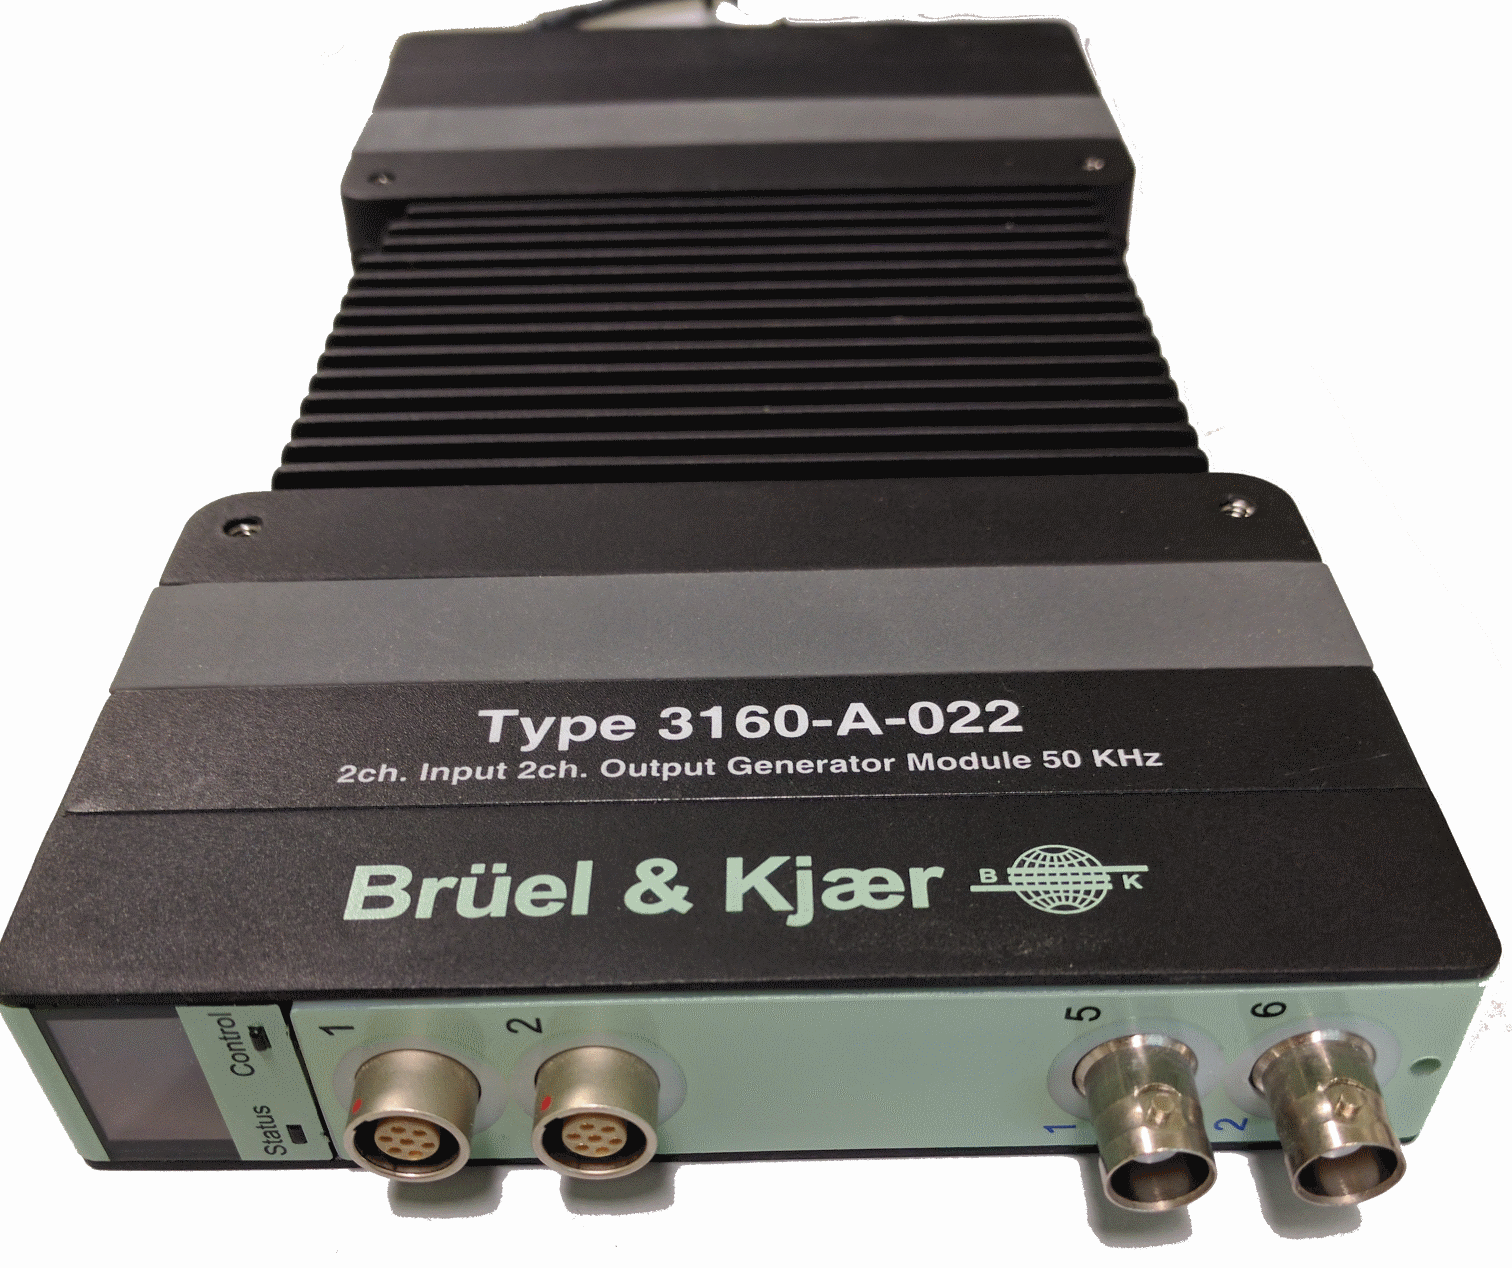
\includegraphics[width=0.4\textwidth]{img/LSMessung/modul_front.png}
	\caption{Messmodul}
	\label{fig:4.1.2.2}
\end{figure}

\newpage
\subsection*{Verstärker}\label{subsec:4.1.3}
Prinzipiell kann für diesen Aufbau jeder Leistungsverstärker verwendet werden.
In unserem Fall war ein kalibrierter \enquote{Brüel \& Kj\ae r Power Amplifier Type 2706} in Verwendung.
\\
Da meist nur ein Lautsprecher gemessen wird, benötigt man auch nur ein Signal (Mono, kein Stereo) zum Messen.
Der Verstärker verfügt über einen, in Stufen schaltbaren, Abschwächer und einen stufenlosen \enquote{Gain Control}.\\
Da die anderen Messkomponenten in dem Aufbau auch von der Firma  \enquote{Brüel \& Kj\ae r} sind, weist der Verstärker eine hohe Kompatibilität zum restlichen Equipment auf.
\begin{figure} [H]
	\centering
	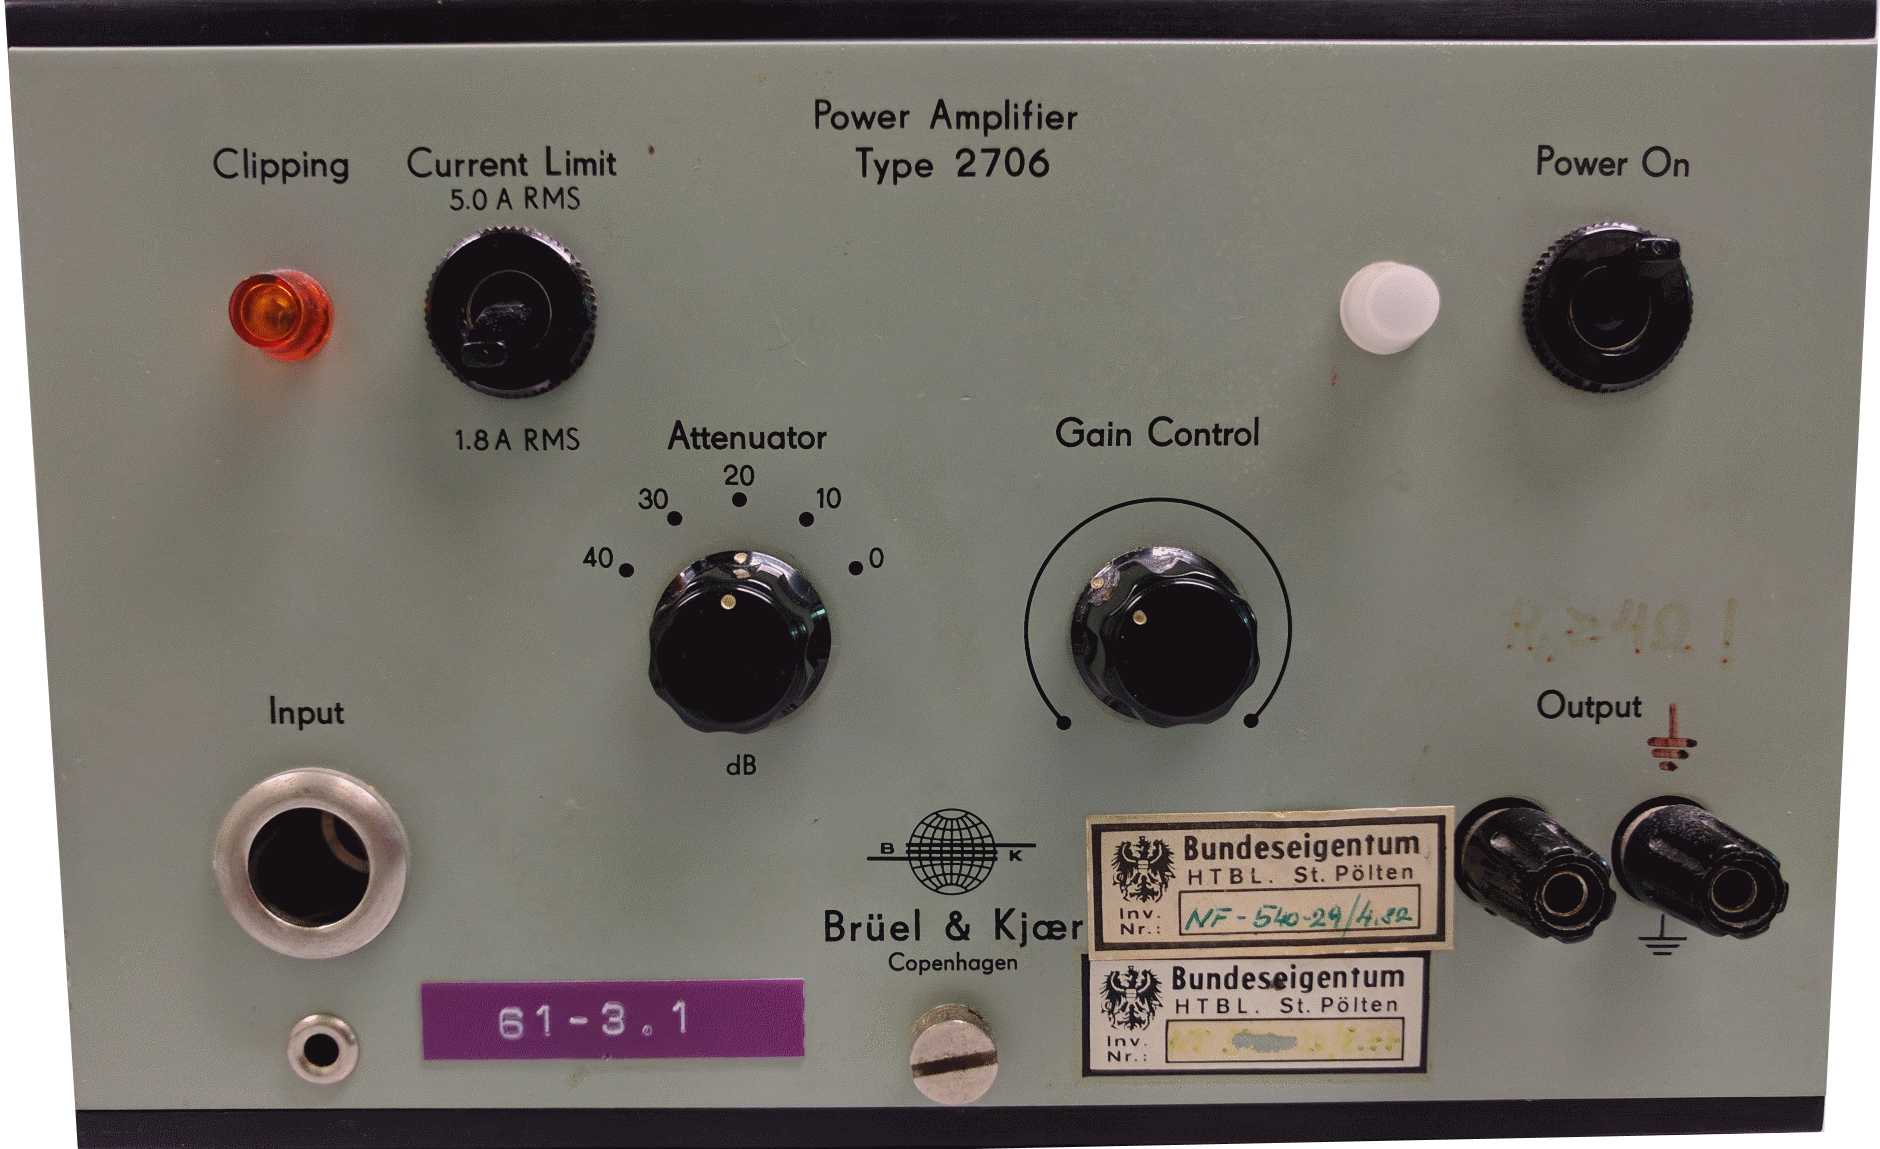
\includegraphics[width=0.4\textwidth]{img/LSMessung/verstaerker1V2.png}
	\caption{\enquote{Brüel \& Kj\ae r Power Amplifier Type 2706}}
	\label{fig:4.1.3.1}
\end{figure}

\subsection*{Messmikrofon}\label{subsec:4.1.4}
Um den Schalldruckpegel möglichst präzise messen zu können, wird auch ein dementsprechend genaues und kalibriertes Messmikrofon benötigt.
Das bei uns verwendete Messmikrofon war das \enquote{Brüel \& Kj\ae r Type 2669}.
\\
Ebenfalls wichtig ist die Ausrichtung des Messmikrofons.
Es sollte immer auf den Lautsprecher, in der Höhe und Seitlich, zentriert angebracht werden.
Die Entfernung zum Messobjekt (1 m) muss bei verschiedenen Lautsprechern gleich bleiben, um vergleichbare Messungen zu ermöglichen.
Bei einem Zwei-Weg-System (Hoch- und Tieftöner) wurde das Mikrofon (vertikal gesehen) zwischen den Lautsprechern befestigt.
\begin{figure} [H]
	\centering
	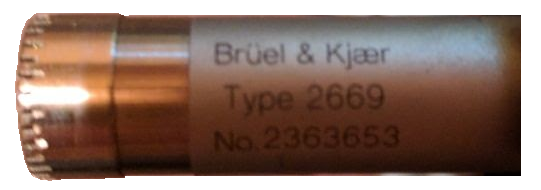
\includegraphics[width=0.4\textwidth]{img/LSMessung/mikroV2.png}
	\caption{Messmikrofon \enquote{Brüel \& Kj\ae r Type 2669}}
	\label{fig:4.1.4.1}
\end{figure}

%TD -- Kapitel 4.2 -- alle Labels darauf aufbauend

%\newpage
\section{Lautsprecher für Tiefton-Bereich} \label{sec:4.2}
\subsection*{Einleitung} \label{subsec:4.2.1}
Tiefton-Lautsprecher sind, wie der Name bereits andeutet, für den unteren Frequenzbereich gedacht und konzipiert.
In diesem Projekt werden Tiefton-Lautsprecher an zwei verschiedenen Positionen verwendet:
\begin{itemize}
	\item im Subwoofer und 
	\item in den Satellitenboxen
\end{itemize}
Es ist so angedacht, dass der Subwoofer (Mono) nur die sehr niedrigen Frequenzen übernimmt.
Er ist bis ca. 150 Hz aktiv.\\
In den Satellitenboxen ist jeweils ein kleinerer Tiefton-Lautsprecher verbaut, um den Übergang zwischen sehr tiefen und hohen Frequenzen zu bilden.
Diese zwei Lautsprecher (Stereo) arbeiten ebenfalls bei niedrigen als auch bei mittleren bis hohen Frequenzen.
Die Grenze des Satelliten-Tiefton-Lautsprechers liegt bei ca. 5 kHz.
Somit wird die Frequenzweiche für diese Frequenz berechnet und konzipiert.

\subsection*{Ziele} \label{subsec:4.2.2}
Der Lautsprecher für die Subwoofer-Box muss größer und leistungsfähiger sein, um die richtig tiefen Frequenzen möglichst gut abzustrahlen.
Da er nur bis ca. 150 Hz aktiv ist, sollte der Frequenzgang genau in diesem Bereich einen hohen Schalldruckpegel aufweisen.
Der Rest des Frequenzganges ist nicht so wichtig, da der Lautsprecher auch nicht in einem höheren Bereich verwendet wird. \\
Bei den Satelliten-Lautsprechern ist der ganz tiefe Frequenzbereich (< 150 Hz) nicht so ausschlaggebend.
Wichtiger ist dafür eine niedrige Welligkeit (siehe Kapitel \ref{sec:8.6}) bis 5 kHz, um den mittleren Frequenzbereich gut abstrahlen zu können.\\ \\
%Welligkeit könnte man vielleicht auch erklären als Grundlage -- @Bointii
Der Messvorgang und -aufbau wurde bereits im Kapitel \ref{sec:4.1} erläutert.
Nach diesem Prinzip wird bei allen Messungen vorgegangen.
%Nach diesem Prinzip wird bei fast allen Messungen vorgegangen.

\newpage
\subsection*{Subwoofer} \label{subsec:4.2.3}
Bereits zu Beginn der Diplomarbeit wurde ein großer Tiefton-Lautsprecher eingekauft.\\
Dieser wurde in verschiedenen Volumina gemessen.\\
Außerdem wurden Vergleichsmessungen mit einem zweiten Tiefton-Lautsprecher durchgeführt.
\begin{figure} [H]
	\centering
	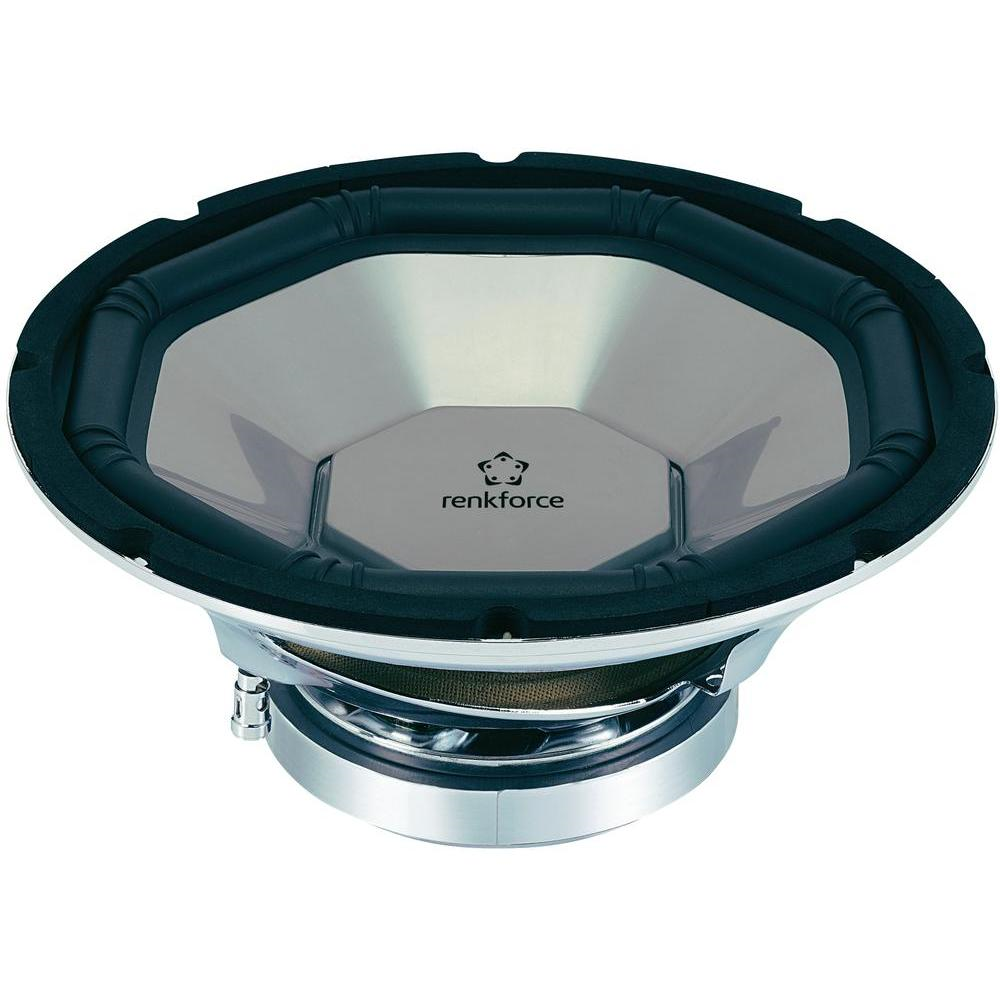
\includegraphics[width=0.5\textwidth]{img/LSMessung/TT/renkforce_B12123.png}
	\caption[\enquote{Renkforce B12123}]{\enquote{Renkforce B12123}\footnotemark}
	\label{fig:4.2.3.1}
\end{figure}
\footnotetext{https://www.conrad.at/de/auto-subwoofer-chassis-300-mm-500-w-renkforce-4-370335.html,\\Zugriff: 17.02.2017}
Dieser Lautsprecher wurde ausgewählt, weil er einen vergleichsweise hohen Schalldruckpegel bei tiefen Frequenzen aufweist und laut Angaben des Herstellers nur ein geringes Boxenvolumen benötigt.
Kurze Spezifikationen des Subwoofers sind:
\begin{itemize}
	\item Maximale Spitzenbelastbarkeit 500 W
	\item Maximale RMS-Belastbarkeit 200 W
	\item Durchmesser 30 cm
	\item Schalldruck 93 dB
	\item Impedanz 4 $\Omega$
\end{itemize}
Genauere Angaben findet man im Datenblatt des Lautsprechers (Kap. \ref{sec:8.7}).
Da man eine Box einfacher verkleinern kann als vergrößern, wurde eine Box mit einem Volumen von 149 l für die Messungen verwendet.
Die Box wurde aus Holz gefertigt und mit Silikon abgeschlossen, um mögliche Luftlöcher zu schließen.
Als Vergleichslautsprecher wurde ein \enquote{Visaton WPC30} gemessen.

\newpage
Diese Messungen wurden zu Beginn der Diplomarbeit durchgeführt und daher sind die Ergebnisse so aufgenommen, dass die Einstellungen der Software sichtbar sind. % Ideale Messung beschreiben?
Um die Aufnahmen ansehnlicher zu machen wurde der Frequenzgang durch Nachbearbeitung ausgeschnitten, sodass im Gegensatz zur Abbildung \ref{fig:4.1.1.1} in den nachfolgenden Bildern (ab Abb. \ref{fig:4.2.3.2}) nur die zum Vergleich relevanten Kurven dargestellt werden.\\
Die zwei Subwoofer-Chassis wurden einmal mit und einmal ohne Wolle in der Box gemessen.
\begin{figure} [H]
	\centering
	\subfloat{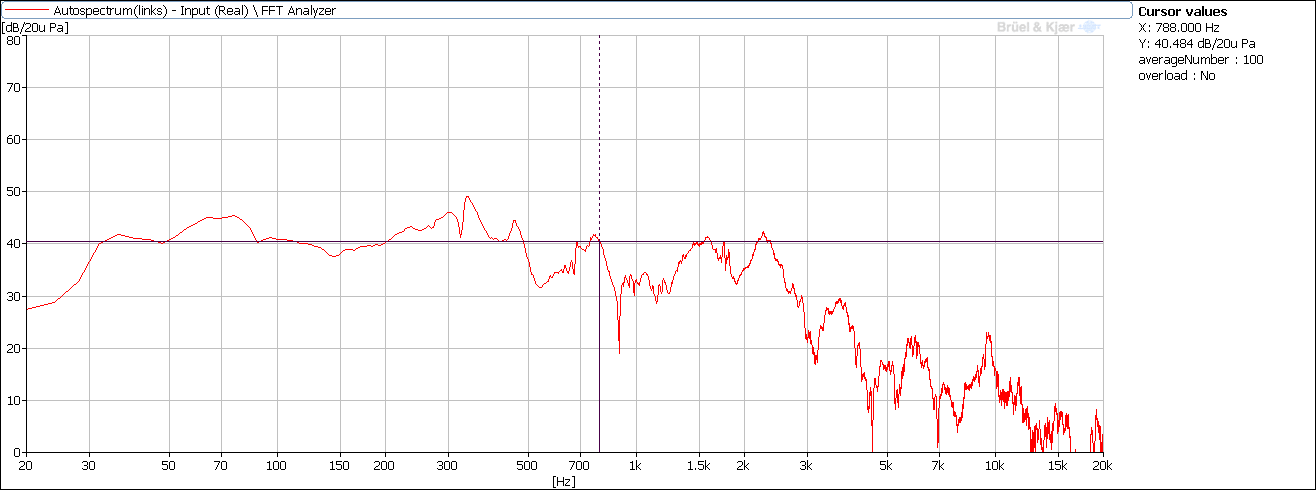
\includegraphics[width=1\textwidth]{img/LSMessung/TT/RenkforceOhneWolleMitSilikonV2.png}}\quad
	\subfloat{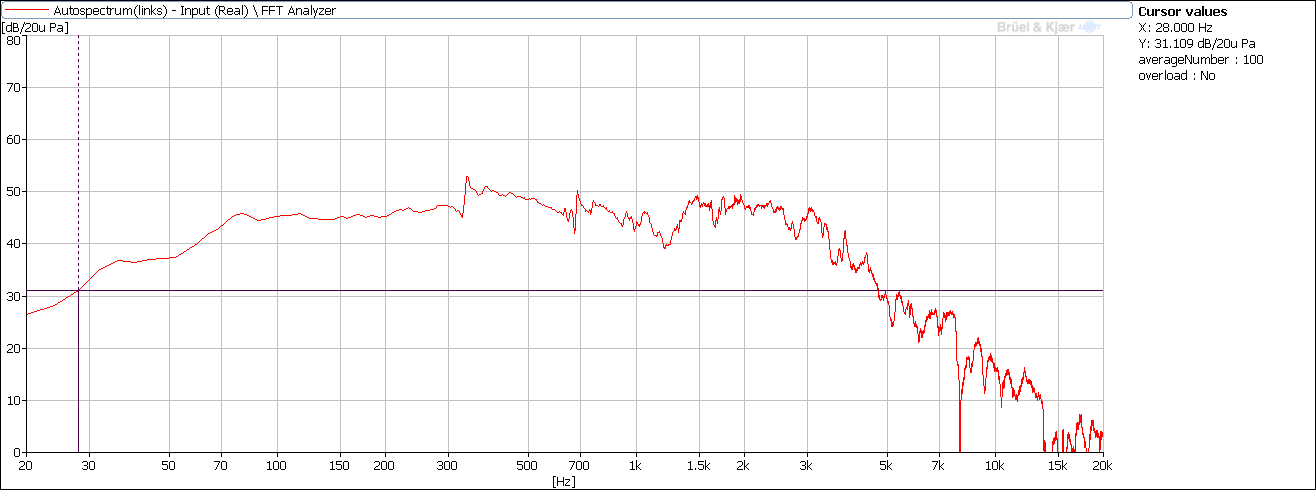
\includegraphics[width=1\textwidth]{img/LSMessung/TT/VisatonMitSilikonOhneWolleV2.png}}
	\caption{Subwoofer-Messung ohne Wolle\\ \enquote{Renkforce} (oben) und \enquote{Visaton} (unten) | Boxenvolumen: 149 l}
	\label{fig:4.2.3.2}
\end{figure}
Bei diesem Vergleich ist sichtbar, dass der Frequenzgang des \enquote{Visaton}-Tieftöners allgemein \enquote{gerader} ist und somit eine geringere Welligkeit aufweist.
Wenn man allerdings nur auf die tiefen Frequenzen (< 150 Hz) achtet, die auch verwendet werden, ist festzustellen, dass der Schalldruckpegel des \enquote{Renkforce} einen höheren Wert aufweist.
Da der Lautsprecher zusätzlich in diesem Bereich auch noch eine geringe Welligkeit aufweist, ist er zu bevorzugen.
\newpage
Eine weitere Messung mit Wolle in der Box wurde deshalb durchgeführt, weil beide Frequenzgänge bei ca. 300 Hz eine ähnliche Unregelmäßigkeit aufweisen.
Die Auswirkungen auf das Messergebnis sind folgende:
\begin{figure} [H]
	\centering
	\subfloat{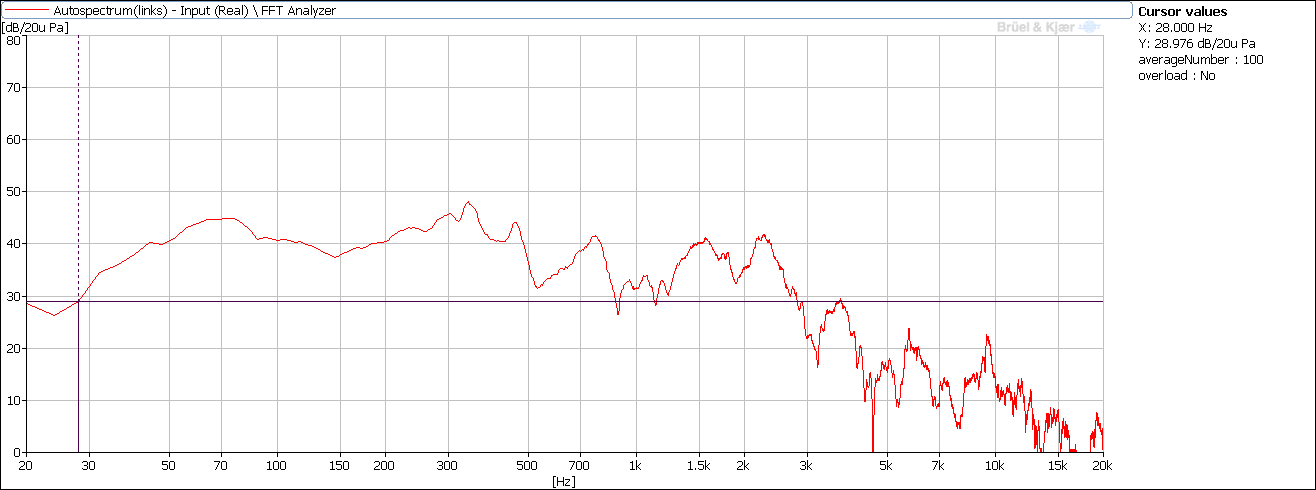
\includegraphics[width=1\textwidth]{img/LSMessung/TT/RenkforceMitWolleMitSilikonV2.png}}\quad
	\subfloat{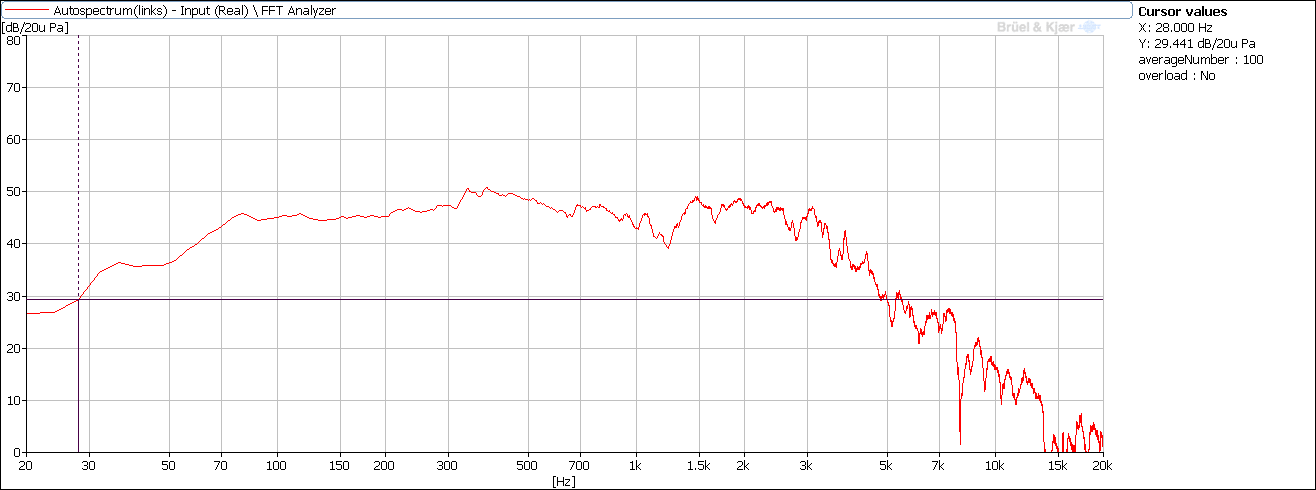
\includegraphics[width=1\textwidth]{img/LSMessung/TT/VisatonMitSilikonMitWolleV2.png}}
	\caption{Subwoofer-Messung mit Wolle\\ \enquote{Renkforce} (oben) und \enquote{Visaton} (unten) | Boxenvolumen: 149 l}
	\label{fig:4.2.3.3}
\end{figure}
Beide Frequenzgänge wurden durch das Hinzufügen von Wolle etwas \enquote{glatter}, also weisen weniger Welligkeit auf.
Die Wolle kann z.B. stehende Wellen in der Box verhindern und verbessert so die Eigenschaften der gesamten Box.\\ \\	%Es wirkt wie eine Vergrößerung des Volumens - hat Wagn einmal gsagt
Der Lautsprecher \enquote{Renkforce} weist insgesamt bei tieferen Frequenzen einen höheren Schalldruckpegel auf und wurde auch deshalb für dieses Projekt ausgewählt.

\newpage
\subsection*{Satelliten-Tiefton-Lautsprecher} \label{4.2.4}
Als Satelliten-Tiefton-Lautsprecher kommen mehrere Lautsprecher-Chassis in Frage, die vom Betreuer zu Verfügung gestellt wurden.
Die Lautsprecher-Chassis haben einen ähnlichen Durchmesser.
Dadurch können sie in einem Gehäuse (à 13,72 Liter) mit wechselbarer Frontplatte gemessen werden.
Um möglicherweise bessere Ergebnisse erzielen zu können wurde das Volumen mittels Ton-Ziegelstein, Styropor oder Ytong-Ziegel verringert, oder durch Wolle vergrößert.\\
Da das Gehäuse zu Beginn nicht komplett luftdicht abgeschlossen war, wurde es an den offenen Stellen mit Silikon verschlossen.
Um bei den wechselnden Frontplatten einen luftdichten Verschluss zu ermöglichen, wurde ein Gummi zwischen Gehäuse und Frontplatte verbaut.
Die Frontplatte wurden mittels Schrauben in der vorgesehenen Öffnung befestigt.\\ \\
Zu den gemessenen Chassis gehören:
\begin{itemize}
	\item \enquote{TT1}: PSS 297 58206 100W 6Ohm
	\item \enquote{TT2}: SAMCO 10D1K06 20W 8Ohm
%	\item \enquote{TT3}: Infinity, ein Auto-Lautsprecher
\end{itemize}
Die Bezeichnung TT1 und TT2 dient zur Vereinfachung.\\

%\newpage
Wie zuvor erwähnt wurden die Messungen zu Beginn der Diplomarbeit über einen Screenshot festgehalten.
Man wurde im Verlauf der Diplomarbeit auf eine bessere Methode zur Dokumentation hingewiesen, welche im Laufe der Messungen angewandt wurde.
Jene Verbesserung wird auf zwei Punkte bezogen:\\
\begin{enumerate}
	\item Die Skalierung der Y-Achse sollte von 0 bis 60 dB reichen, da diese Skalierung normalerweise für Lautsprechermessungen verwendet und so dieser Bereich genauer aufgelöst wird.
	\item Es sollte nur das Fenster des Frequenzganges gespeichert werden, um eine höhere Auflösung für diesen zu erhalten.
\end{enumerate}

\newpage
\textit{Die folgenden Messungen wurden bereits mit dem mit Silikon verschlossenen Gehäuse erstellt.}\\
\begin{figure} [H]
	\centering
	\subfloat{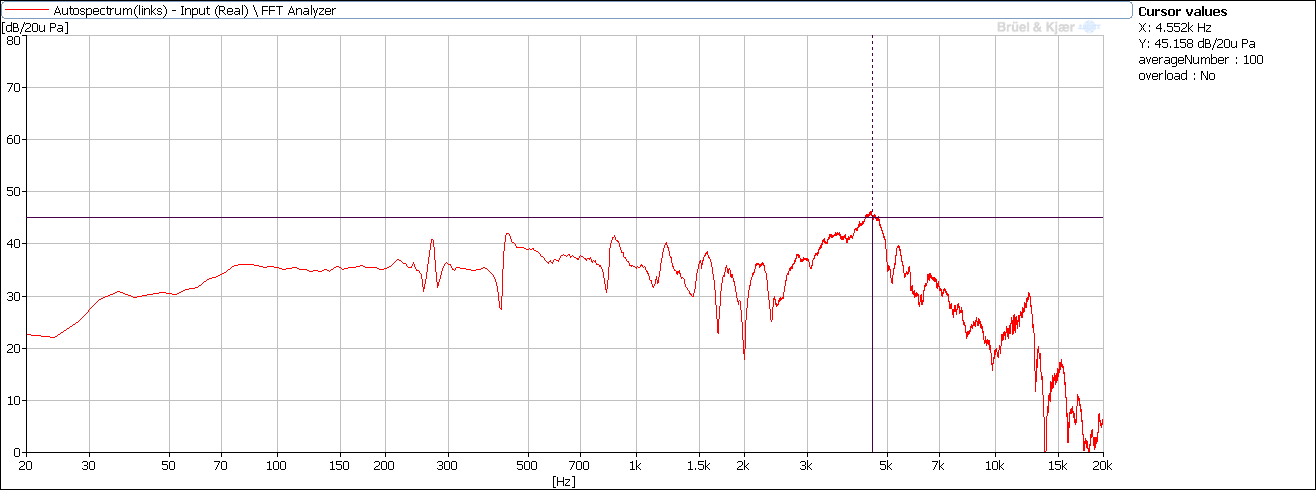
\includegraphics[width=1\textwidth]{img/LSMessung/TT/TT1mitSilikonV2.png}}\quad
	\subfloat{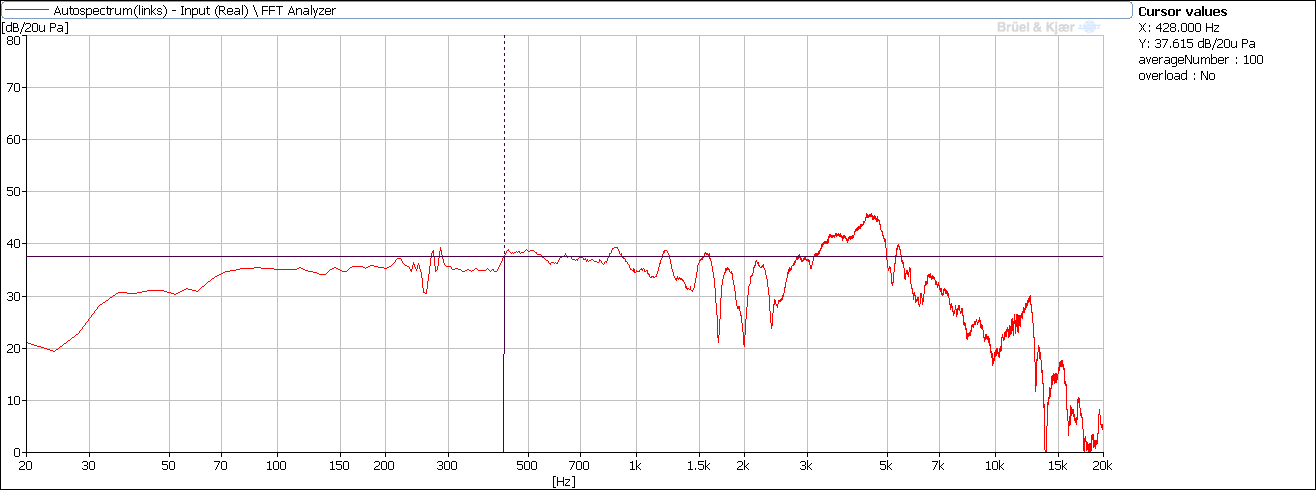
\includegraphics[width=1\textwidth]{img/LSMessung/TT/TT1mitSilikonUndWolleV2.png}}
	\caption{Tiefton-Lautsprecher-Messung ohne Wolle\\ \enquote{TT1} (oben) und mit Wolle \enquote{TT1} (unten) | Boxenvolumen: 13,72l}
	\label{fig:4.2.4.1}
\end{figure}
Es ist die Verringerung der Welligkeit im Tieftonbereich (<1 kHz) sichtbar.
In dieser Situation sollte der Tiefton-Lautsprecher im besten Fall bis 1 kHz arbeiten.
Des weiteren sollte er besser mit Wolle versehen werden.

\newpage
Als Referenz wird der Lautsprecher \enquote{TT2} gemessen. 
Ebenfalls einmal ohne und einmal mit Wolle im Gehäuse.
\begin{figure} [H]
	\centering
	\subfloat{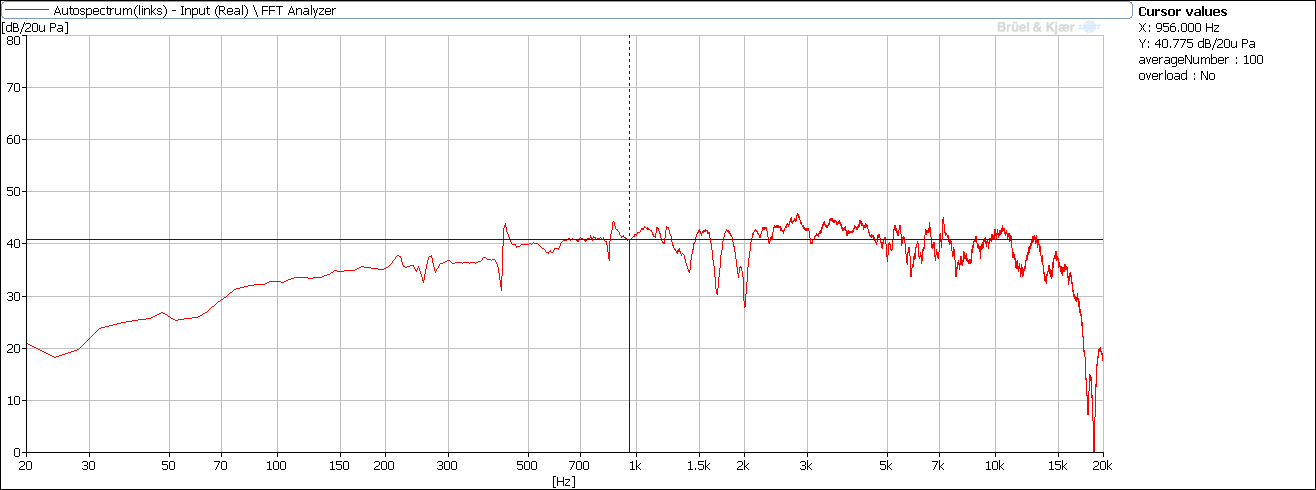
\includegraphics[width=1\textwidth]{img/LSMessung/TT/TT2mitSilikon_ohneWolleV2.png}}\quad
	\subfloat{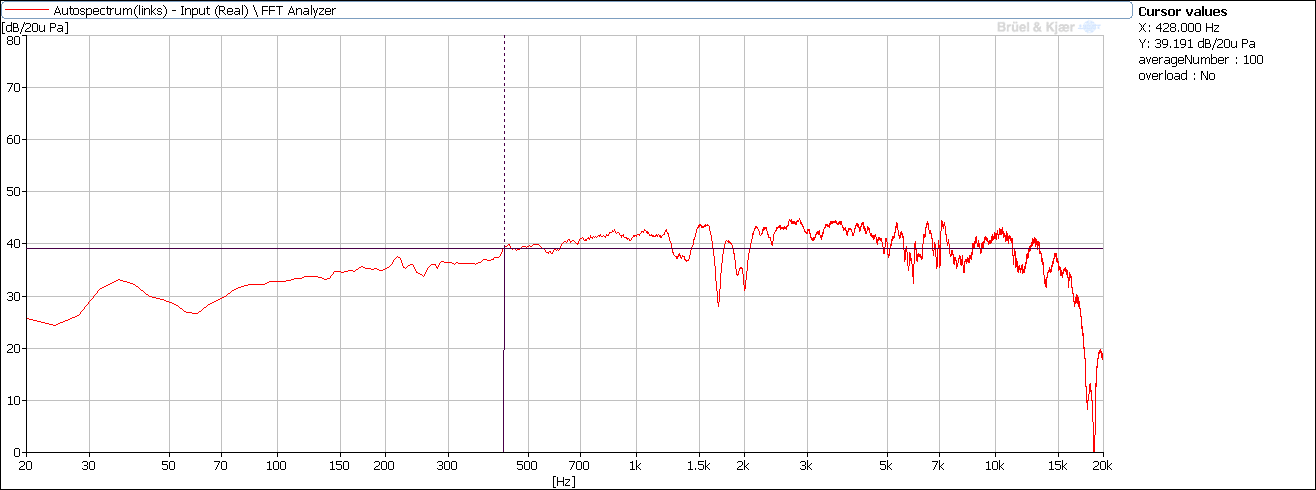
\includegraphics[width=1\textwidth]{img/LSMessung/TT/TT2mitSilikon_mitWolleV2.png}}
	\caption{Tiefton-Lautsprecher-Messung ohne Wolle\\ \enquote{TT2} (oben) und mit Wolle \enquote{TT2} (unten) Boxenvolumen: 13,72 l}
	\label{fig:4.2.4.2}
\end{figure}
Dieser Lautsprecher weist eine einigermaßen vertretbare Welligkeit im Mittel- und Hochton-Bereich auf.
Beim Niederton-Bereich ist der Schalldruckpegel jedoch geringer.
Der Mono-Subwoofer müsste bis einige 100 Hz aktiv sein, um diese Schwäche auszumerzen.
Ein Subwoofer sollte jedoch nicht über 150 bis 200 Hz kommen, da Frequenzen unterhalb dieser Grenze nicht lokalisiert werden können und, dass der Sinn eines Subwoofers wäre.
Wieder ist ersichtlich, dass mit Wolle die Welligkeit im Mittel und Tiefton-Bereich etwas verringert wird.

\newpage
Durch ein paar weitere Messungen wurde der TT2 bereits sehr früh aus der Auswahl genommen und der Fokus auf den TT1 gelegt, da dieser im Tieftonbereich besser funktioniert.
\\
Außerhalb der Messungen für die Diplomarbeit wurde der Lautsprecher TT1 etwas beschädigt.
Die \enquote{Dustcap} des Lautsprechers wurde eingedrückt.
Für einen Tiefton-Lautsprecher ist das nicht so schlimm, da die \enquote{Dustcap} in diesem Fall rein für den Schutz vor Staub zuständig ist.
Dies ist notwendig, um den Bewegungsfreiraum zwischen der Spule an der beweglichen Membran und der Spule am fixen Gehäuse gewährleisten zu können.
Wenn dieser Schutz nicht vorhanden ist, ist meist auch der Lautsprecher kaputt.\\
Bei einem Hochton-Lautsprecher wäre bereits das Eindrücken der \enquote{Dustcap} ein Todesurteil für den Lautsprecher, da die Halbkugelstruktur der \enquote{Dustcap} in diesem Frequenzbereich einen immensem Einfluss auf den Klang nimmt.
\\ \\
Nach Feststellen des Schadens wurde der Frequenzgang des TT1 erneut überprüft und er wies keine wesentlichen Veränderungen im Spektrum auf, was zu dem Schluss führte, dass er normal weiter verwendet werden kann.
\\

% IN KAPITEL OPTIMIERUNG !
%Als nächster Schritt werden die Tieftöner unter variierendem Volumen gemessen.
%Dafür wird, wie zuvor erwähnt, hauptsächlich Ytong und Styropor verwendet.
%Styropor gilt auch als einigermaßen schalltotes Material.
%Da keine fixen Angaben gemacht wurden was die Schalldichte von Styropor betrifft, wurde eine Referenzmessung mit Ziegeln gemacht(Siehe Kapitel \ref{label}). % Referenzmessung Styropor, Ziegel einbauen!
%\\
%Das Volumen wird zuerst einmal stark verringert, um zu sehen ob überhaupt ein Effekt merkbar ist.
%Dafür wird das Volumen von 13,72l auf 4,87l verringert.
%\begin{figure} [H]
%	\centering
%	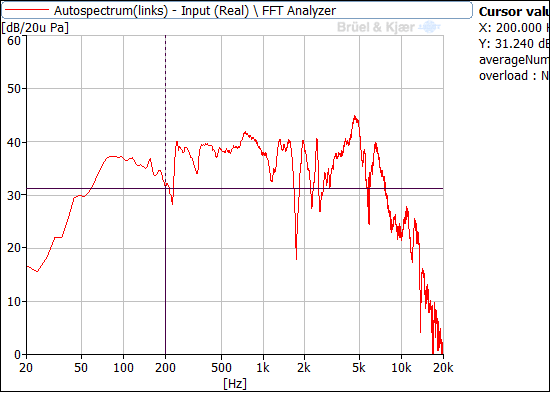
\includegraphics[width=0.7\textwidth]{img/LSMessung/TT/TT1silikon_4-87lVolumen.png}
%	\caption{\enquote{TT1} | Boxenvolumen = 4,87 l}
%	\label {fig:5.3.4.3}
%\end{figure}

%Vergleich mit original machen












%TD -- Kapitel 4.3 -- alle Labels darauf aufbauend

\newpage
\section{Lautsprecher für Hochton-Bereich}\label{sec:4.3}
Je ein Hochton-Lautsprecher wird in eine Satelliten-Box verbaut.
Während für die Tiefton-Lautsprecher das Volumen noch sehr wichtig ist, weil es den Frequenzgang des Lautsprechers beeinflussen kann, spielt das Volumen für die Hochton-Lautsprecher keine große Rolle mehr.
Dies ist bedingt dadurch, dass der Schall des Hochton-Lautsprecher sich hauptsächlich in Abstrahlrichtung der Membran ausbreitet.
%Das kommt daher, dass der Schall nur aus Richtung der Hochton-Lautsprecher-Membran abgestrahlt wird.
Die Box wird also durch hohe Töne nicht in Schwingung versetzt.
\\ \\
Folgende Hochton-Lautsprecher wurden gemessen:
\begin{itemize}
	\item TW203
	\item AE-1004
	\item Sharp 50T
	\item DT4810ASZR
	\item U2275
	\item Visaton DTW72 (zugekauft)
\end{itemize}
Um vergleichbare Messungen zu erhalten, wurden alle Hochton-Lautsprecher mit einer Entfernung von 1 m zum Mikrofon gemessen.
Außerdem wurden alle Lautsprecher in einer Höhe von 1 m platziert, um Reflexionen mit dem Boden des Messraums zu verhindern.
Vor allem aus dem Grund, da es sich bei dem Boden um ein Metallgitter handelt.
In den Auslassungen des Gitters könnte es zu möglichen Resonanzen oder Reflexionen kommen, die das Messergebnis verfälschen.
\newpage

\begin{figure} [H]
	\centering
	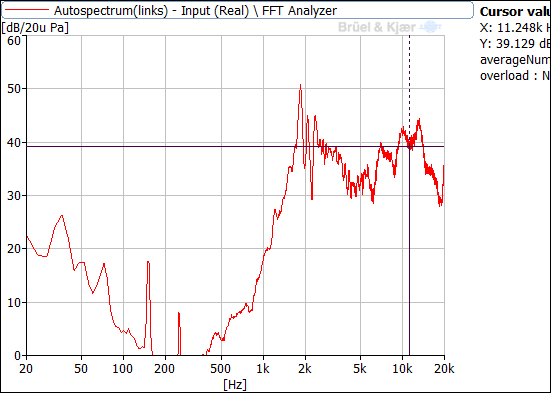
\includegraphics[width=0.8\textwidth]{img/LSMessung/HT/TW203_1m_erhoeht.png}
	\caption{Frequenzgang \enquote{TW203}}
	\label{fig:4.3.1}
\end{figure}

\begin{figure} [H]
	\centering
	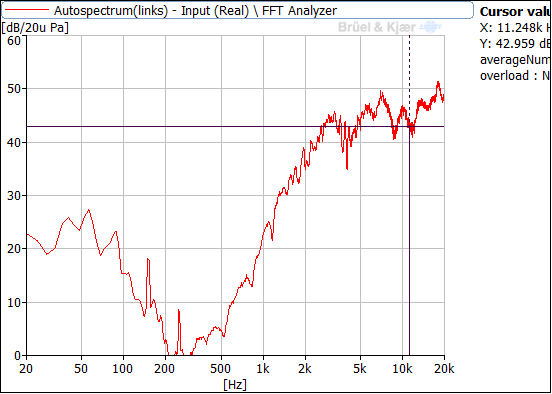
\includegraphics[width=0.8\textwidth]{img/LSMessung/HT/AE1004_1m_erhoeht.png}
	\caption{Frequenzgang \enquote{AE-1004}}
	\label{fig:4.3.2}
\end{figure}

\begin{figure} [H]
	\centering
	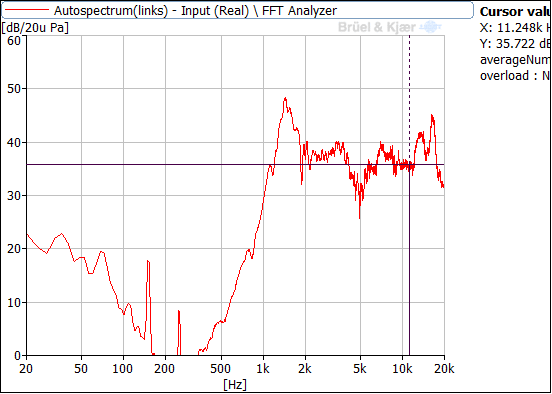
\includegraphics[width=0.8\textwidth]{img/LSMessung/HT/Sharp_1m_erhoeht.png}
	\caption{Frequenzgang \enquote{Sharp 50T}}
	\label{fig:4.3.3}
\end{figure}

\begin{figure} [H]
	\centering
	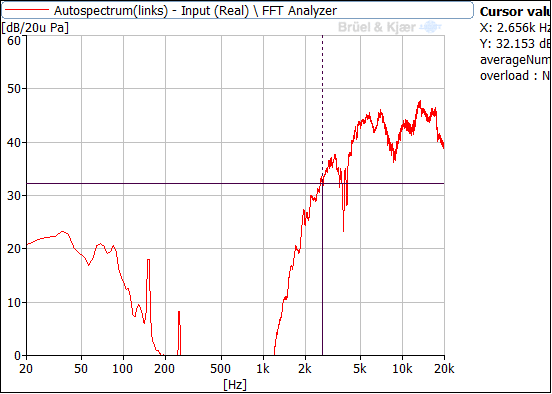
\includegraphics[width=0.8\textwidth]{img/LSMessung/HT/DT4810ASZR_1m_erhoeht.png}
	\caption{Frequenzgang \enquote{DT4810AZSR}}
	\label{fig:4.3.4}
\end{figure}

\begin{figure} [H]
	\centering
	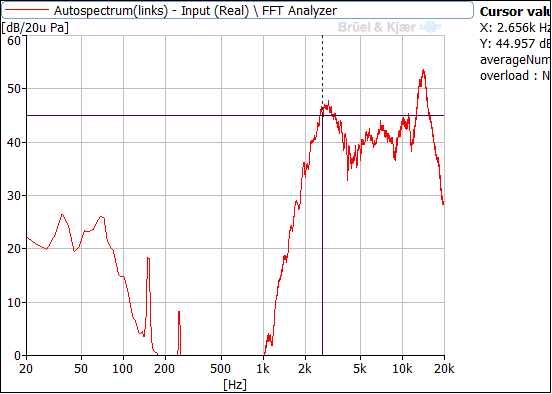
\includegraphics[width=0.8\textwidth]{img/LSMessung/HT/U2275_1m_erhoeht.png}
	\caption{Frequenzgang \enquote{U2275}}
	\label{fig:4.3.5}
\end{figure}

\begin{figure} [H]
	\centering
	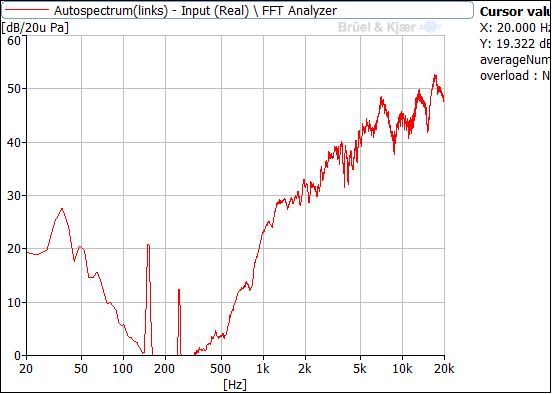
\includegraphics[width=0.8\textwidth]{img/LSMessung/HT/VisatonDTW72.png}
	\caption{Frequenzgang \enquote{Visaton DTW72}}
	\label{fig:4.3.6}
\end{figure}
\newpage
Im Bereich unter 500 Hz sind bei den Messungen relativ hohe Pegel aufgetreten.
In diesem Frequenzbereich kann ein Hochton-Lautsprecher aber nicht solche Schalldruckpegel erzeugen, dafür ist die Membranfläche zu klein.
Daraus ist zu schließen, dass diese Pegel durch verschiedene Störeinflüsse auf die Messung erzeugt wurden.
Diese Einflüsse könnten sein: Beeinflussung der Messung durch das 50 Hz Stromnetz, äußere Einflüsse auf den nahezu schalldichten Raum (Trittschall), usw.
\\ \\
Da viele dieser gemessenen Frequenzgänge eine hohe Welligkeit oder erst bei relativ hohen Frequenzen einen angemessenen Schalldruckpegel aufweisen, wurde von uns der Hochton-Lautsprecher \enquote{Visaton DTW72} (Frequenzgang: Abb. \ref{fig:4.3.6}) zugekauft und für das Projekt ausgewählt.
\\ \\
Dieser Lautsprecher weist einen angemessenen Schalldruckpegel bei relativ geringer Welligkeit auf und ist daher optimal.
Außerdem könnte er bereits ab ca. 1 kHz verwendet werden.

\begin{figure} [H]
	\centering
	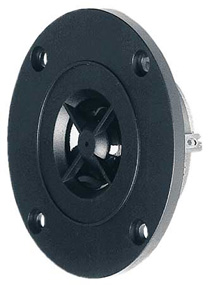
\includegraphics[width=0.4\textwidth]{img/LSMessung/HT/dtw72.jpg}
	\caption[Lautsprecher \enquote{Visaton DTW72}]{Lautsprecher \enquote{Visaton DTW72}\footnotemark}
	\label{fig:4.3.7}
\end{figure}
\footnotetext{http://www.visaton.de/de/chassis\_zubehoer/ht\_kalotten/dtw72\_8.html,\\Zugriff: 13.03.2017}
%http://www.visaton.de/de/chassis_zubehoer/ht_kalotten/dtw72_8.html

%TD Generelle Messung des Equipments aus dem Word "20170107-SubwooferMessungen.docx" einbauen?

% ^ -> Ich würde wenn dann nur schreiben, dass das Equipment getestet wurde und alles top war!

\newpage
\section{Optimierung der Lautsprecher-Boxen}\label{sec:4.4}
Die ausgewählten Lautsprecher-Chassis sind hier noch einmal zusammengefasst:
\begin{itemize}
	\item Subwoofer: \enquote{Renkforce B12123}
	\item Tiefton-Lautsprecher (2x): \enquote{PSS 297 58206}
	\item Hochton-Lautsprecher (2x): \enquote{Visaton DTW72}
\end{itemize}
Um nun den optimalen Klang bzw. das optimale Boxenvolumen für Satelliten-Boxen sowie Subwoofer-Box herauszufinden, werden weitere Messungen durchgeführt.
Das Volumen der Boxen wird dabei verringert, um so das kleinste Volumen bei gleichzeitig noch hohem Pegel und geringer Welligkeit zu finden.

\subsection{Eignung von verschiedenen Materialien zur Volumsverminderung}\label{subsec:4.4.1}
Zur Verringerung des Volumens der Subwooferbox wird eine große Menge an schalldichtem Material benötigt.
Da Ton-Ziegelsteine sehr schwer und nicht ausreichend vorhanden sind, wird eine Vergleichsmessung mit Styropor angestellt, um zu belegen, dass sich dieses Material ebenfalls zur Volumsverminderung eignet.
% I würd des goa ned erwähnen ;)
Um die Messungen vergleichen zu können, wird die aufgenommene Kurve aus \enquote{PULSE LabShop} in eine Zusatzapplikation dieser Software geladen.
Dabei handelt es sich um die Kalkulationssoftware von \enquote{PULSE LabShop}.
Um die Kurven in ein Diagramm zusammenzufügen, muss zuerst jede Messung als 
Textdatei gespeichert werden.
In dieser Datei stehen die für die Berechnung relevanten Daten jedes einzelnen Punktes in der Kurve.
Nach dem Speichern jeder Kurve können diese Daten in die Berechnungssoftware geladen werden.
Die Software beherrscht einige mathematische Funktionen.
Unter anderem kann man die Differenz zwischen zwei Kurven ermitteln.\\ 
Für diese Messungen wird der \enquote{TT1} und die 13,72 l Box herangezogen.
Es wurde grundsätzlich in zwei Messbereiche unterteilt.
Von 20 Hz bis 20 kHz, das ganze Audiospektrum, und von 20 Hz bis 500 Hz, da in diesem Bereich eine Volumsverminderung deutliche Unterschiede hervorbringen kann.
Es wurden drei Kurven aufgenommen und verglichen.\\
Diese waren:
\begin{itemize}
	\item Volumsverminderung mit Ytong-Ziegel
	\item Volumsverminderung mit Styropor
	\item ohne Volumsverminderung
\end{itemize}
Das Volumen wurde jeweils um 4,5 l vermindert.
Zwischen den Kurven von Styropor und Ytong-Ziegel wurde zusätzlich die Differenz gebildet.

\begin{figure} [H]
	\centering
	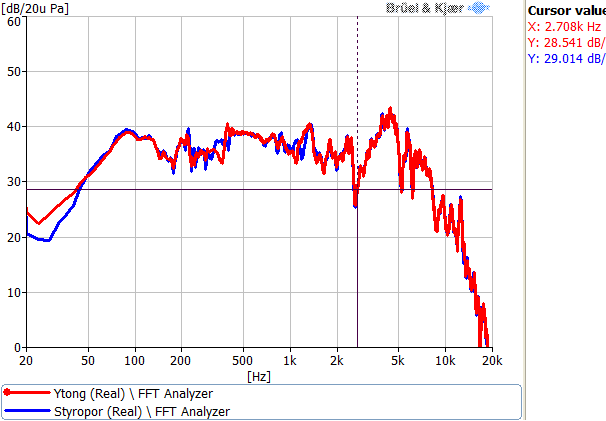
\includegraphics[width=0.75\textwidth]{img/Optimierung/Vergleich/VergleichYtognStyro_full.png}
	\caption{Vergleichsmessung Styropor zu Ytong-Ziegel von 20 Hz bis 20 kHz}
	\label{fig:4.4.1.1}
\end{figure}
\begin{figure} [H]
	\centering
	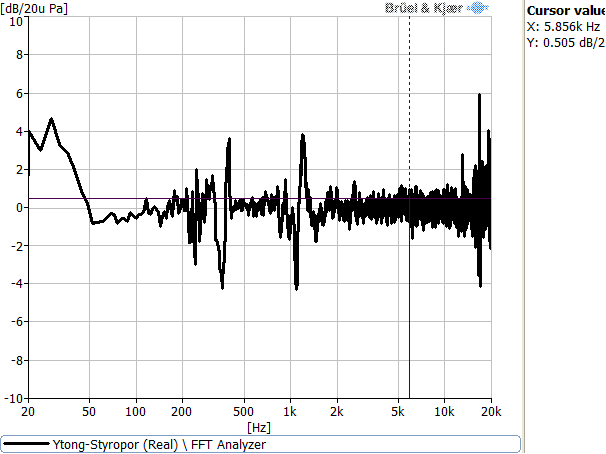
\includegraphics[width=0.75\textwidth]{img/Optimierung/Vergleich/VergleichYtognStyro_Abweichung_full.png}
	\caption{Vergleichsmessung Styropor zu Ytong-Ziegel von 20 Hz bis 20 kHz - Differenz der beiden Kurven}
	\label{fig:4.4.1.2}
\end{figure}


\begin{figure} [H]
	\centering
	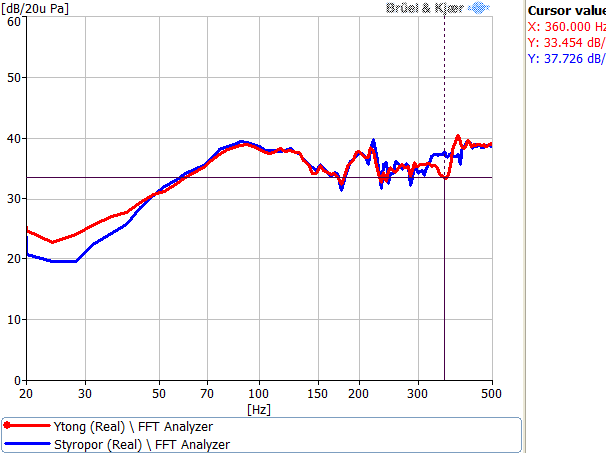
\includegraphics[width=0.75\textwidth]{img/Optimierung/Vergleich/VergleichYtognStyro_500Hz.png}
	\caption{Vergleichsmessung Styropor zu Ytong-Ziegel von 20 Hz bis 500 Hz}
	\label{fig:4.4.1.3}
\end{figure}
\begin{figure} [H]
	\centering
	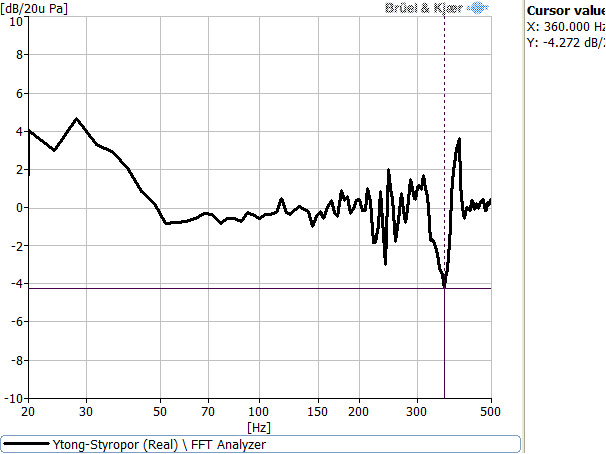
\includegraphics[width=0.75\textwidth]{img/Optimierung/Vergleich/VergleichYtognStyro_Abweichung_500Hz.png}
	\caption{Vergleichsmessung Styropor zu Ytong-Ziegel von 20 Hz bis 500 Hz - Differenz der beiden Kurven}
	\label{fig:4.4.1.4}
\end{figure}


\begin{figure} [H]
	\centering
	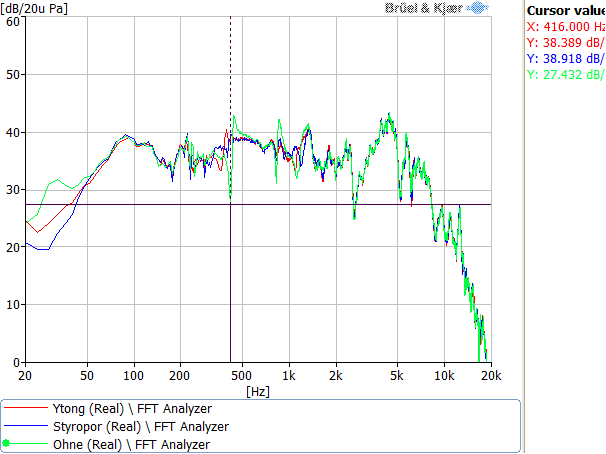
\includegraphics[width=0.75\textwidth]{img/Optimierung/Vergleich/VergleichYtognStyroOhne_full.png}
	\caption{Vergleichsmessung Styropor zu Ytong-Ziegel zu ohne Verminderung, von 20 Hz bis 20 kHz}
	\label{fig:4.4.1.5}
\end{figure}\begin{figure} [H]
	\centering
	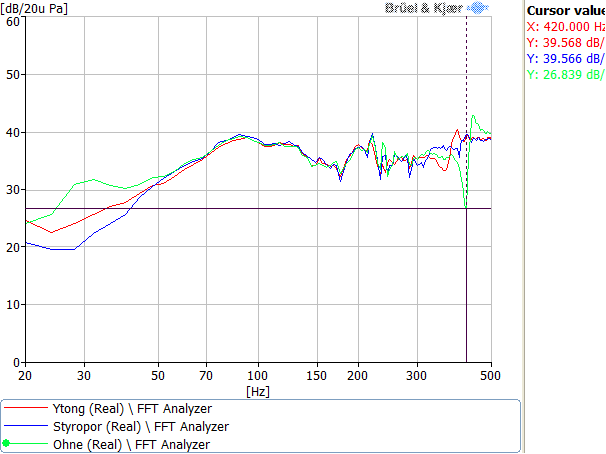
\includegraphics[width=0.75\textwidth]{img/Optimierung/Vergleich/VergleichYtognStyroOhne_500Hz.png}
	\caption{Vergleichsmessung Styropor zu Ytong-Ziegel zu ohne Verminderung, von 20 Hz bis 500 Hz}
	\label{fig:4.4.1.6}
\end{figure}

Die Schlussfolgerung aus diesen Messungen ist, dass Styropor sich auch zur Volumsverminderung von Lautsprechern gut eignet.
Aus diesem Grund wird Styropor auch hauptsächlich bei den folgenden Messungen verwendet.
\\ \\




\subsection{Subwoofer-Box}\label{subsec:4.4.2}
Das Ziel ist, die Box so klein wie möglich zu bauen, ohne Verlust an Klangqualität und Pegel.
Dafür wird die Messbox mit 149 l in ihrem Volumen vermindert, um zu testen, ob zuvor genannte Verluste auftreten.
Zu Beginn wird das Volumen drastisch verkleinert, in diesem Fall von 149 l auf 47,4 l (Bild \ref{fig:4.4.2.1}).

\begin{figure} [H]
\centering
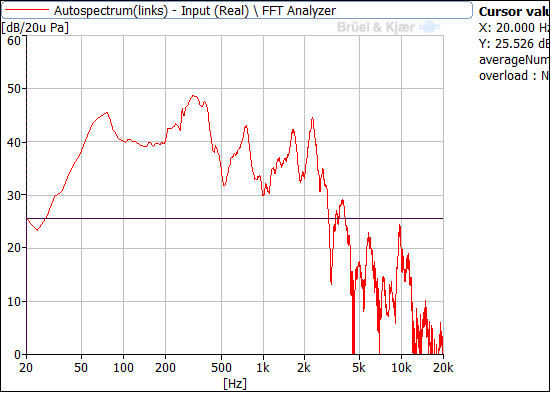
\includegraphics[width=0.75\textwidth]{img/Optimierung/Sub/RenkforceStyro_47l.png}
\caption{Renkforce Subwoofer: Styropor \\Volumen = 47,4 l}
\label{fig:4.4.2.1}
\end{figure}

Die folgenden Messungen mit verschiedenen Volumina wurden an einem anderen Messtag erstellt.
In der Zwischenzeit wurden von anderen Personen ebenfalls Messungen erstellt, wobei das Verstärkerlevel des Messverstärkers verändert wurde.
Im ersten Moment wurde diese Änderung übersehen, jedoch nach Bemerken wieder an die einheitliche Messeinstellung angepasst.
Die vor Änderung aufgenommenen Kurven weisen einen um 8dB höheren Pegel auf als die danach aufgenommenen Kurven.
Um zu bestätigen, dass nicht die Volumsverminderung Schuld an der Pegeländerung ist, wurde eine Vergleichsmessung mit einem zuvor gemessenen Volumen angestellt.\\

\textit{\textbf{ Die folgenden Messaufnahmen weisen einen um 8dB erhöhten Pegel auf.}} Dazu gehören: Messung \ref{fig:4.4.2.2}, \ref{fig:4.4.2.3}, \ref{fig:4.4.2.4} und \ref{fig:4.4.2.5}\\

\begin{figure} [H]
\centering
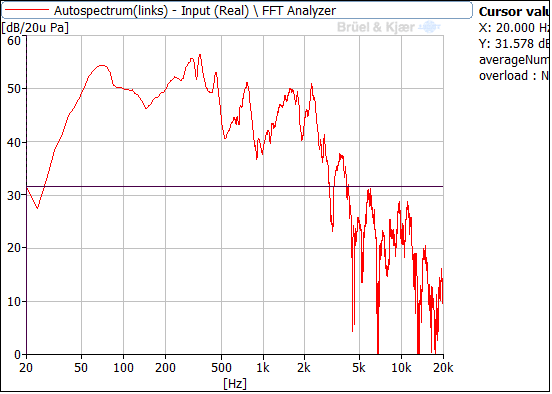
\includegraphics[width=0.74\textwidth]{img/Optimierung/Sub/RenkforceStyro_138l.png}
\caption{Renkforce Subwoofer: Styropor \\Volumen = 138,28 l}
\label{fig:4.4.2.2}
\end{figure}

\begin{figure} [H]
\centering
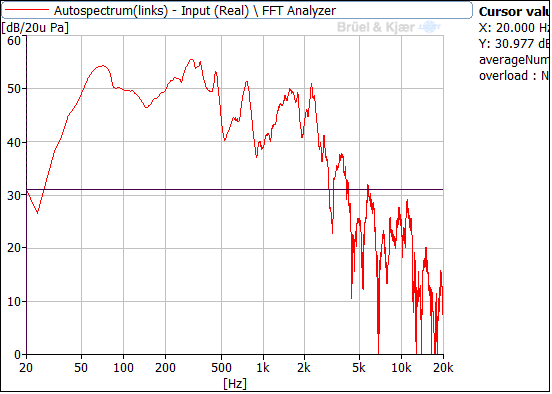
\includegraphics[width=0.74\textwidth]{img/Optimierung/Sub/RenkforceStyro_138l_Wolle.png}
\caption{Renkforce Subwoofer: Styropor, mit Wolle \\Volumen = 138,28 l}
\label{fig:4.4.2.3}
\end{figure}

\begin{figure} [H]
\centering
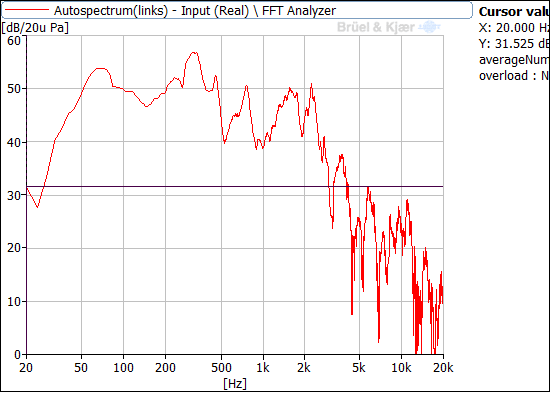
\includegraphics[width=0.75\textwidth]{img/Optimierung/Sub/RenkforceStyro_126l_Wolle.png}
\caption{Renkforce Subwoofer: Styropor, mit Wolle \\Volumen = 126,51 l}
\label{fig:4.4.2.4}
\end{figure}

\newpage
\textit{Die folgenden Messungen zeigen den Vergleich von verstellter Ausgangsverstärkung zu einheitlich verwendeten Ausgangsverstärkung. (Bild \ref{fig:4.4.2.5} und \ref{fig:4.4.2.6})}
\begin{figure} [H]
\centering
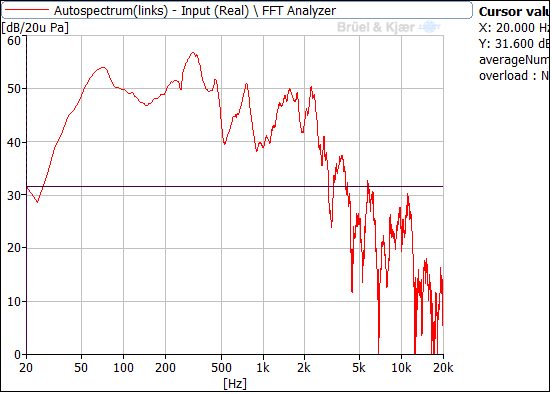
\includegraphics[width=0.65\textwidth]{img/Optimierung/Sub/RenkforceStyro_113l_Wolle.png}
\caption{Renkforce Subwoofer: Styropor und Ytong-Ziegel, mit Wolle \\Volumen = 113,25 l}
\label{fig:4.4.2.5}
\end{figure}

\begin{figure} [H]
\centering
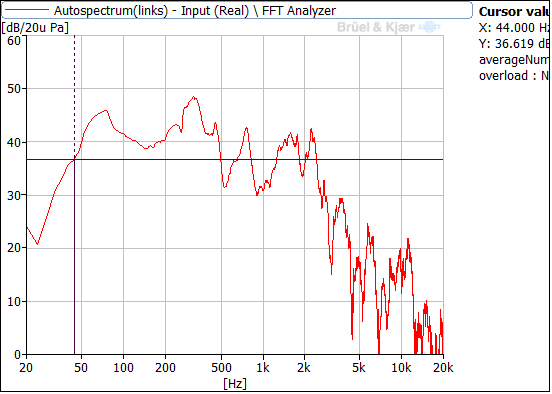
\includegraphics[width=0.65\textwidth]{img/Optimierung/Sub/RenkforceStyro_113l_Wolle_Angepasst.png}
\caption{Renkforce Subwoofer: Styropor und Ytong-Ziegel, mit Wolle - Angepasster Pegel \\Volumen = 113,25 l}
\label{fig:4.4.2.6}
\end{figure}
Beim Vergleich der beiden Kurven (Abb. \ref{fig:4.4.2.5 } \& \ref{fig:4.4.2.6}) ist lediglich eine Verschiebung auf der Y-Achse merkbar.

\newpage
Nach den vielen verschiedenen Messungen, konnte der Schluss gezogen werden, dass ein Innenvolumen der Box von 47 Liter ausreicht, um die gleiche Klangqualität unter dem selben Schalldruckpegel zu erreichen.\\
Ein kleineres Volumen wurde nicht angestrebt, da die ganze Elektronik ( Verstärker, Weichen, Akku, ...) ebenfalls in der Box Platz haben soll.
Aus diesem Grund wird eine Box mit einem Innenvolumen von 50 Litern angestrebt.\\ \\ \\ \\




\subsection{Box für Satelliten-Boxen}\label{subsec:4.4.3}
Gleich wie für die Subwoofer-Box, gilt auch hier das Boxenvolumen weitestgehend zu vermindern, unter der Bedingung, dass Klangqualität und Schalldruckpegel nicht darunter leiden.
Hier wird die Tiefton-Lautsprecher-Box mit 13,72 l als Messbox verwendet.
Mit verschiedenen Volumina und mit oder ohne Wolle wird das Tiefton-Lautsprecher-Chassis \enquote{TT1} gemessen.\\
Zuallererst wird der Extremvergleich angestellt.
Die Messung \ref{fig:4.4.3.1} wurde ohne Styropor und ohne Wolle aufgenommen.
Im Vergleich zu dieser steht die Messung \ref{fig:4.4.3.2}.
Diese wurde mit einem durch Styropor verringerten Volumen gemessen, sodass die Box ein Innenvolumen von 4,87 l hatte.

\newpage
\begin{figure} [H]
	\centering
	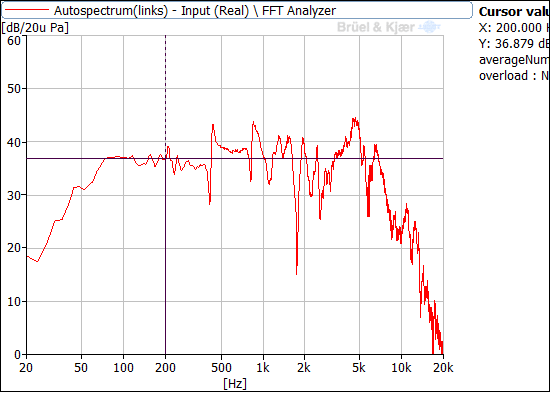
\includegraphics[width=0.75\textwidth]{img/Optimierung/TT/TT1_ohneAllem.png}
	\caption{PSS 297 58206 (\enquote{TT1}) ohne Volumsverminderung \\Volumen = 13,72 l}
	\label{fig:4.4.3.1}
\end{figure}

\begin{figure} [H]
	\centering
	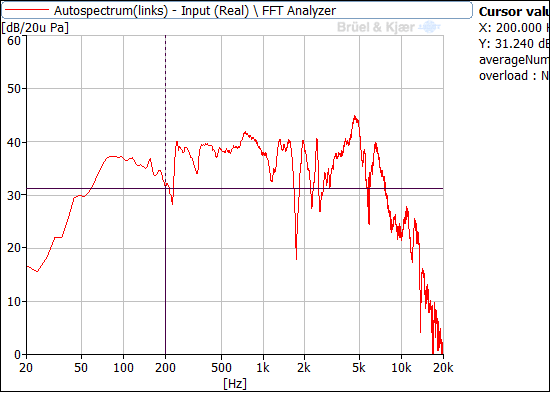
\includegraphics[width=0.75\textwidth]{img/Optimierung/TT/TT1_Styro_4-87l.png}
	\caption{PSS 297 58206 (\enquote{TT1}) Volumsverminderung durch Styropor \\Volumen = 4,87 l}
	\label{fig:4.4.3.2}
\end{figure}

%TD Bitte Korregieren falls ich mich vertan habe!
\newpage
Als nächstes wurde versucht, den Einbruch in der Frequenzgangskurve bei 1.75 kHz zu verhindern.
Ein möglicher Grund für diesen Einbruch kann eine Resonanz in der Box aufgrund der Seitenwandlänge sein.
Diese Annahme kommt daher, dass die Seitenlänge der Box relativ lang ist und möglicherweise genau $\frac{\lambda}{2}$ für den verwendeten Frequenzbereich bedeutet und dadurch die an der Rückwand reflektierte Welle mit der hin laufenden Welle interferiert.
Es entsteht eine Resonanz mit der Box.
Es wird deshalb eine Schraubzwinge mittig der Seitenwand auf der Box montiert, um die mögliche Resonanz zu unterbinden.
%WAtch here please!
%Durch das anbringen der Schraubzwinge wird die Seitenwand in der Mitte stabiler, teilt daher die Seitenlänge in der Mitte und verhindert so das Mitschwingen der Wand für die Frequenz resultierend aus der Länge.
Als Vergleich wird die Messung mit selbigen Volumsbedingungen und ohne Schraubzwinge herangezogen (Bild \ref{fig:4.4.3.1}).
Die Messung mit Schraubzwinge ergibt aber keinen wesentlichen Unterschied (Bild \ref{fig:4.4.3.3}).\\ \\

\begin{figure} [H]
	\centering
	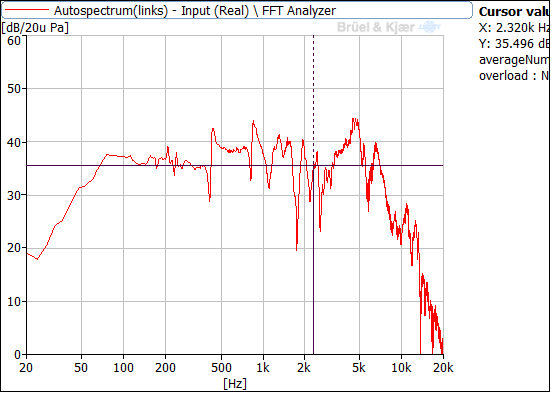
\includegraphics[width=0.75\textwidth]{img/Optimierung/TT/TT1_ohneAllem_Schraubzwinge.png}
	\caption{PSS 297 58206 (\enquote{TT1}) ohne Volumsverminderung, mit Schraubzwinge \\Volumen = 13,72 l}
	\label{fig:4.4.3.3}
\end{figure}

\newpage
Nachfolgend wurden weitere Kurven unter Volumsänderung aufgenommen.

\begin{figure} [H]
	\centering
	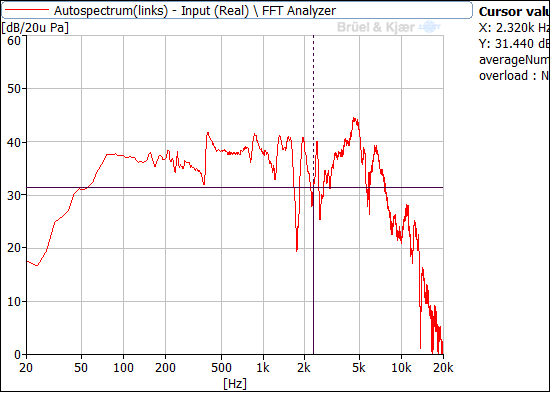
\includegraphics[width=0.75\textwidth]{img/Optimierung/TT/TT1_Styro_9-67l.png}
	\caption{PSS 297 58206 (\enquote{TT1}) ohne Volumsverminderung \\Volumen = 9,67 l}
	\label{fig:4.4.3.4}
\end{figure}

\begin{figure} [H]
	\centering
	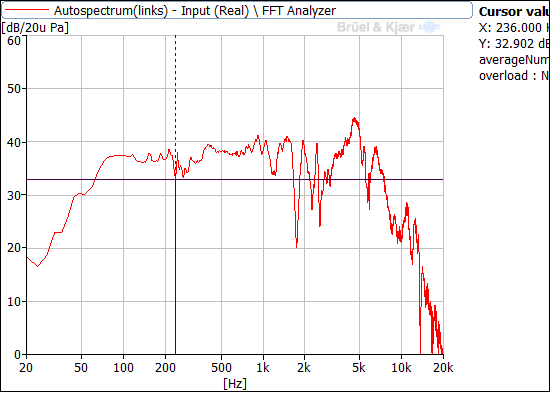
\includegraphics[width=0.75\textwidth]{img/Optimierung/TT/TT1_Styro_7-17l.png}
	\caption{PSS 297 58206 (\enquote{TT1}) ohne Volumsverminderung \\Volumen = 7,17 l}
	\label{fig:4.4.3.5}
\end{figure}

\begin{figure} [H]
	\centering
	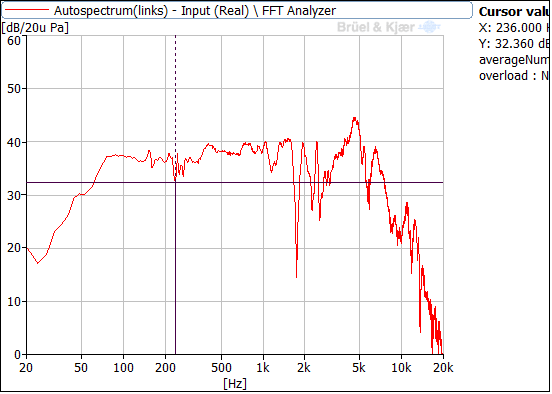
\includegraphics[width=0.7\textwidth]{img/Optimierung/TT/TT1_Styro_6-07l.png}
	\caption{PSS 297 58206 (\enquote{TT1}) ohne Volumsverminderung \\Volumen = 6,07 l}
	\label{fig:4.4.3.6}
\end{figure}

\begin{figure} [H]
	\centering
	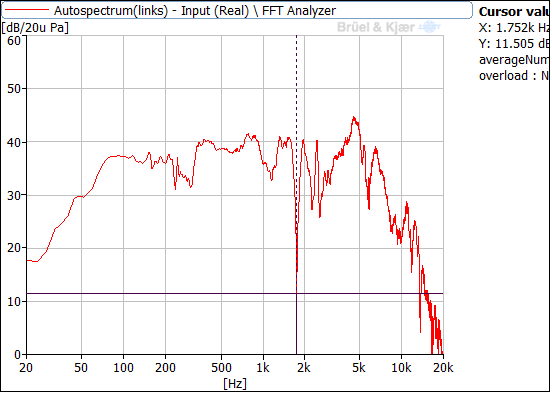
\includegraphics[width=0.7\textwidth]{img/Optimierung/TT/TT1_Styro_5-47l.png}
	\caption{PSS 297 58206 (\enquote{TT1}) ohne Volumsverminderung \\Volumen = 5,47 l}
	\label{fig:4.4.3.7}
\end{figure}

\textbf{Schlussendlich erschien die Messkurve \ref{fig:4.4.3.5} als beste Kurve, da sie in einem Bereich von ungefähr 60 Hz bis 1,7 kHz eine sehr geringe Welligkeit aufweist (> +/- 5dB).
Aus diesem Grund wird ein Satelliten-Boxen-Volumen von 7 Liter angestrebt.}



% Technische Erklärung der Prints
\chapter{Entwicklung der Elektronik-Platinen}
%\newpage
\section{Verstärker-Schaltungen}

\subsection{Verstärker für Hochton-Bereich}

\subsection{Verstärker für Tiefton-Bereich}

\subsection{Subwoofer-Verstärker}


\section{Frequenzweichen}


\section{Beschaltung des Bluetooth-Moduls}

\responsible{Markus Bointner}
\section{Verstärker-Schaltungen}


\subsection{Verstärker für Hochton-Bereich}
\subsubsection{Allgemeines}\label{subsec:4.5.1}
Die gefilterten Hochton-Frequenzen müssen vor dem Abstrahlen verstärkt werden.
Hierfür wird die TDA2030-Verstärker-Grundschaltung(siehe Kapitel \ref{subsec:3.2.2}) verwendet.
%TDA2030 Grundschaltung Verweis
Hier ohne Leistungstransistoren, da Hochton-Lautsprecher nicht eine so hohe Leistung ohne Gefahr von Zerstörung umsetzen können.
Die Spulen des Lautsprechers könnten bei zu hoher Leistung durchbrennen, d.h. der Isolierschutzlack der Spulenwindungen wird zu heiß, die Windungen werden kurzgeschlossen.
Das verstärkte Audiosignal weißt dadurch am Ausgang der Schaltung eine höhere Spannungs-Amplitude und einen höheren Strom auf.
Es soll nach diesem Schritt möglich sein den Hochton-Lautsprecher in einer der zwei Satellitenboxen mit ausreichend Signal zu versorgen, um einen Schalldruck von zumindest Zimmerlautstärke zu erhalten. 
% Sollen wir hier genau das selbe schreiben wie beim TTVerstärker?


\subsubsection{Schaltung}\label{subsec:4.5.2}
Aus der TDA2030-Grundschaltung (siehe Kapitel \ref{subsec:3.2.2}) folgend ist auch hier ein Spannungsteiler vorgesehen um den Arbeitspunkt (Siehe Kapitel \ref{subsec:3.5.1}) einzustellen.
%TDA2030 Grundschaltung Verweis + Arbeitspunkt Verweis
Die Schaltung wurde aus dem Datenblatt übernommen, nur vereinzelte Werte wurden angepasst. 
% Veränderte Werte nennen?

\begin{figure} [H]
	\centering	
	\includegraphics[width=1\textwidth]{img/Print6/HTVerstaerker-Schem.PNG}
	\caption{Verstärker für Hochton-Bereich - Schaltung}
	\label {fig:4.5.2.1}
\end{figure}


\subsubsection{PCB}\label{subsec:4.5.3}
Das Layout wird wieder nach den Grunddesignregeln(siehe Kapitel \ref{subsec:3.1.2}) erstellt.\\
%TD Grunddesignregel Verweis
Eine große Fläche über dem TDA2030 wird vorgesehen um einen Testkühlkörper mit dem Print mechanisch verbinden zu können.
Es dient zur Verringerung der Hebelwirkung.
%Mit Fortschreiten der Arbeit wurde die Fläche gekürtzt um mit dem neuen Kühlkörper eben abzuschließen.

\begin{figure} [H]
	\centering	
	\includegraphics[width=0.7\textwidth]{img/Print6/HTVerstaerker-PCB.PNG}
	\caption{Verstärker für Hochton-Bereich - PCB}
	\label {fig:4.5.3.1}
\end{figure}


\newpage
\subsection{Verstärker für Tiefton-Bereich}
\subsubsection{Allgemeines}\label{subsec:4.4.1}
Nach dem Filtern des Signals soll dieses vor dem Abstrahlen am Lautsprecher verstärkt werden.
Es wurde eine analoge Verstärker-Schaltung verwendet, da diese einfacher und mit weniger Problemen realisiert werden konnte.
Mithilfe bereits bekannter, bewährter Schaltungen konnte ein Layout für diese Schaltung designet werden.
Ein wichtiger Baustein in dieser Schaltung ist der Verstärkerbaustein \enquote{TDA2030} (Siehe Kapitel \ref{sec:3.2}).
%TDA2030 Verweis
Des weiteren werden zwei Leistungstransistoren verbaut die höhere Ströme schalten können, falls der maximale Schaltstrom des TDA2030 erreicht wird. (Siehe Kapitel \ref{subsec:3.2.3})
%TDA2030 MaxRatings
Das Eingangssignal soll verstärkt werden um am Ausgang der Schaltung höhere Spannungs-Amplituden und höheren Ströme aufzuweisen.
Es soll nach diesem Schritt möglich sein den Tiefton-Lautsprecher in einer der zwei Satellitenboxen mit ausreichend Signal zu versorgen, um einen Schalldruck von zumindest Zimmerlautstärke zu erhalten. 
%TD TDA2030 Verweis
%TD TDA2030-Maximum-Ratings Verweis

\subsubsection{Schaltung}\label{subsec:4.4.2}
In der linken, oberen Ecke der Schaltung (\ref{fig:4.4.2.1}) ist der Spannungsteiler für einstellen des Arbeitspunktes (Siehe Kapitel \ref{subsec:3.5.1}) ersichtlich.
Mit Hilfe des ELKO's \enquote{EL504} wird verschleppte Gleichspannung am Eingang der Schaltung heraus gesiebt.
Dafür ist auch der ELKO \enquote{EL502}, dieser siebt die Gleichspannung am Ausgang der Schaltung heraus, bevor das Signal die Platine verlässt. \\
Über die Widerstände \enquote{R506} und \enquote{R505} wird die Verstärkung der Schaltung eingestellt.
In diesem Fall ist die Verstärkung $\frac{R505+R506}{R505}$ = 31 .
Das bedeutet, dass das Eingangssignal am Ausgang 31mal so groß sein soll, natürlich unter Beachtung der Grenzen der OPV-Verstärkerschaltung (\ref{sec:3.5}).
%TD Arbeitspunkt Verweis
%TD OPV-Verstärkerschaltung Verweis
%TD Layout TT-Verst

\begin{figure} [H]
	\centering	
	\includegraphics[width=1\textwidth]{img/Print5/5_TTVerstaerker-Schem.PNG}
	\caption{Verstärker für Tiefton-Bereich - Schaltung}
	\label {fig:4.4.2.1}
\end{figure}


\subsubsection{PCB}\label{subsec:4.4.3}
Die drei zu kühlenden Bauteile \enquote{Q502, U501, Q501} (\ref{fig:4.4.3.1}) sind auf selber Höhe montiert um sie auf einen Kühlkörper montieren können.
\emph{Zu beachten dabei ist deren Potential an der Kühlfläche!}
Das Potential ist das Selbe wie an dem mittleren Anschluss-Pin des jeweiligen Bauteils.
Daher:
\begin{itemize}
	\item TDA2030: \enquote{-Vcc} = Masse bei asymmetrische Versorgung
	\item PNP(Q501): \enquote{Kollektor} = Ausgangssignal TDA2030
	\item NPN(Q502): \enquote{Kollektor} = Ausgangssignal TDA2030
\end{itemize}

Aus diesem Grund müssen zumindest die zwei Transistoren isoliert am Kühlkörper angebracht werden.\\
Die Ein- und Ausgänge sind auf einer Seite montiert. 
Einheitlich mit der Hochtonverstärkerplatine(\ref{sec:4.5}) ist von links nach rechts zuerst Versorgungsstecker, dann Eingangssignal und am Ende der Ausgangsstecker angebracht.
Ebenso ist Masse jeweils rechts angeordnet um die Einheitlichkeit noch weiter zu erhöhen.\\
Auf der Platine ist über den zu kühlenden Elementen ist eine große frei Fläche mit Bohrungen um eine bessere mechanische Verbindung mit dem Kühlkörper zu erhalten.
Die vier kleineren Bohrungen waren für einen Testkühlkörper vorgesehen. 
Dieser Kühlkörper wurde bald durch einen größeren ersetzt um mehrere Platinen montieren zu können.
%Die finale Ausführung ist jedoch nur auf die mechanische Verbindung der Bauteile mit dem Kühlkörper angewiesen.

\begin{figure} [H]
	\centering	
	\includegraphics[width=1\textwidth]{img/Print5/5_TTVerstaerker-PCB.PNG}
	\caption{Verstärker für Tiefton-Bereich - PCB}
	\label {fig:4.4.3.1}
\end{figure}


\newpage
\subsection{Subwoofer-Verstärker}
Die Schaltung für den Verstärker wurde aus dem Datenblatt übernommen. %Verbindung mit H-Brücken "Grundlage"
Das bewährte Layout wurde aus einer HiFi-Zeitschrift übernommen (Artikel von: Herbert Sax).
%TD Subwoofer-Verst-Grundschaltung Verweis (alteGrundlagen)S
%\null\newpage
\section{Verstärker für Tiefton-Bereich}\label{sec:4.4}
\subsection{Allgemeines}\label{subsec:4.4.1}
Nach dem Filtern des Signals soll dieses vor dem Abstrahlen am Lautsprecher verstärkt werden.
Es wurde eine analoge Verstärker-Schaltung verwendet, da diese einfacher und mit weniger Problemen realisiert werden konnte.
Mithilfe bereits bekannter, bewährter Schaltungen konnte ein Layout für diese Schaltung designet werden.
Ein wichtiger Baustein in dieser Schaltung ist der Verstärkerbaustein \enquote{TDA2030} (Siehe Kapitel \ref{sec:3.2}).
Des weiteren werden zwei Leistungstransistoren verbaut die höhere Ströme schalten können, falls der maximale Schaltstrom des TDA2030 erreicht wird. (Siehe Kapitel \ref{subsec:3.2.3})
Das Eingangssignal soll verstärkt werden um am Ausgang der Schaltung höhere Spannungs-Amplituden und höheren Ströme aufzuweisen.
Es soll nach diesem Schritt möglich sein den Tiefton-Lautsprecher in einer der zwei Satellitenboxen mit ausreichend Signal zu versorgen, um einen Schalldruck von zumindest Zimmerlautstärke zu erhalten. 


\subsection{Schaltung}\label{subsec:4.4.2}
In der linken, oberen Ecke der Schaltung (\ref{fig:4.4.2.1}) ist der Spannungsteiler für einstellen des Arbeitspunktes (Siehe Kapitel \ref{subsec:3.5.1}) ersichtlich.
Mit Hilfe des ELKO's \enquote{EL504} wird verschleppte Gleichspannung am Eingang der Schaltung heraus gesiebt.
Dafür ist auch der ELKO \enquote{EL502}, dieser siebt die Gleichspannung am Ausgang der Schaltung heraus, bevor das Signal die Platine verlässt. \\
Über die Widerstände \enquote{R506} und \enquote{R505} wird die Verstärkung der Schaltung eingestellt.
In diesem Fall ist die Verstärkung $\frac{R505+R506}{R505}$ = 31 .
Das bedeutet, dass das Eingangssignal am Ausgang 31mal so groß sein soll, natürlich unter Beachtung der Grenzen der OPV-Verstärkerschaltung (\ref{sec:3.5}).

\begin{figure} [H]
	\centering	
	\includegraphics[width=1\textwidth]{img/Print5/5_TTVerstaerker-Schem.PNG}
	\caption{Verstärker für Tiefton-Bereich - Schaltung}
	\label {fig:4.4.2.1}
\end{figure}


\subsection{PCB}\label{subsec:4.4.3}
Die drei zu kühlenden Bauteile \enquote{Q502, U501, Q501} (\ref{fig:4.4.3.1}) sind auf selber Höhe montiert um sie auf einen Kühlkörper montieren können.
\emph{Zu beachten dabei ist deren Potential an der Kühlfläche!}
Das Potential ist das Selbe wie an dem mittleren Anschluss-Pin des jeweiligen Bauteils.
Daher:
\begin{itemize}
	\item TDA2030: \enquote{-Vcc} = Masse bei asymmetrische Versorgung
	\item PNP(Q501): \enquote{Kollektor} = Ausgangssignal TDA2030
	\item NPN(Q502): \enquote{Kollektor} = Ausgangssignal TDA2030
\end{itemize}

Aus diesem Grund müssen zumindest die zwei Transistoren isoliert am Kühlkörper angebracht werden.\\
Die Ein- und Ausgänge sind auf einer Seite montiert. 
Einheitlich mit der Hochtonverstärkerplatine(\ref{sec:4.5}) ist von links nach rechts zuerst Versorgungsstecker, dann Eingangssignal und am Ende der Ausgangsstecker angebracht.
Ebenso ist Masse jeweils rechts angeordnet um die Einheitlichkeit noch weiter zu erhöhen.\\
Auf der Platine ist über den zu kühlenden Elementen ist eine große frei Fläche mit Bohrungen um eine bessere mechanische Verbindung mit dem Kühlkörper zu erhalten.
Die vier kleineren Bohrungen waren für einen Testkühlkörper vorgesehen. 
Dieser Kühlkörper wurde bald durch einen größeren ersetzt um mehrere Platinen montieren zu können.
%Die finale Ausführung ist jedoch nur auf die mechanische Verbindung der Bauteile mit dem Kühlkörper angewiesen.

\begin{figure} [H]
	\centering	
	\includegraphics[width=1\textwidth]{img/Print5/5_TTVerstaerker-PCB.PNG}
	\caption{Verstärker für Tiefton-Bereich - PCB}
	\label {fig:4.4.3.1}
\end{figure}


%\null\newpage
\section{Verstärker für Hochton-Bereich}\label{sec:4.5}
\subsection{Allgemeines}\label{subsec:4.5.1}
Die gefilterten Hochton-Frequenzen müssen vor dem Abstrahlen verstärkt werden.
Hierfür wird die TDA2030-Verstärker-Grundschaltung(siehe Kapitel \ref{subsec:3.2.2}) verwendet.
Hier ohne Leistungstransistoren, da Hochton-Lautsprecher nicht eine so hohe Leistung ohne Gefahr von Zerstörung umsetzen können.
Die Spulen des Lautsprechers könnten bei zu hoher Leistung durchbrennen, d.h. der Isolierschutzlack der Spulenwindungen wird zu heiß, die Windungen werden kurzgeschlossen.
Das verstärkte Audiosignal weißt dadurch am Ausgang der Schaltung eine höhere Spannungs-Amplitude und einen höheren Strom auf.
Es soll nach diesem Schritt möglich sein den Hochton-Lautsprecher in einer der zwei Satellitenboxen mit ausreichend Signal zu versorgen, um einen Schalldruck von zumindest Zimmerlautstärke zu erhalten. 
% Sollen wir hier genau das selbe schreiben wie beim TTVerstärker?


\subsection{Schaltung}\label{subsec:4.5.2}
Aus der TDA2030-Grundschaltung (siehe Kapitel \ref{subsec:3.2.2}) folgend ist auch hier ein Spannungsteiler vorgesehen um den Arbeitspunkt (Siehe Kapitel \ref{subsec:3.5.1}) einzustellen.
Die Schaltung wurde aus dem Datenblatt übernommen, nur vereinzelte Werte wurden angepasst. 
% Veränderte Werte nennen?

\begin{figure} [H]
	\centering	
	\includegraphics[width=1\textwidth]{img/Print6/HTVerstaerker-Schem.PNG}
	\caption{Verstärker für Hochton-Bereich - Schaltung}
	\label {fig:4.5.2.1}
\end{figure}


\subsection{PCB}\label{subsec:4.5.3}
Das Layout wird wieder nach den Grunddesignregeln(siehe Kapitel \ref{subsec:3.1.2}) erstellt.\\
Eine große Fläche über dem TDA2030 wird vorgesehen um einen Testkühlkörper mit dem Print mechanisch verbinden zu können.
Es dient zur Verringerung der Hebelwirkung.
%Mit Fortschreiten der Arbeit wurde die Fläche gekürtzt um mit dem neuen Kühlkörper eben abzuschließen.

\begin{figure} [H]
	\centering	
	\includegraphics[width=0.7\textwidth]{img/Print6/HTVerstaerker-PCB.PNG}
	\caption{Verstärker für Hochton-Bereich - PCB}
	\label {fig:4.5.3.1}
\end{figure}


\newpage
\section{Frequenzweichen}
In den folgenden Schaltungen kommen Bauteile vor welche mit einem roten Kreuz durchgestrichen wurden.
Es bedeutet, dass diese Bauteile nicht benötigt und durch einen Leerlauf ersetzt wurden.
\subsection*{Tiefton- und Hochton-Weiche}\label{sec:4.3}
\subsubsection{Allgemeines}\label{subsec:4.3.1}
Für die Satellitenlautsprecher, welche aus einem Hochton-Lautsprecher und einem Tiefton-Lautsprecher bestehen, werden nun die Teilfrequenzbereiche Mitte und Hoch benötigt.
Da es sich bei dem Satellitenboxen um ein Paar an Boxen handelt und diese räumlich weiter entfernt voneinander stehen, können nun Stereo-Effekte verwendet und mit dem reinen Stereo-Audio-Eingangssignal gearbeitet werden.
\\ \\
Eine Aufteilung des Signals in Linke- und Rechte-Satellitenbox muss jedoch schon getroffen werden, um die Effekte richtig zu erhalten.
Dafür wird für die Linke- und Rechte-Satellitenbox, jeweils bestehend aus Hochton- und Tiefton-Lautsprecher, die entsprechende Weiche verwendet.
\\ \\
Das Audiosignal soll so gefiltert werden, sodass der Hochton-Lautsprecher nur Frequenzen über 1,5kHz und der Tiefton-Lautsprecher Frequenzen bis 6kHz zum Abstrahlen erhält.
Obwohl es den Mono-Subwoofer gibt, der die untersten Frequenzen (<150Hz) abzustrahlen hat, dürfen die Satelliten-Tiefton-Lautsprecher im selbigen Bereich ebenfalls spielen.
Somit wird die abstrahlende Fläche vergrößert und freiwerdende absolute Pegel höher.
Bei dem Satelliten-Tiefton-Lautsprecher wird jedoch ein Bandpass vorgesehen um bei möglichen Resonanzen mit dem Mono-Subwoofer das Audiosignal filtern zu können.
\\
Dementsprechend sollen die Weichen gewählt und entwickelt werden.
\\

\subsubsection{Schaltung}\label{subsec:4.3.2}
Das Eingangssignal (Links, Rechts, Masse) wird an einer dreipoligen Stiftleiste angeschlossen (Abb. \ref{fig:4.3.2.1}).
Zuerst gelangt Signal-Links und -Rechts an jeweils ein Potentiometer um den Pegel anpassen zu können, es bietet also eine Regelmöglichkeit.
Über das Widerstandsnetzwerk am Plus-Eingang von HTA, welcher mit jedem Plus-Eingang der anderen OPVs verbunden ist, wird der Arbeitspunkt eingestellt (Siehe Kapitel \ref{subsec:3.5.1}). 
%TD Arbeitspunkt Verweis
\\ \\
Es folgen die Weichen.
Hochpass-Weiche für Links/Rechts und Tiefpass-Weiche für Links/Rechts.
Ein \enquote{Butterworth-Tiefpass 2. Ordnung} wurde bereits in dem Kapitel \ref{subsec:4.1.3} erklärt.
Der \enquote{Butterworth-Hochpass und -Bandpass 2. Ordnung} weist keine groben Unterschiede auf, der Unterschied liegt lediglich in der Bauteilaufteilung.
%\newpage
Nach der Weiche gelangen die frequenzmäßig getrennten Signale zu deren Ausgangspunkt. Es ist für jede Signalleitung eine zweipolige Stiftleiste vorgesehen (Signal \& Masse), da der darauffolgende Verstärker selbige Verbindung als Eingang vorweist.
Die Stiftleisten sind jedoch gruppiert nach Bandpass- und Hochpass-Ausgang.
\begin{figure} [H]
	\centering	
	\includegraphics[width=1\textwidth]{img/Print4/4_TTuHTWeiche-SchematicV2.PNG}
	\caption{Butterworth-Bandpass-Weiche 2. Ordnung}
	\label {fig:4.3.2.1}
\end{figure}
%TD Layout anpassen --> Abstand zu groß!
\newpage
Eine der Bandpass-Weiche.
Gut sichtbar die doppelte, parallele Ausführung von Widerständen und Kondensatoren um krumme Werte auch erhalten zu können.
Bedingt durch Parallel-Schaltung von Widerständen und Kondensatoren.\\ 
Der Eingang wurde gespiegelt um ein schöneres Bild zu erlangen.
Die Spiegelung ist für das PCB-Layout nicht relevant!\\
Bedingt durch die Versorgungsspannung ist auch der Spannungsteiler für $\frac{Vcc}{2}$ am Plus-Eingang des OPVs implementiert.
\begin{figure} [H]
	\centering	
	\includegraphics[width=0.65\textwidth]{img/Print4/4_TTuHTWeiche-LinksHP-SchematicV2.PNG}
	\caption{Butterworth-Bandpass-Weiche 2. Ordnung - aus Abb.\ref{fig:4.3.2.1}}
	\label {fig:4.3.2.2}
\end{figure}
%\newpage
Am B-Teil des OPVs (erkennbar an der Beschriftung: TT\enquote{B}) ist keine Versorgung einzuzeichnen, da er mit dem A-Teil einen achtpinnigen IC mit zwei integrierten OPVs ergibt.
Die zwei Teile sind über das IC-Gehäuse mit der gleichen Versorgungsspannung verbunden, deshalb ist das einmalige Kennzeichnen ausreichend.\\
\begin{figure} [H]
	\centering	
	\includegraphics[width=0.6\textwidth]{img/Print4/4_TTuHTWeiche-RechtsBP-SchematicV2.PNG}
	\caption{Butterworth-Bandpass-Weiche 2. Ordnung - aus Abb.\ref{fig:4.3.2.1}}
	\label {fig:4.3.2.3}
\end{figure}

\newpage
\subsubsection{PCB}\label{subsec:4.3.3}
Es werden die grundlegenden Regeln zur Leiterplattenentflechtung angewandt (\ref{subsec:3.1.2}).
%TD Leiterplattenentflechtung Regeln Verweis
Bei dem Design (Abb. \ref{fig:4.3.3.1}) wird auf hohe Variierbarkeit geachtet um auch zB. Kondensatoren mit unterschiedlichen Fußabdruck (engl. \enquote{Footprint}) verwenden zu können.\\
Es wurden ebenfalls nahe an den OPVs ELKOs \enquote{EL401, EL402} zwischen Versorgungsspannung und Masse verbaut, um Störungen zu verhindern.
\begin{figure} [H]
	\centering	
	\includegraphics[width=1\textwidth]{img/Print4/4_TTuHTWeiche-PCB.PNG}
	\caption{Tiefton- und Hochtonweichen - PCB}
	\label {fig:4.3.3.1}
\end{figure}

%---------------------------------------------------------------------------------%

\newpage
\subsection*{Mono-Subwoofer-Addier-Schaltung und Mono-Subwoofer-Weiche}\label{sec:4.2}
\subsubsection{Allgemeines}\label{susec:4.2.1}
Das empfangene Audio-Signal muss für das Lautsprecher-System aufgetrennt werden. In Hoch-, Mitte- und Tiefton-Bereich.
Für den \enquote{Mono-Subwoofer} werden nur die tiefen Frequenzen des Audiosignals verwendet.
Da, wie der Name schon sagt, es sich um einen \enquote{Mono-Subwoofer} handelt, muss das Stereo-Audio-Signal zuvor mittels OPV-Addierschaltung addiert werden um ein Mono-Audio-Signal zu erhalten.\\
Es soll eine Platine angefertigt werden, welcher über eine OPV-Addierschaltung verfügt und des weiteren das eintreffende Audio-Signal über ein Weiche passend für den \enquote{Mono-Subwoofer} filtert.
Diese Schaltung für die Tiefpass-Weiche muss variabel designet werden. Die Tiefpass-Weiche muss unabhängig vom Platinendesign, nur durch Ändern von Bauteilwerten, andere Grenzfrequenzen umsetzen können.

\subsubsection{Schaltung}\label{subsec:4.2.2}
Passend dem Signalverlauf sitzt am Beginn der Schaltung (Abb. \ref{fig:4.2.2.1}) die erste Regelung über zwei Potentiometer.
Anschließend kommt man zu der Addier-Schaltung welche das Stereo-Audiosignal in ein Mono-Audiosignal wandelt und dadurch Stereo-Effekte wie zB. Balance am \enquote{Mono-Subwoofer} entfernt.\\
Bedingt durch die asymmetrische Spannungsversorgung muss am Plus-Eingang des OPV ein Arbeitspunkt eingestellt werden (Siehe Kapitel \ref{subsec:3.5.1}).\\
%TD Arbeitspunkt Verweis
Um Störungen im OPV zu vermeiden wird sehr nahe an diesem der ELKO \enquote{EL301} zwischen Versorgungsspannung und Masse vorgesehen.\\
Nach Addieren des Stereo-Audiosignals zu einem Mono-Audiosignal kommt dieses zur Aktiven-Tiefpass-Weiche.
Bevor das gefilterte Signal weiter zum Verstärker läuft wird nochmals die Möglichkeit geboten um die Amplitude des Signals anzupassen.
\begin{landscape}
	\vspace*{\fill}
	\begin{figure} [H]
		\centering
		\includegraphics[width=\linewidth,height=0.9\textheight,keepaspectratio]{img/Print3/3mTTWeicheruAddiererDiplSchematicV2.PNG}
		\caption{Schematic Mono-Subwoofer-Addier-Schaltung und Mono-Subwoofer-Weiche}
		\label {fig:4.2.2.1}
	\end{figure}
	\vfill
\end{landscape}
\raggedbottom


\subsubsection{PCB}\label{subsec:4.2.3}
An einer der vier Seiten der Leiterplatte (Abb. \ref{fig:4.2.3.1})(in diesem Fall: Unten) wurden alle wesentlichen Ein- und Ausgänge platziert.
Eine dreipolige Eingangsstiftleiste für Rechts, Links und Masse.
Eine zweipolige Ausgangsstiftleiste für Signal und Masse.
Es dürfen bei Ein- und Ausgang noch Stiftleisten verwendet werden, da es sich hier noch um geringe Spannungen und Ströme handelt.\\
Des weiteren darf die Spannungsversorgung nicht fehlen.
Wegen größeren Spannungen wurden massivere Stecker verwendet.
In diesem Fall handelt es sich um steckbare Pol-Klemmen.
Zum Testen wurde ein zusätzlicher Masse-Printstift angebracht um bei Messungen mit einem Oszilloskop einen besseren Massebezugspunkt zu haben.\\
Die Bauteile wurden nach Möglichkeit gestaffelt, beziehungsweise gruppiert auf der Leiterplatte platziert um den Platzbedarf zu minimieren.\\
Es wurde grundsätzlich auf jeder Platine versucht eine geeignete Beschriftung vor zu sehen um Außenstehenden die Handhabung mit der Platine ebenfalls zu ermöglichen. Masse wurde selten beschriftet, da eine Massefläche verwendet wurde und daher die Masseverbindungen sehr gut ersichtlich sind.
\begin{figure} [H]
	\centering
	\includegraphics[width=0.7\textwidth]{img/Print3/3mTTWeicheruAddierer-PCB.PNG}
	\caption{PCB}
	\label {fig:4.2.3.1}
\end{figure}















%%%\newpage
\section{Mono-Bass-Addier-Schaltung und Mono-Bass-Weiche}\label{sec:4.2}
\subsection{Allgemeines}\label{susec:4.2.1}
Das empfangene Audio-Signal muss für das Lautsprecher-System aufgetrennt werden. In Hoch, Mitte und Tief Audiofrequenz. Für den \enquote{Mono-Bass} werden nur die tiefen Frequenzen des Signals gebraucht. Da, wie der Name schon sagt, es sich um einen \enquote{Mono-Bass} handelt, muss das Stereo-Audio-Signal vorher noch mittels OPV-Addierschaltung addiert werden um ein Mono-Audio-Signal zu erhalten.

\subsection{Zielsetzung}\label{subsec:4.2.2}
Es soll ein Print angefertigt werden, welcher über eine OPV-Addierschaltung verfügt und des weiteren das eintreffende Audio-Signal über ein Filter passend für den \enquote{Mono-Bass} filtert.
Diese Schaltung für das Tiefpass-Filter muss variabel designet werden. Das Tiefpass-Filter muss unabhängig vom Printdesign, nur durch Ändern von Bauteilwerten, andere Grenzfrequenzen liefern können.


\subsection{Schaltung}\label{subsec:4.2.3}
Passend dem Signalverlauf sitzt am Beginn der Schaltung (Abb. \ref{fig:4.2.3.1}) die erste Regelung über Potentiometer. Anschließend kommt man zu der Addier-Schaltung (Abb. \ref{fig:4.2.3.2}) welche das Stereo-Signal in ein Mono-Signal wandelt und dadurch Stereo-Effekte wie zB. Balance am \enquote{Mono-Bass} entfernt.\\
Wichtig ist bereits hier die Versorgung der Schaltung. Bedingt durch eine asymmetrische Spannungsversorgung (0...12V), muss am OPV ein Arbeitspunkt eingestellt werden. Dabei handelt es sich um ein absichtliches Anheben des Signals in Y-Richtung bei einem Spannungs-Zeit-Verlauf, sodass die untere Halbwelle des Signals nicht verloren geht. Dafür muss am Plus-Eingang des OPVs der Addier-Grundschaltung und der Butterworth-Filter-Schaltung die halbe Versorgungsspannung angelegt werden, um das beste Ergebnis zu erzielen. Dafür wird an den beiden Plus-Eingängen der OPVs über eine Spannungsteiler-Schaltung aus zwei Widerständen das benötigte $\frac{Vcc}{2}$ angelegt.\\
% Merge Fehler: Wenn das Kommentar unnötig ist bitte löschen! @Andi
%Bedingt durch die asymmetrische Spannungsversorgung (Kap. \ref{subsec3.2.5}) muss am Plus-Eingang des OPVs der Addier-Grundschaltung und der Butterworth-Filter-Schaltung die halbe Versorgungsspannung angelegt werden, um das beste Ergebnis zu erzielen.\\
Um Störungen im OPV zu vermeiden wird sehr nahe an diesem ein 10µF ELKO in der Versorgungsspannungsleitung vorgesehen.\\
Nach Addieren des Stereo-Signals zu einem Mono-Signal kommt dieses zum Aktiven-Tiefpass-Filter(Abb. \ref{fig:4.2.3.3}). Bevor das gefilterte Signal weiter zum Verstärker geht wird nochmals die Möglichkeit geboten um die Amplitude des Signals anzupassen.
\begin{figure} [H]
	\centering
	\includegraphics[width=0.8\textwidth]{img/Print3/3mTTWeicheruAddiererDiplSchematic.PNG}
	\caption{Schematic Mono-Bass-Addier-Schaltung und Mono-Bass-Weiche}
	\label {fig:4.2.3.1}
\end{figure}
\begin{figure} [H]
	\centering
	\includegraphics[width=0.8\textwidth]{img/Print3/3mTTWeicheruAddiererDiplSchematicTeil1.png}
	\caption{Schematic Mono-Bass-Addier-Schaltung}
	\label {fig:4.2.3.2}
\end{figure}
\begin{figure} [H]
	\centering
	\includegraphics[width=0.8\textwidth]{img/Print3/3mTTWeicheruAddiererDiplSchematicTeil2.png}
	\caption{Schematic Mono-Bass-Weiche}
	\label {fig:4.2.3.3}
\end{figure}

\subsection{PCB}\label{subsec:4.2.4}
An einer der vier Seiten der Leiterplatte(Abb. \ref{fig:4.2.4.1})(in diesem Fall: Unten) wurden alle wesentlichen Ein- und Ausgänge platziert. Eine dreipolige Eingangsstiftleiste für Rechts, Links und Masse. Eine zweipolige Ausgangsstiftleiste für Signal und Masse. Des weiteren darf die Spannungsversorgung nicht fehlen. Wegen größeren Spannungen wurden massivere Stecker verwendet. In diesem Fall handelt es sich um steckbare Pol-Klemmen. Zum Testen wurde ein zusätzlicher Masse-Printstift angebracht um bei Messungen mit einem Oszilloskop einem besseren Massebezugspunkt zu haben.\\
Die Bauteile wurden nach Möglichkeit gestaffelt, beziehungsweise gruppiert auf der Leiterplatte platziert um den Platzbedarf zu minimieren.\\
Es wurde grundsätzlich auf jeden Print versucht eine geeignete Beschriftung vor zu sehen um Außenstehenden die Handhabung mit dem Print ebenfalls zu ermöglichen. Masse wurde selten Beschriftet, da eine Massefläche verwendet wurde und daher die Masseverbindungen sehr gut ersichtlich sind.
\begin{figure} [H]
	\centering
	\includegraphics[width=0.8\textwidth]{img/Print3/3mTTWeicheruAddierer-PCB.PNG}
	\caption{PCB}
	\label {fig:4.2.4.1}
\end{figure}










%\null\newpage
\section{Tieftöner- und Hochtönerweiche}\label{kap:5.2}
\subsection{Allgemeines}\label{kap:5.2.1}
Für die Satellitenlautsprecher, welche aus einem Hochtöner und einem Tieftöner bestehen werden nun die Teilfrequenzbereiche Mitte und Hoch benötigt. Da es sich bei dem Satellitensystem um ein Paar an Boxen handelt und diese räumlichen weiter entfernt voneinander stehen, können nun Stereo-Effekte verwendet und mit dem reinen Stereo-Eingangssignal gearbeitet werden. Eine Aufteilung des Signals in Linke- und Rechte-Satellitenbox muss jedoch schon getroffen werden, um die Effekte richtig zu erhalten. Dafür wird einfach für die Linke-Satellitenbox, bestehend aus Hoch- und Tieftöner die entsprechenden Weichen verwendet und das Selbe für die Rechte-Box.

\subsection{Zielsetzung}\label{kap:5.2.2}
Das unberührte Eingangssignal soll so gefiltert werden, dass der Hochtöner nur Frequenzen über 1,5kHz und der Tieftöner Frequenzen bis 6kHz zum abstrahlen erhält. Dementsprechend sollen die Filter gewählt und designet werden.\\
Obwohl es den Mono-Bass gibt der die untersten Frequenzen (>20Hz) abzustrahlen hat, dürfen die Satelliten-Tieftöner im selbigen Bereich ebenfalls spielen. Somit wird die abstrahlende Fläche vergrößert und freiwerdende absolute Pegel höher. Bei dem Satelliten-Tieftöner wird jedoch ein Bandpass vorgesehen um bei möglichen Resonanzen mit dem Mono-Bass das Signal filtern zu können.\\
Dementsprechend sollen die Filter gewählt und designet werden.

\subsection{Filter}\label{kap:5.2.3}
Es wurden wie bereits in Kapitel \ref{kap:5.1} \enquote{Butterworth-Tiefpass-Filter 2. Ordnung} verwendet. Dieses mal ein Bandpass-Filter und ein Hochpass-Filter ebenfalls nach Butterworth. Dabei handelt es sich wieder um \enquote{Aktive-Filter} was bedeutet, dass OPV-Schaltungen verwendet wurden.\\
Das Bandpass-Filter(\ref{fig:abb5.2.3.1}) besteht aus drei Widerständen, zwei Kondensatoren und einem OPV dieser wird am Minus-Eingang angesteuert was zur folge hat, dass die Schaltung invertierend wirkt was aber keine Probleme aufbringt. Am Plus-Eingang des OPVs wird entweder Masse bei symmetrische Versorgungsspannung oder $\frac{Vcc}{2}$ bei asymmetrischer verwendet.
\begin{figure} [H]
	\centering
	\includegraphics[width=1\textwidth]{img/Print4/BPFilter-Butterworth2Ordnung.PNG}
	\caption{Butterworth-Bandpass-Filter 2. Ordnung}
	\label {fig:abb5.2.3.1}
\end{figure}
Ähnliche Konstruktion hat der Hochpass(\ref{fig:abb5.2.3.2}). Dieser besteht aus drei Kondensatoren, zwei Widerständen und einem OPV.\\
\begin{figure} [H]
	\centering	
	\includegraphics[width=1\textwidth]{img/Print4/HPFilter-Butterworth2Ordnung.PNG}
	\caption{Butterworth-Hochpass-Filter 2. Ordnung}
	\label {fig:abb5.2.3.2}
\end{figure}

\subsection{Schaltung}\label{kap:5.2.4}

Das Eingangssignal (Links, Rechts, Masse) wird an einer dreipoligen Stifleiste angeschlosssen (Abb. \ref{fig:abb5.2.4.1}). Zuerst gelangt Signal-Links und -Rechts an jeweils ein Potentiometer um den Pegel anpassen zu können, es bietet also eine Regelmöglichkeit. Es folgen die Filter. Hochpass für Links/Rechts und Tiefpass für Links/Rechts. Ein \enquote{Butterworth-Tiefpass-Filter 2. Ordnung} wurde bereits in dem Kapitel \ref{kap:5.1.4} erklärt. Das \enquote{Butterworth-Hochpass-Filter und -Bandpass-Filter 2. Ordnung} weist keine groben Unterschiede auf, der Unterschied liegt lediglich in der Bauteilaufteilung.\\
Nach den Filtern gelangen die getrennten Signale zu deren Ausgangspunkt. Es ist für jede Signalleitung eine zweipolige Stiftleist vorgesehen (Signal + Masse), da der darauffolgende Verstärker einen selbigen Eingang besitzt. Die Stiftleisten sind jedoch gruppiert nach Bandpass- und Hochpass-Ausgang.\\
\begin{figure} [H]
	\centering	
	\includegraphics[width=1\textwidth]{img/Print4/4_TTuHTWeiche-Schematic.PNG}
	\caption{Butterworth-Bandpass-Filter 2. Ordnung}
	\label {fig:abb5.2.4.1}
\end{figure}
Eines der Bandpass-Filter. Gut sichtbar die doppelte, parallele Ausführung von Widerständen und Kondensatoren um krumme Werte auch erhalten zu können. Bedingt durch Parallel-Schaltung von Widerständen und Kondensatoren.\\ 
Der Eingang wurde gespiegelt um ein schöneres Bild zu erlangen. Die Spiegelung ist für das PCB-Layout nicht relevant!\\
Bedingt durch die Versorgungsspannung ist auch der Spannungsteiler für $\frac{Vcc}{2}$ am Plus-Eingang des OPVs implementiert.
\begin{figure} [H]
	\centering	
	\includegraphics[width=1\textwidth]{img/Print4/4_TTuHTWeiche-LinksHP-Schematic.PNG}
	\caption{Butterworth-Bandpass-Filter 2. Ordnung - aus Abb.\ref{fig:abb5.2.4.1}}
	\label {fig:abb5.2.4.2}
\end{figure}
Am B-Teil des OPVs (erkennbar an der Beschriftung: TT\enquote{B}) ist keine Versorgung einzuzeichnen, da er mit dem A-Teil einen achtpinnigen IC mit zwei integrierten OPVs ergibt. Die zwei Teile sind über das IC-Gehäuse mit der gleichen Versorgungsspannung verbunden, deshalb ist das einmalige Kennzeichnen ausreichend.\\
\begin{figure} [H]
	\centering	
	\includegraphics[width=1\textwidth]{img/Print4/4_TTuHTWeiche-RechtsBP-Schematic.PNG}
	\caption{Butterworth-Bandpass-Filter 2. Ordnung - aus Abb.\ref{fig:abb5.2.4.1}}
	\label {fig:abb5.2.4.3}
\end{figure}

\subsection{PCB}\label{kap:5.2.5}
Es wurden die grundlegenden Regeln zur Leiterplattenentflechtung angewandt (\ref{}). Bei dem Design (Abb. \ref{fig:abb5.2.5.1}) wurde auf hohe Variierbarkeit geachtet um auch zB. Kondensatoren mit unterschiedlichen Footprint verwenden zu können.\\
Es wurden wieder nahe an den IC's ELKOs in der Spannungsversorgungsleitung verbaut, um Störungen zu verhindern.

\begin{figure} [H]
	\centering	
	\includegraphics[width=1\textwidth]{img/Print4/4_TTuHTWeiche-PCB.PNG}
	\caption{Tieftöner- und Hochtönerweichen - PCB}
	\label {fig:abb5.2.5.1}
\end{figure}


\begin{comment}
%% Altium und Einstellungserklärung + Wichtige Layout-Faktoren
%Beim designen des Leiterplattenlayouts wurden die allgemeinen Altium-Einstellungen vorgenommen und auf die zu berücksichtigenden Layoutpunkte geachtet.
Beim \enquote{Layouten} der Schaltung mussten einige wichtige Faktoren berücksichtigt werden.\\
Wie da wären:\\
\begin{itemize}
	\item EMV-Technische-Faktoren, wie kurze Leiterbahnen
	\item Ausnützen der Printfläche
	\item Mehrfach-Footprints ermöglichen für verschiedene Bauteile
	\item Mechanische Aufhängebohrungen vorsehen
	\item Massefläche bei Möglichkeit vorsehen
\end{itemize}
Leiterplattenspezifische Einstellungen wurden aus den Kriterien der schuleigenen Leiterplattenfertigung übernommen. Zu diesen Einstellungen zählen:\\
\begin{itemize}
	\item Leiterbahnbreite
	\item Leiterbahnabstände untereinander
	\item Restring bei Bohrungen
	\item 
\end{itemize}

\subsection{Inbetriebnahme}
Bereits mit einer simplen Beschaltung kann das Modul in Betrieb genommen werden:
\begin{figure} [h]
	\centering
	\caption{Prinzipschaltung XS3868}
	\label {fig:abb2.3}
%%	\includegraphics[width=1\textwidth]{schaltungen/XS3868_Prinzipschaltung.png}
\end{figure} \\
Mit dieser Schaltung (Abb. \ref {fig:abb2.3}) kann das Modul bereits ordnungsgemäß arbeiten.\\
Die Versorgungsspannung ist mit 4V etwas höher gewählt damit es nicht zu Ausfällen durch Spannungsschwankungen kommt. Das XS3868-Modul hat eine Stromaufnahme von ca. 30mA beim Starten, 10mA im Stand-By und bis zu 100mA wenn Musik abgespielt wird.\\ \\
Die Status-LED ist, wie in Abbildung \ref {fig:abb2.3} dargestellt, \enquote{Low-Aktiv}. Beim Starten des Moduls und während der Suche nach Geräten blinkt sie durchgehend, wobei sie bei einer bestehenden Verbindung nur die Hälfte der Zeit blinkt.\\ \\
Mit einfachem Betätigen eines Tasters wird die entsprechende Funktion vom Modul ausgeführt, jeweils mit einem Bestätigungston begleitet. Dieser Ton wird auch beim Starten des Moduls abgespielt.\\ \\
Statt die Lautsprecher direkt an das Modul anzuschließen, sollte allerdings noch ein Verstärker verbaut werden.
\newpage


\subsection{Verbindung mit dem Modul}
Wenn der OVC3860 eingeschaltet ist, sucht er andauernd nach BT-Geräten. Mit einem Smartphone findet man das Gerät und kann sich mit einem Standard-PIN-Code (\enquote{0000}) verbinden. Wenn bereits Lautsprecher angeschlossen sind, wird ein Ton abgespielt, der die Verbindung bestätigt. Außerdem hat die Status-LED nun ein anderes Blinkverhalten (Mehrmaliges Blinken mit längeren Pausen).\\ \\
Jetzt ist das Modul bereit Musik abzuspielen. Diese kann vom Smartphone oder vom Modul aus gesteuert werden. Die notwendigen Taster müssen allerdings schon in der Schaltung verbaut sein um die Bedienung der Musik zu ermöglichen.


\subsection{Zusatz-Leiterplatten}
\subsubsection{Allgemeines}
Als Entwicklungsprogramm für beide Leiterplatten wurde  \enquote{Altium Designer 13.3} verwendet. Die Schaltung wurde in diesem Programm gezeichnet, das Layout für die Leiterplatten angefertigt und entflechtet. Es wurden einseitige Platinen verwendet, da doppelseitige nicht notwendig waren.


\subsubsection{Adapter-Board}
Da das Modul in SMD-Bauform gefertigt ist, wurde ein Adapter-Board (Abb. \ref{fig:abb3.1}) vorgesehen um eine einfachere Handhabung mit dem Modul zu ermöglichen. Als Anschlussmöglichkeiten werden Stiftleisten verwendet.\\
Die Schaltung ist deshalb auch sehr simpel aufgebaut:
\begin{figure} [h]
	\centering
	\caption{Schaltung des Adapter-Boards}
	%%\label {fig:abb3.1}
%%	\includegraphics[width=1\textwidth]{schaltungen/adapter_sch.png}
\end{figure} \\
Jeder Pin bekommt auch auf dem Adapter einen eigenen Pin auf der Stiftleiste.
\newpage
Das PCB (Abb. \ref{fig:abb3.2}) ist, wie bereits erwähnt, einseitig aufgebaut:
\begin{figure} [h]
	\centering
	\caption{PCB des Adapter-Boards}
%%	\label {fig:abb3.2}
%%	\includegraphics[width=1\textwidth]{schaltungen/adapter_pcb.png}
\end{figure} \\
Mit diesem PCB kann da BT-Modul nun besser getestet und auch weiterverwendet werden. Gemeinsam mit diesem Adapter kommt es auch auf das Hauptboard.
\newpage


\subsubsection{Hauptboard}
\minisec{Funktion}
Das Hauptboard wird hauptsächlich zur Versorgung des BT-Moduls, aber auch zur Weiterverarbeitung des Audio-Signals verwendet. Darüber hinaus ist eine Additionsschaltung vorgesehen, die das Signal des BT-Moduls mit einem zweiten, von einem Klinken-Eingang zugeführten, Signal vermischt. Die Lautstärke von diesem zweiten Audio-Signal kann über ein Stereo-Potentiometer geregelt werden. \\
Weiterhin sind die Pins zur Bedienung der Musik an einen 2x5-Wannenstecker herausgeführt. Zugang zur seriellen Schnittstelle wird auch ermöglicht.

\minisec{Schaltung}
Die Schaltung (Abb. \ref{fig:abb3.3}) des Hauptboards ist in mehrere Teile aufgeteilt und wird deshalb auch einzeln erklärt.
\begin{figure} [h]
	\centering
	\caption{Schaltung des Hauptboards (Versorgung + BT-Modul)}
%%	\label {fig:abb3.3}
%%	\includegraphics[width=1\textwidth]{schaltungen/hauptboard_sch1.png}
\end{figure} \\
In diesem Teil der Schaltung ist zu sehen: die Versorgungsbuchse, die Versorgungsschaltung für das BT-Modul, das BT-Modul mit herausgeführten Pins und die Klinken-Buchse.\\
Der Spannungsregler LM317 (Bezeichnung: U201) stellt eine Versorgungsspannung von 3,9V für das BT-Modul ein. Mit einer maximalen Stromaufnahme von 100mA ergibt sich folgende Verlustleistung:
\begin{equation}
	P_{max} = 7,9V * 100mA = 0,79W
\end{equation}
Deshalb wird auch kein Kühlkörper benötigt, es wird aber trotzdem eine Alu-Platte an den LM317 geschraubt um sicher zu gehen. \\
Ein eigener Stecker (Stiftleiste) für die Versorgung (12V) sowie die UART-Schnittstelle (RS232) sind auch vorgesehen. Der Wannenstecker (hier: \enquote{MediaControl}) ist mit allen wichtigen Pins des Moduls verbunden und verbindet eine Frontplatine mit dem Hauptboard. \\ \\
Die Klinkenbuchse wird in der folgenden Additionsschaltung(Abb. \ref {fig:abb3.4}) weiterverwendet:
\begin{figure} [h]
	\centering
	\caption{Schaltung des Hauptboards (Additionsschaltung)}
%%	\label {fig:abb3.4}
%%	\includegraphics[width=1\textwidth]{schaltungen/hauptboard_sch2.png}
\end{figure} \\
Vergrößert:
\begin{figure} [h]
	\centering
	\caption{Schaltung des Hauptboards (linker Teil der Additionsschaltung)}
%%	\includegraphics[width=1\textwidth]{schaltungen/hauptboard_sch2_zoom.png}
\end{figure} \\
Mithilfe dieser OPV-Schaltung werden die zwei Audio-Signale (ein Addierer pro Kanal) addiert. Das Signal vom Klinkeneingang kann zuvor noch mit einem Potentiometer abgeschwächt werden.\\
Der Arbeitspunkt bei 6V am Pin 3 wird benötigt um am Ausgang eine Spannung von $\pm$6V zu erreichen. Der OPV wird hier als invertierender Verstärker mit Verstärkung 1 aufgebaut, aber er addiert hier die zwei Signale zusammen auf ein Ausgangssignal.

\minisec{PCB}
Die Platine(Abb. \ref {fig:abb3.6}) für das Hauptboard sollte möglichst kompakt sein und alle Eingänge oder Bedienelemente auf einer Seite (hier rechts) haben. Das BT-Modul wird samt Adapter auf zwei Stiftleisten gesteckt. Darunter werden keine Bauteile verwendet, weil es sonst zu eng wäre. Des weiteren wären Bauteile unter dem Adapterprint während der Testphase unvorteilhaft, da diese schwerer zugänglich sind.
\begin{figure} [h]
	\centering
	\caption{PCB des Hauptboards}
%%	\label {fig:abb3.6}
	%%\includegraphics[width=1\textwidth]{schaltungen/hauptboard_pcb.png}
\end{figure}
\newpage


\subsubsection{Frontplatine}
\minisec{Funktion}
Diese Platine ist eigentlich eine Erweiterung des Hauptboards. Es wird mit dem Hauptboard über einen 2x5-Wannenstecker verbunden und auch versorgt. Sonst sind nur die Taster zur Bedienung des BT-Moduls, sowie die Status-LED verbaut.

\minisec{Schaltung}
Die Taster werden jeweils mithilfe eines Kondensators entprellt. Die Höhe der Taster reicht über die Kondensatoren hinaus um eine Bedienung zu ermöglichen. (Abb. \ref{fig:abb3.7})
\begin{figure} [h]
	\centering
	\caption{Schaltung der Frontplatine}
%%	\label {fig:abb3.7}
	%%\includegraphics[width=0.7\textwidth]{schaltungen/front_sch.png}
\end{figure} \\
Jeder der Taster ist mit dem 1,8V-Pin des Moduls verbunden und geht dann weiter auf den entsprechenden Funktionspin. Die Bezeichnung \enquote{LED+} entspricht der Versorgungsspannung (\enquote{VBAT} = 3,9V) des Moduls. \enquote{LED-} ist mit dem Ansteuerungssignal am BT-Modul verbunden (Pin 6).

\minisec{PCB}
Das PCB (Abb. \ref {fig:abb3.8}) der Frontplatine soll ebenfalls so klein wie möglich aber von der Bedienung her sinnvoll aufgebaut sein.
\begin{figure} [h]
	\centering
	\caption{PCB der Frontplatine}
%%	\label {fig:abb3.8}
	%%\includegraphics[width=1\textwidth]{schaltungen/front_pcb.png}
\end{figure} \\
Die Taster wurden in einem Kreuz aufgebaut, wobei an der linken oberen Ecke die Status-LED verbaut wurde.
\end{comment}








\section{Einleitung}
\subsection{Allgemeines}
Ein Audio-Bluetooth-Modul soll in einfacher Weise ein Audio-Signal von beispielsweise einem Smartphone ausgeben. Dabei ist eine hohe Kompatibilität mit viele Geräten wichtig, weil es sehr viele verschiedene Versionen von Bluetooth gibt. Da Bluetooth-Geräte meist abwärtskompatibel sind, ist es sinnvoll das Modul mit einer älteren BT-Version laufen zu lassen.


\subsection{Zielsetzung}
Es soll ein Print angefertigt werden auf dem sich das BT-Modul samt Versorgungsschaltung befindet. Auf diesem Print wird zusätzlich noch eine Additionsschaltung vorgesehen, um auch mit einem Klinkeneingang ein Signal zuführen zu können, falls das BT-Modul ausfällt.\\
Um eine leichtere Handhabung zu ermöglichen, muss auch ein Adapterprint für das BT-Modul angefertigt werden.


\subsection{Auswahl des Bluetooth-Moduls}
Wie bereits erwähnt soll das BT-Modul mit möglichst viele Geräten kompatibel sein, also mit einer älteren BT-Version laufen. Es sollte weiterhin eine möglichst einfache Bedienung für den Benutzer ermöglichen (beispielsweise Play-/Pausetaste).\\
Außerdem soll es bei geringen Kosten eine möglichst gute Verbindung, d.h. einen hohe Reichweite, erzielt werden.\\ \\
Nach ausführlicher Recherche wurde das Modul \enquote{XS3868 Revision 3} ausgewählt. Der darauf verbaute Chip \enquote{OVC3860} von \enquote{OmniVision Technologies} hat sich bereits in vielen anderen Projekten bewährt. 
%% Revision richtig?????


\section{Bluetooth-Modul XS3868}
\subsection{OVC3860}
In dem Chip (Abb. \ref {fig:abb2.1}) ist außer der Bluetooth-Verbindung auch noch ein Stereo-Audio-Prozessor verbaut. Zusätzlich gibt es noch eine UART-Schnittstelle mithilfe man einige Einstellungen am Chip vornehmen kann. Eine kleine LiPo-Ladeschaltung ist ebenfalls vorhanden, wird aber in diesem Fall nicht verwendet.\\
Das Modul benötigt eine Versorgungsspannung von 3,3V bis 4,2V, wobei der Chip mit 1,8V versorgt wird. Diese Spannung wird auf dem Modul erzeugt.\\
Die verwendete BT-Version ist 2.0. Einige GPIO-Pins sind auf das Modul herausgeführt um Funktionen wie \enquote{Play/Pause} zu ermöglichen. Der Chip benötigt einen externen Speicher und eine Antenne (auf dem Modul) um ordnungsgemäß zu funktionieren.
\begin{figure} [h]
	\centering
	%\includegraphics[width=0.8\textwidth]{img/blockschaltbild.png}
	\caption{Blockschaltbild OVC3860}\label {fig:abb2.1}
\end{figure}


\subsection{Pinbelegung}
Insgesamt hat das Modul 23 verwendbare Pins, aufgeteilt auf 2 Seiten in 11 und 12 Pins.
\begin{figure} [h]
	\centering
	%\includegraphics[width=1\textwidth]{img/XS3868_Pinbelegung.png}
	\caption{Pinbelegung XS3868}\label {fig:abb2.2}
\end{figure}\\
Wie in Abbildung \ref{fig:abb2.2} dargestellt, ist der Audio-Ausgang auf den Pins 1-3. Die Status-LED für das Modul wird mit dem Pin 6 geschaltet.\\
Die Versorgung des Moduls erfolgt über die Pins 11 (VBAT) und 9 (GND). Für die Audiofunktionen wird eine konstante Spannung (1,8V - Pin 12) benötigt. Diese Funktionen befinden sich auf den Pins 14-16 und 21-22. Sie werden mit Tastern beschalten.\\
Die UART-Schnittstelle befindet sich auf den Pins 18-19.\\
Außerdem verfügt das Modul auch über eine Mikrofon-Funktion, die aber in diesem Projekt nicht verwendet wird.


\subsection{Inbetriebnahme}
Bereits mit einer simplen Beschaltung kann das Modul in Betrieb genommen werden:
\begin{figure} [h]
	\centering
	%\includegraphics[width=1\textwidth]{schaltungen/XS3868_Prinzipschaltung.png}
	\caption{Prinzipschaltung XS3868}\label {fig:abb2.3}
\end{figure} \\
Mit dieser Schaltung (Abb. \ref {fig:abb2.3}) kann das Modul bereits ordnungsgemäß arbeiten.\\
Die Versorgungsspannung ist mit 4V etwas höher gewählt damit es nicht zu Ausfällen durch Spannungsschwankungen kommt. Das XS3868-Modul hat eine Stromaufnahme von ca. 30mA beim Starten, 10mA im Stand-By und bis zu 100mA wenn Musik abgespielt wird.\\ \\
Die Status-LED ist, wie in Abbildung \ref {fig:abb2.3} dargestellt, \enquote{Low-Aktiv}. Beim Starten des Moduls und während der Suche nach Geräten blinkt sie durchgehend, wobei sie bei einer bestehenden Verbindung nur die Hälfte der Zeit blinkt.\\ \\
Mit einfachem Betätigen eines Tasters wird die entsprechende Funktion vom Modul ausgeführt, jeweils mit einem Bestätigungston begleitet. Dieser Ton wird auch beim Starten des Moduls abgespielt.\\ \\
Statt die Lautsprecher direkt an das Modul anzuschließen, sollte allerdings noch ein Verstärker verbaut werden.
\newpage


\subsection{Verbindung mit dem Modul}
Wenn der OVC3860 eingeschaltet ist, sucht er andauernd nach BT-Geräten. Mit einem Smartphone findet man das Gerät und kann sich mit einem Standard-PIN-Code (\enquote{0000}) verbinden. Wenn bereits Lautsprecher angeschlossen sind, wird ein Ton abgespielt, der die Verbindung bestätigt. Außerdem hat die Status-LED nun ein anderes Blinkverhalten (Mehrmaliges Blinken mit längeren Pausen).\\ \\
Jetzt ist das Modul bereit Musik abzuspielen. Diese kann vom Smartphone oder vom Modul aus gesteuert werden. Die notwendigen Taster müssen allerdings schon in der Schaltung verbaut sein um die Bedienung der Musik zu ermöglichen.


\section{Zusatz-Leiterplatten}
\subsection{Allgemeines}
Als Entwicklungsprogramm für beide Leiterplatten wurde  \enquote{Altium Designer 13.3} verwendet. Die Schaltung wurde in diesem Programm gezeichnet, das Layout für die Leiterplatten angefertigt und entflechtet. Es wurden einseitige Platinen verwendet, da doppelseitige nicht notwendig waren.


\subsection{Adapter-Board}
Da das Modul in SMD-Bauform gefertigt ist, wurde ein Adapter-Board (Abb. \ref{fig:abb3.1}) vorgesehen um eine einfachere Handhabung mit dem Modul zu ermöglichen. Als Anschlussmöglichkeiten werden Stiftleisten verwendet.\\
Die Schaltung ist deshalb auch sehr simpel aufgebaut:
\begin{figure} [h]
	\centering
	%\includegraphics[width=1\textwidth]{schaltungen/adapter_sch.png}
	\caption{Schaltung des Adapter-Boards}\label {fig:abb3.1}
\end{figure} \\
Jeder Pin bekommt auch auf dem Adapter einen eigenen Pin auf der Stiftleiste.
\newpage
Das PCB (Abb. \ref{fig:abb3.2}) ist, wie bereits erwähnt, einseitig aufgebaut:
\begin{figure} [h]
	\centering
	%\includegraphics[width=1\textwidth]{schaltungen/adapter_pcb.png}
	\caption{PCB des Adapter-Boards}\label {fig:abb3.2}
\end{figure} \\
Mit diesem PCB kann da BT-Modul nun besser getestet und auch weiterverwendet werden. Gemeinsam mit diesem Adapter kommt es auch auf das Hauptboard.
\newpage


\subsection{Hauptboard}
\subsubsection{Funktion}
Das Hauptboard wird hauptsächlich zur Versorgung des BT-Moduls, aber auch zur Weiterverarbeitung des Audio-Signals verwendet. Darüber hinaus ist eine Additionsschaltung vorgesehen, die das Signal des BT-Moduls mit einem zweiten, von einem Klinken-Eingang zugeführten, Signal vermischt. Die Lautstärke von diesem zweiten Audio-Signal kann über ein Stereo-Potentiometer geregelt werden. \\
Weiterhin sind die Pins zur Bedienung der Musik an einen 2x5-Wannenstecker herausgeführt. Zugang zur seriellen Schnittstelle wird auch ermöglicht.

\subsubsection{Schaltung}
Die Schaltung (Abb. \ref{fig:abb3.3}) des Hauptboards ist in mehrere Teile aufgeteilt und wird deshalb auch einzeln erklärt.
\begin{figure} [h]
	\centering
	%\includegraphics[width=1\textwidth]{schaltungen/hauptboard_sch1.png}
	\caption{Schaltung des Hauptboards (Versorgung + BT-Modul)}\label {fig:abb3.3}
\end{figure} \\
In diesem Teil der Schaltung ist zu sehen: die Versorgungsbuchse, die Versorgungsschaltung für das BT-Modul, das BT-Modul mit herausgeführten Pins und die Klinken-Buchse.\\
Der Spannungsregler LM317 (Bezeichnung: U201) stellt eine Versorgungsspannung von 3,9V für das BT-Modul ein. Mit einer maximalen Stromaufnahme von 100mA ergibt sich folgende Verlustleistung:
\begin{equation}
	P_{max} = 7,9V * 100mA = 0,79W
\end{equation}
Deshalb wird auch kein Kühlkörper benötigt, es wird aber trotzdem eine Alu-Platte an den LM317 geschraubt um sicher zu gehen. \\
Ein eigener Stecker (Stiftleiste) für die Versorgung (12V) sowie die UART-Schnittstelle (RS232) sind auch vorgesehen. Der Wannenstecker (hier: \enquote{MediaControl}) ist mit allen wichtigen Pins des Moduls verbunden und verbindet eine Frontplatine mit dem Hauptboard. \\ \\
Die Klinkenbuchse wird in der folgenden Additionsschaltung(Abb. \ref {fig:abb3.4}) weiterverwendet:
\begin{figure} [h]
	\centering
	%\includegraphics[width=1\textwidth]{schaltungen/hauptboard_sch2.png}
	\caption{Schaltung des Hauptboards (Additionsschaltung)}\label {fig:abb3.4}
\end{figure} \\
Vergrößert:
\begin{figure} [h]
	\centering
	%\includegraphics[width=1\textwidth]{schaltungen/hauptboard_sch2_zoom.png}
	\caption{Schaltung des Hauptboards (linker Teil der Additionsschaltung)}
\end{figure} \\
Mithilfe dieser OPV-Schaltung werden die zwei Audio-Signale (ein Addierer pro Kanal) addiert. Das Signal vom Klinkeneingang kann zuvor noch mit einem Potentiometer abgeschwächt werden.\\
Der Arbeitspunkt bei 6V am Pin 3 wird benötigt um am Ausgang eine Spannung von $\pm$6V zu erreichen. Der OPV wird hier als invertierender Verstärker mit Verstärkung 1 aufgebaut, aber er addiert hier die zwei Signale zusammen auf ein Ausgangssignal.

\subsubsection{PCB}
Die Platine(Abb. \ref {fig:abb3.6}) für das Hauptboard sollte möglichst kompakt sein und alle Eingänge oder Bedienelemente auf einer Seite (hier rechts) haben. Das BT-Modul wird samt Adapter auf zwei Stiftleisten gesteckt. Darunter werden keine Bauteile verwendet, weil es sonst zu eng wäre. Des weiteren wären Bauteile unter dem Adapterprint während der Testphase unvorteilhaft, da diese schwerer zugänglich sind.
\begin{figure} [h]
	\centering
	%\includegraphics[width=1\textwidth]{schaltungen/hauptboard_pcb.png}
	\caption{PCB des Hauptboards}\label {fig:abb3.6}
\end{figure}
\newpage


\subsection{Frontplatine}
\subsubsection{Funktion}
Diese Platine ist eigentlich eine Erweiterung des Hauptboards. Es wird mit dem Hauptboard über einen 2x5-Wannenstecker verbunden und auch versorgt. Sonst sind nur die Taster zur Bedienung des BT-Moduls, sowie die Status-LED verbaut.

\subsubsection{Schaltung}
Die Taster werden jeweils mithilfe eines Kondensators entprellt. Die Höhe der Taster reicht über die Kondensatoren hinaus um eine Bedienung zu ermöglichen. (Abb. \ref{fig:abb3.7})
\begin{figure} [h]
	\centering
	%\includegraphics[width=0.7\textwidth]{schaltungen/front_sch.png}
	\caption{Schaltung der Frontplatine}\label {fig:abb3.7}
\end{figure} \\
Jeder der Taster ist mit dem 1,8V-Pin des Moduls verbunden und geht dann weiter auf den entsprechenden Funktionspin. Die Bezeichnung \enquote{LED+} entspricht der Versorgungsspannung (\enquote{VBAT} = 3,9V) des Moduls. \enquote{LED-} ist mit dem Ansteuerungssignal am BT-Modul verbunden (Pin 6).

\subsubsection{PCB}
Das PCB (Abb. \ref {fig:abb3.8}) der Frontplatine soll ebenfalls so klein wie möglich aber von der Bedienung her sinnvoll aufgebaut sein.
\begin{figure} [h]
	\centering
	%\includegraphics[width=1\textwidth]{schaltungen/front_pcb.png}
	\caption{PCB der Frontplatine}\label {fig:abb3.8}
\end{figure} \\
Die Taster wurden in einem Kreuz aufgebaut, wobei an der linken oberen Ecke die Status-LED verbaut wurde.









% Erklärung der verwendeten Programme
\chapter{Verwendete Tools}
\responsible{Markus Bointner, Andreas Macsek}
\section{Elektronik-Entwicklungsumgebung für Layout und Leiterplatten \enquote{Altium}} \label{sec:6.1}
\enquote{Altium Designer} ist eine Software zum Entwickeln und Designen von elektronischen Leiterplatten (engl. PCB).\\
In unserem Fall wurde die Version 13.3 verwendet. 
\begin{figure} [H]
	\centering
	\includegraphics[width=0.8\textwidth]{img/Grundlagen/Altium/ad_logo.png}
	\caption[Logo von \enquote{Altium Designer}]{Logo von \enquote{Altium Designer}\footnotemark}
	%http://www.altium.com/resources/images/media-release/ad_logo.png
	\label{fig:6.1.1}
\end{figure}
\footnotetext{http://www.altium.com/resources/images/media-release/ad\_logo.png,\\Zugriff: 16.02.2017}
Für jedes neues \enquote{PCB}-Projekt muss eine \enquote{Schematic}-Datei und eine \enquote{PCB}-Datei angelegt werden.

\newpage
\section{Filterberechnungstool \enquote{FilterPro}}\label{sec:6.2}
\enquote{FilterPro} ist eine Software zur Berechnung aktiver Filter verschiedener Art.
Diese Software wird von dem Hersteller \enquote{Texas Instruments} gratis zur Verfügung gestellt.\\
In unserem Fall wurde die Version 3.1.0 verwendet. 
\begin{figure} [H]
	\centering
	\includegraphics[width=0.65\textwidth]{img/VerwendeteTools/FilterPro.jpg}
	\caption[Logo von \enquote{FilterPro}]{Logo von \enquote{FilterPro}}
	%Screenshot-Macsek Zugriff: 11.03.2017
	\label{fig:6.2.1}
\end{figure}
Es wurde alle verwendeten Frequenzweichen vor Entwickeln der Leiterplatten in diesem Programm berechnet.


% Berechnung eines BEP + Arbeitsstunden etc.
\chapter{Betriebswirtschaftlicher Teil}
\section{Kostenrechnung}	
\subsection{Materialkosten}
\let\texteuro\euro % -> Sonst sieht das Euro-Symbol komisch aus
\begin{table}
\begin{tabularx}{\textwidth}{p{0.166\textwidth}|r|X|r|r|r}
	Bezeichnung & Wert & Distributor& Stück & Preis/Stück & Gesamtpreis\\
	\hline
	\multirow{10}{*}{Widerstand}
	& 1k	& \multirow{10}{*}{Reichelt} & 10 & \multirow{10}{*}{0,13€}	& 1,03€ \\
	& 10k	& 							 & 10 & 						& 1,03€ \\
	& 15k	& 							 & 10 & 						& 1,03€ \\
	& 100k	&							 & 10 & 						& 1,03€ \\
	& 390k	& 							 & 10 & 						& 1,03€ \\
	& 390k	&							 & 10 & 						& 1,03€ \\
	& 390k	& 							 & 10 & 						& 1,03€ \\
	& 390k	& 							 & 10 & 						& 1,03€ \\
	& 390k	& 							 & 10 & 						& 1,03€ \\
	& 390k	& 							 & 10 & 						& 1,03€ \\
	
	\hline
	\multirow{2}{*}{XLR-Buchse}
	& Male	& \multirow{2}{*}{Reichelt}	& 4	& 0,57€	& 2,28€ \\
	& Female	& 						& 4	& 0,98€	& 3,92€ \\
	
	\hline
	\multirow{2}{*}{XLR-Stecker}
	& Male	& Reichelt	& 4	& 0,84€	& 3,36€ \\
	& Female	& Reichelt	& 4	& 0,99€	& 3,96€ \\
	
	\hline
	WP 7,2-12 Blei-Vlies-Akku &  & Reichelt & 1 & 15,60€ & 15,60€\\
	
	\hline
	Kurzhubtaster & Höhe: 12,5mm  & Reichelt & 20 & 0,13€ & 2,60€ \\
	%6x6mm, Höhe: 12,5mm, 12V, vert.

	\hline
	VISATON DTW 72-8 &  & Reichelt & 2 & 11,95€ & 23,90€ \\
	
	\hline
	AL 1600 Automatik-Ladegerät für 6-8-12V &  & Reichelt & 1 & 24,95€ & 24,95€ \\

	\hline
	Renkforce Auto-Lautsprecher &  & Conrad & 1 & 39,99€ & 39,99€ \\
	
	\hline
	XS3868 BT-Modul &\multirow{2}{*}{v3.0}
	& Ebay-Händler & 4 & 2,56€ & 10,24€ \\
	& & Amazon & 1 & 9,24€ & 9,24€ \\
 	
	\hline
	
	
\end{tabularx}
\end{table}

\subsection{Entwicklungskosten}


\subsection{Herstellungskosten}


\section{Absatzkalkulation}


\section{Break-Even-Point}



%% ANHANG ==============================================%%
\chapter{Anhang}
\section{Arbeitsnachweis}\label{sec:8.9}
\subsection{Aufschlüsselung}
\subsubsection*{Bointner}

\subsubsection*{Macsek}

\newpage
\section{Printunterlagen}\label{sec:8.10}
\subsection{0\_BTAdapter}
\subsubsection*{Schaltung}
\begin{figure} [H]
	\centering
	\includegraphics[width=1\textwidth]{img/BTModul/adapter_sch.png}
	\caption{0\_BTAdapter - Schaltung}
	\label {fig:8.10.1}
\end{figure}

\newpage
\subsubsection*{Bestückungsplan}
\begin{figure} [H]
	\centering
	\includegraphics[width=0.9\textwidth]{img/BTModul/adapter_Best.png}
	\caption{0\_BTAdapter - Bestückungsplan}
	\label {fig:8.10.2}
\end{figure}

\subsubsection*{Stückliste}
\begin{figure} [H]
	\centering
	\includegraphics[width=1\textwidth]{img/BTModul/adapter_Blist.png}
	\caption{0\_BTAdapter - Stückliste}
	\label {fig:8.10.3}
\end{figure}




\subsection{1\_BTFrontplatine}
\subsubsection*{Schaltung}
\begin{figure} [H]
	\centering
	\includegraphics[width=0.9\textwidth]{img/BTModul/front_sch.png}
	\caption{1\_BTFrontplatine - Schaltung}
	\label {fig:8.10.4}
\end{figure}

\newpage
\subsubsection*{Bestückungsplan}
\begin{figure} [H]
	\centering
	\includegraphics[width=1\textwidth]{img/BTModul/front_Best.png}
	\caption{1\_BTFrontplatine - Bestückungsplan}
	\label {fig:8.10.5}
\end{figure}
\subsubsection*{Stückliste}
\begin{figure} [H]
	\centering
	\includegraphics[width=1\textwidth]{img/BTModul/front_Blist.png}
	\caption{1\_BTFrontplatine - Stückliste}
	\label {fig:8.10.6}
\end{figure}





\begin{sidewaysfigure}
	\subsection{2\_Hauptplatine}
	\subsubsection*{Schaltung}
	\begin{figure} [H]
		\centering
		\includegraphics[width=1\textwidth]{img/BTModul/hauptboard_sch.png}
		\caption{2\_Hauptplatine - Schaltung}
		\label {fig:8.10.7}
	\end{figure}
\end{sidewaysfigure}

\begin{sidewaysfigure}
	\subsubsection*{Bestückungsplan}
	\begin{figure} [H]
		\centering
		\includegraphics[width=1\textwidth]{img/BTModul/hauptboard_Best.png}
		\caption{2\_Hauptplatine - Bestückungsplan}
		\label {fig:8.10.8}
	\end{figure}
\end{sidewaysfigure}

\begin{sidewaysfigure}
	\subsubsection*{Stückliste}
	\begin{figure} [H]
		\centering
		\includegraphics[width=1\textwidth]{img/BTModul/hauptboard_Blist.png}
		\caption{2\_Hauptplatine - Stückliste}
		\label {fig:8.10.9}
	\end{figure}
\end{sidewaysfigure}







\begin{sidewaysfigure}
	\subsection{3\_mTT-Weiche und Addierer}
	\subsubsection*{Schaltung}
	\begin{figure} [H]
		\centering
		\includegraphics[width=1\textwidth]{img/Print3/3mTTWeicheruAddiererDiplSchematic.png}
		\caption{3\_mTT-Weiche und Addierer - Schaltung}
		\label {fig:8.10.10}
	\end{figure}
\end{sidewaysfigure}

\begin{sidewaysfigure}
	\subsubsection*{Bestückungsplan}
	\begin{figure} [H]
		\centering
		\includegraphics[width=0.5\textwidth]{img/Print3/3mTTWeicheruAddierer-Best.png}
		\caption{3\_mTT-Weiche und Addierer - Bestückungsplan}
		\label {fig:8.10.11}
	\end{figure}
\end{sidewaysfigure}

\begin{sidewaysfigure}
	\subsubsection*{Stückliste}
	\begin{figure} [H]
		\centering
		\includegraphics[width=1\textwidth]{img/Print3/3mTTWeicheruAddierer-Blist.png}
		\caption{3\_mTT-Weiche und Addierer - Stückliste}
		\label {fig:8.10.12}
	\end{figure}
\end{sidewaysfigure}






\begin{sidewaysfigure}
	\subsection{4\_HTundTT-Weiche}
	\subsubsection*{Schaltung}
	\begin{figure} [H]
		\centering
		\includegraphics[width=1\textwidth]{img/Print4/4_TTuHTWeiche-Schematic.png}
		\caption{4\_HTundTT-Weiche - Schaltung}
		\label {fig:8.10.13}
	\end{figure}
\end{sidewaysfigure}

\begin{sidewaysfigure}
	\subsubsection*{Bestückungsplan}
	\begin{figure} [H]
		\centering
		\includegraphics[width=0.8\textwidth]{img/Print4/4_TTuHTWeiche-Best.png}
		\caption{4\_HTundTT-Weiche - Bestückungsplan}
		\label {fig:8.10.14}
	\end{figure}
\end{sidewaysfigure}

\begin{sidewaysfigure}
	\subsubsection*{Stückliste}
	\begin{figure} [H]
		\centering
		\includegraphics[width=1\textwidth]{img/Print4/4_TTuHTWeiche-Blist.png}
		\caption{4\_HTundTT-Weiche - Stückliste}
		\label {fig:8.10.15}
	\end{figure}
\end{sidewaysfigure}




\begin{sidewaysfigure}
	\subsection{5\_TTVerstärker}
	\subsubsection*{Schaltung}
	\begin{figure} [H]
		\centering
		\includegraphics[width=1\textwidth]{img/Print5/5_TTVerstaerker-Schem.png}
		\caption{5\_TTVerstärker - Schaltung}
		\label {fig:8.10.16}
	\end{figure}
\end{sidewaysfigure}

\begin{sidewaysfigure}
	\subsubsection*{Bestückungsplan}
	\begin{figure} [H]
		\centering
		\includegraphics[width=0.7\textwidth]{img/Print5/5_TTVerstaerker-Best.png}
		\caption{5\_TTVerstärker - Bestückungsplan}
		\label {fig:8.10.17}
	\end{figure}
\end{sidewaysfigure}

\begin{sidewaysfigure}
	\subsubsection*{Stückliste}
	\begin{figure} [H]
		\centering
		\includegraphics[width=1\textwidth]{img/Print5/5_TTVerstaerker-Blist.png}
		\caption{5\_TTVerstärker - Stückliste}
		\label {fig:8.10.18}
	\end{figure}
\end{sidewaysfigure}




\begin{sidewaysfigure}
	\subsection{6\_HTVerstärker}
	\subsubsection*{Schaltung}
	\begin{figure} [H]
		\centering
		\includegraphics[width=1\textwidth]{img/Print6/HTVerstaerker-Schem.png}
		\caption{6\_HTVerstärker - Schaltung}
		\label {fig:8.10.19}
	\end{figure}
\end{sidewaysfigure}

\subsubsection*{Bestückungsplan}
	\begin{figure} [H]
		\centering
		\includegraphics[width=0.8\textwidth]{img/Print6/HTVerstaerker-Best.png}
		\caption{6\_HTVerstärker - Bestückungsplan}
		\label {fig:8.10.20}
	\end{figure}

\begin{sidewaysfigure}
	\subsubsection*{Stückliste}
	\begin{figure} [H]
		\centering
		\includegraphics[width=1\textwidth]{img/Print6/HTVerstaerker-Blist.png}
		\caption{6\_HTVerstärker - Stückliste}
		\label {fig:8.10.21}
	\end{figure}
\end{sidewaysfigure}






\newpage
\section{TDA2030}\label{sec:8.3}
Der TDA2030 ist ein für den Audio-Frequenzbereich optimierter OPV.
Dieser kann symmetrisch sowie auch asymmetrisch versorgt werden.
Eine typische Beschaltung ist im Datenblatt auch vorgegeben, welche auch verwendet wurde.
Der TDA2030 besitzt ein Pentawatt-Gehäuse, welches eine Kühlfläche besitzt.
Diese Kühlfläche hat das selbe Potential wie der mittlere Anschlusspin (Abb. \ref{fig:8.3.1}).\\
Es wird auch für geringfügigen Betrieb ein Kühlkörper empfohlen!
\begin{figure} [H]
	\centering
	\includegraphics[width=1\textwidth]{img/Grundlagen/TDA2030/TDA2030Pinning.PNG}
	\caption[TDA2030-Pinning]{TDA2030-Pinning\footnotemark}
	\label {fig:8.3.1}
	%http://www.itisff.it/dip_eln/tda2030.pdf --> SnippingTool
\end{figure}
\footnotetext{http://www.itisff.it/dip\_eln/tda2030.pdf,\\Zugriff: 16.02.2017}
\begin{enumerate}
	\item Noninverting Input = Plus-Eingang des Verstärkers
	\item Inverting Input = Minus-Eingang des Verstärkers
	\item -Vs = negative Versorgungsspannung (bzw. Masse)
	\item Output = Verstärkerausgang
	\item +Vs = positive Versorgungsspannung		
\end{enumerate}

%\newpage
\subsection{Absolute Maximalwerte}\label{subsec:8.3.1}
Diese Werte wurden zu aller erst mit den Bedingungen an der Schaltung verglichen, da sie ein sehr genaue, kurze Übersicht über den Baustein liefern. (Abb. \ref{fig:8.3.1.1})
\begin{figure} [H]
	\centering
	\includegraphics[width=1\textwidth]{img/Grundlagen/TDA2030/TDA2030MaximumRatings.PNG}
	\caption[TDA2030-Maximum Ratings]{TDA2030-Maximum Ratings\footnotemark}
	\label {fig:8.3.1.1}
	%http://www.itisff.it/dip_eln/tda2030.pdf --> SnippingTool
\end{figure}
\footnotetext{http://www.itisff.it/dip\_eln/tda2030.pdf,\\Zugriff: 16.02.2017}

\subsection{TDA2030-Grundschaltung}\label{subsec:8.3.2}
Ein wichtiges Bauelement in der Grundschaltung(Abb. \ref{fig:8.3.2.1}) sind die Dioden. Sie schützen den angeschlossenen Lautsprecher vor Überspannungsspitzen.\\
Das Spannungsteiler am Plus-Eingang (Pin1) des OPVs ist da um den Arbeitspunkt des TDA2030 festzulegen.
In diesem Fall bei asymmetrischer Versorgung soll dieser $\frac{Vcc}{2}$ betragen.\\
Das Widerstandsverhältnis am Minus-Eingang (Pin2) des OPVs von 150k Ohm zu 4,7k Ohm liefert die Verstärkung der Schaltung.
Hier wäre es dementsprechend eine Verstärkung von ungefähr x32 .\\
Viele vereinzelte Kondensatoren sind zum Entstören und gegen mögliches Schwingen der Schaltung vorgesehen.\\
Der Große-Ausgangs-ELKO wird deshalb verbaut um keine verschleppte Gleichspannung am Lautsprecher unnötigerweise anzulegen.
Gleichspannung ist an einem Lautsprecher weder hörbar (Frequenz = 0Hz) noch sinnvoll und kann den Lautsprecher beschädigen.
Der Kondensator lädt sich einmal mit dieser Gleichspannung auf und lässt die Wechselspannung ohne weiteres passieren.\\\\
Ein weiteres wesentliches Bauelement ist das \enquote{Boucherot-Glied}, ein in Serie geschalteter Kondensator und Widerstand von der Ausgangsleitung des Verstärkers gegen Masse, noch vor dem Ausgangs-ELKO.
Es dient zur Widerstandsanpassung im höheren Audio-Frequenzbereich, da der Lautsprecher einen induktiven Impedanzabfall aufweist, wird dieser mit dem kapazitiven Impedanzanstieg in diesem Bereich kompensiert.
So bleibt die Impedanz im Arbeitsbereich des Verstärkers im wesentlichen die selbe.
Ein weiterer Vorteil ist, dass Frequenzen über der Grenzfrequenz des \enquote{Boucherot-Glieds} wie ein Kurzschluss behandelt werden und so mögliche auftretende Schaltfrequenzen gedämpft werden und nicht andere folgende Schaltungen beeinflussen können.\\\\
Die Schaltung ist grundsätzlich für symmetrische und asymmetrische Versorgungsspannung ausgelegt. 
Die Schaltung ist für 4 und 8 Ohm Lautsprecher spezifiziert.
\begin{figure} [H]
	\centering
	\includegraphics[width=0.9\textwidth]{img/Grundlagen/TDA2030/TDA2030-Grundschaltung.png}
	\caption[TDA2030-Grundschaltung]{TDA2030-Grundschaltung\footnotemark}
	\text (Die im Bild vorhandenen Werte müssen nicht der entwickelten Schaltung entsprechen. Es dient nur zu Veranschaulichung der Schaltung.)
	\label {fig:8.3.2.1}
	%http://www.mikrocontroller.net/attachment/79272/Schaltung.png
\end{figure}
\footnotetext{http://www.mikrocontroller.net/attachment/79272/Schaltung.png,\\Zugriff: 16.02.2017}

\subsection{Leistungstransistor-Schaltung}\label{subsec:8.3.3}
Durch das Erweitern der TDA2030-Grundschaltung(Kap. \ref{subsec:8.3.2}) mit zwei Leistungstransistoren wird die Schaltung leistungsfähiger.
Die Transistoren schalten Ströme über den maximalen schaltbaren Strömen des TDA2030. Während des Normalbetriebes fließt kein Strom durch die Transistoren, sobald aber eine Grenze erreicht wird, wird grundsätzlich mit den Transistoren gearbeitet.
Um die Schaltschwelle der Leistungstransistoren festzulegen wird ein kleiner Widerstand von der Versorgungsspannung gegen den Basis-Anschluss des Transistors geschallten.
Beziehungsweise wird dieser Widerstand von der Negativen Versorgungsspannung, oder in diesem Fall von Masse, gegen den Basis-Anschluss des Leistungstransistors geschaltet.
Des weiteren sind die Leistungstransistoren im besten Fall aus der selben Familie.
Verwendet wird ein PNP-Leistungstransistor für die positive Halbwelle des Signals und ein NPN-Leistungstransistor für die negative Halbwelle.
\begin{figure} [H]
	\centering
	\includegraphics[width=0.9\textwidth]{img/Grundlagen/TDA2030/TDA2030-Leistungstransschaltung.jpg}
	\caption[TDA2030-Leistungstransistorschaltung]{TDA2030-Leistungstransistorschaltung\footnotemark}
	\text (Die im Bild vorhandenen Werte müssen nicht der entwickelten Schaltung entsprechen. Es dient nur zu Veranschaulichung der Schaltung.)
	\label {fig:8.3.3.1}
	%http://www.audiofanatic.it/Schemi/Tipo/Stato_solido/chip/pic_chip/TDA_2030_BD711_712.jpg
\end{figure}
\footnotetext{http://www.audiofanatic.it/Schemi/Tipo/Stato\_solido/chip/pic\_chip/TDA\_2030\_BD711\_712.jpg,\\Zugriff: 16.02.2017}

\newpage
\subsection{H-Brückenschaltung der TDA2030-Verstärkerschaltung}\label{subsec:8.3.4}
Um noch mehr aus dem TDA2030 herauszuholen kann man zwei dieser Verstärker in H-Brücke (Abb. \ref{fig:8.3.4.1}) gegeneinander schalten.
Ein TDA2030 verstärkt das originale Signal, währenddessen der Zweite das um 90° phasenverschobene Signal erhält und dieses verstärkt.
Das hat zur Folge das während der eine TDA2030 die positive Halbwelle verstärkt der zweite die negative Halbwelle verstärkt.
Dies bewirkt einen größeren Hub, da der eine Verstärker bei maximaler Auslenkung die positive Versorgungsspannung erreicht, während der zweite die negative Versorgungsspannung erreicht.
So erhält man mit zwei TDA2030 den doppelten Ausgangspegel des Signals.\\
Einziger Nachteil dieser Konstellation: Zwischen den beiden Verstärkern gibt es keinen Massebezug.
Beim Messen der Schaltung ist Vorsicht geboten, da beim Anschließen der Tastkopf-Masse, je nach anliegendem Signal, der eine oder der andere Verstärker beschädigt werden kann(Kurzschluss!).\\
Es kann in diesem Fall auch die Leistungstransistorschaltung in H-Brücke geschaltet werden um noch mehr aus der Sache heraus zu holen.
\begin{figure} [H]
	\centering
	\includegraphics[width=0.75\textwidth]{img/Grundlagen/TDA2030/TDA2030-H-Bruecke.PNG}
	\caption[TDA2030-H-Brückenschaltung]{TDA2030-H-Brückenschaltung\footnotemark}
	\text (Die im Bild vorhandenen Werte müssen nicht der entwickelten Schaltung entsprechen. Es dient nur zu Veranschaulichung der Schaltung.)
	\label {fig:8.3.4.1}
	%http://www.itisff.it/dip_eln/tda2030.pdf --> SnippingTool
\end{figure}
\footnotetext{http://www.itisff.it/dip\_eln/tda2030.pdf,\\Zugriff: 16.02.2017}

\subsection{Datenblatt TDA2030}\label{subsec:8.3.5}
\begin{figure} [H]	
	\centering
	\includegraphics[width=0.82\textwidth]{form/tda2030first.PNG}
\end{figure}
\includepdf[pagecommand={},pages={2-13}, noautoscale =true, scale = 0.77]{form/tda2030.pdf}


\begin{comment}
\subsection{Asymmetrische Spannungsversorgung}\label{subsec3.2.5}
Bedingt durch eine asymmetrische Spannungsversorgung (zB. 0 und 12V), muss am OPV ein Arbeitspunkt eingestellt werden.
Dabei handelt es sich um ein absichtliches Anheben des Signals in Y-Richtung bei einem Spannungs-Zeit-Verlauf, sodass die negative Halbwelle des Signals nicht verloren geht.
Die negative Halbwelle würde sonst in den negativen Spannungsbereich reichen wollen, aber dieser ist mit negativer Versorgungsspannung von 0V, also Masse, nicht vorhanden.\\
Dieser Effekt tritt auf, da ein Audio-Signal in der Regel ein symmetrisches Signal ist und eine asymmetrische Versorgungsspannung des Verstärkers dementsprechend die Symmetrie stört.\\
Um die Symmetrie jedoch trotz asymmetrische Spannungsversorgung beizubehalten, wird ein Arbeitspunkt eingestellt.
Dafür wird an dem Plus-Eingang des OPVs über eine Spannungsteiler-Schaltung aus zwei Widerständen das benötigte $\frac{Vcc}{2}$ angelegt.
\end{comment}


\section{Filter}\label{sec:8.4}
Es wurde nach einem möglichst steilen, im Durchlassbereich linearen und einfachen Filter gesucht.
Man hat sich für ein \enquote{Aktives-Filter 2.Ordnung} entschieden, dabei wurde die \enquote{Butterworth-Schaltung} bevorzugt.
Wegen seiner geringen Welligkeit im Durchlassbreich und einer Dämpfung von $\frac{-20dB}{Dek.}$ .
Dies bedeutet, dass bei einer Tiepfass-Filterung eine Frequenz die 10mal größer ist als die Grenzfrequenz einen um $\frac{1}{10}$ kleineren Pegel aufweist, als die Grenzfrequenz.\\
\begin{comment}
Zur Regelung wird an den Eingängen (Rechts, Links) und bei der Schaltung (Abb. \ref{fig:8.2.5.1}) auch am Ausgang, jeweils ein Potentiometer in der Größenordnung von 1kOhm verbaut.
Diese dienen zur Anpassung der Amplitude des ein- und ausgehenden Signals, um mögliche Übersteuerungen zu vermeiden.
\end{comment}

\subsection{Butterworth-Filter 2. Ordnung}\label{subsec:8.4.1}
Die Grundschaltung eines \enquote{Butterworth-Filters 2. Ordnung} ist für verschiedene Grenzfrequenzen dieselbe, lediglich die Bauteilwerte variieren.
Auch die Schaltung der verschiedenen Grundfilterarten ist unterschiedlich. \\
Die da wären: 
\begin{itemize}
	\item Hochpass-Filter
	\item Tiefpass-Filter
	\item Bandpass-Filter
\end{itemize}
Ein Butterworth-Tiefpass-Filter 2. Ordnung besteht hauptsächlich aus einem OPV, drei Widerständen und zwei Kondensatoren.
Deren Anordnung ist ausschlaggebend für das Tiefpass-Filter (Abb. \ref{fig:8.4.1.1}).
Dieses Filter lässt alle Frequenzen unterhalb seiner Grenzfrequenz durch.\\ 
Bedingt durch das Beschalten des OPVs wird das Ausgangssignal invertiert, was hier keine gröberen Folgen mit sich bringt.\\ 
Am Plus-Eingang des OPVs wird entweder Masse bei symmetrischer Spannungsversorgung, oder $\frac{Vcc}{2}$ bei asymmetrischer Spannungsversorgung angelegt.
\begin{figure} [H]
	\centering
	\includegraphics[width=1\textwidth]{img/Print3/TPFilterButterworth2Ordnung.PNG}
	\caption{Butterworth-Tiefpass-Filter 2. Ordnung}
	\label {fig:8.4.1.1}
	%Selbst generiert in Altium
\end{figure}
Das Bandpass-Filter(\ref{fig:8.4.1.2}) besteht aus drei Widerständen, zwei Kondensatoren und einem OPV, jedoch mit anderer Anordnung als bei dem Tiefpass-Filter.
Dieses Filter lässt alle Frequenzen oberhalb seiner Unteren-Grenzfrequenz und unterhalb seiner Oberen-Grenzfrequenz durch.
\begin{figure} [H]
	\centering
	\includegraphics[width=1\textwidth]{img/Print4/BPFilter-Butterworth2Ordnung.PNG}
	\caption{Butterworth-Bandpass-Filter 2. Ordnung}
	\label {fig:8.4.1.2}
	%Selbst generiert in Altium	
\end{figure}
Das Hochpass-Filter(\ref{fig:8.4.1.3}) hat wieder eine ähnliche Konstruktion.
Dieses besteht aus drei Kondensatoren, zwei Widerständen und einem OPV.
Wiederum in mit bestimmter Anordnung.
Dieses Filter lässt alle Frequenzen oberhalb seiner Grenzfrequenz durch.
\begin{figure} [H]
	\centering	
	\includegraphics[width=1\textwidth]{img/Print4/HPFilter-Butterworth2Ordnung.PNG}
	\caption{Butterworth-Hochpass-Filter 2. Ordnung}
	\label {fig:8.4.1.3}
	%Selbst generiert in Altium	
\end{figure}

% WIRD SCHON BEI GRUNDLAGEN ERKLÄRT!
%\section{Satelliten-Lautsprecher}\label{sec:8.5}
%Satellitenlautsprecher sind meist passive Lautsprecher, die durch ein Aktives-Element betrieben werden.
%Da es sich bei dem Satellitensystem meist um ein Paar oder mehr Boxen handelt und diese räumlich weiter entfernt voneinander stehen, können Stereo-Effekte verwendet und mit dem reinen Stereo-Eingangssignal gearbeitet werden.
%Eine Aufteilung des Signals in Linke- und Rechte-Satellitenbox/en muss jedoch schon getroffen werden, um die Effekte richtig zu erhalten.

\section{Nicht invertierende Verstärker - OPV-Grundschaltung}\label{sec:8.5}
Die hauptsächlichen Eigenschaften eines solchen Verstärkers liegen in der Phasengleichheit am Ein- und Ausgang der Schaltung und am wichtigsten, in der Verstärkung. \\
Um eine Verstärkung zu erhalten wird am invertierten Eingang (\ref{fig:8.5.1}), oder umgänglicher am Minus-Eingang des OPV ein Rückkopplungsnetz aus zwei Widerständen gebaut.
Diese bewirken, dass eine Verstärkung \enquote{Vu} möglich ist.
Diese wird wie folgt berechnet: Vu = $\frac{R2+R1}{R1}$ .
Aus der Formel geht hervor das R2 im Verhältnis zu R1 normalerweise größer sein sollte um eine nennenswerte Verstärkung zu erhalten.
Die Verstärkung funktioniert aus einem einfachen Grund.
Wenn am Eingang ein Signal anliegt möchte der OPV nach seiner Natur den selben Wert wie am + Eingang auch am - Eingang haben, er regelt nach.
Das heißt der Spannungsunterschied Upn soll gegen 0 gehen.
Wird nun künstlich das Nachregeln beeinflusst, indem man einen Spannungsteiler einbaut, regelt der OPV den Ausgang höher als er eigentlich müsste, er Verstärkt also.
Der Verstärker ist jedoch durch seine Versorgungsspannung begrenzt, soll heißen wenn man ein Verstärkung von 10 erwartet bei einem Eingangssignal von 1 Volt und einer Versorgungsspannung von 5 Volt, dann ist das Signal nie 10 Volt groß.
Ein OPV-Verstärker kann auch übersteuert werden.
Das passiert wenn man ihn, wie bereits vorher erläutert, zu viel Eingangssignal liefert in Abhängigkeit zu der Verstärkung und der Versorgungsspannung.
So kommt es das wenn der OPV übersteuert ein Sinus kein Sinus mehr ist sonder vielleicht gar zum Rechteck wird, da die Ober- und Untergrenze die positive und negative Versorgungsspannung bietet.
\begin{figure} [H]
	\centering	
	\includegraphics[width=0.6\textwidth]{img/Grundlagen/OPV-Verstaerker/OPV-VerstaerkerGrundschaltung.png}
	\caption[Nicht invertierender Verstärker - OPV-Grundschaltung]{Nicht invertierender Verstärker - OPV-Grundschaltung\footnotemark}
	\label {fig:8.5.1}
	%http://www.elektronik-kompendium.de/sites/slt/schalt/02101511.gif
\end{figure}
\footnotetext{http://www.elektronik-kompendium.de/sites/slt/schalt/02101511.gif,\\Zugriff: 16.02.2017}

\subsection{Asymmetrische Versorgung eines OPV's}\label{subsec:8.5.1}
Beim Arbeiten mit OPV-Verstärkerschaltungen muss die Symmetrie der Verstärkung beachtet werden.
Bei einer asymmetrischen Versorgung muss daher beachtet werden, dass ein bestimmter Arbeitspunkt eingestellt wird.
Dieser ist dafür da um die Asymmetrie durch die Spannungsversorgung wieder auszugleichen.
Dafür wird am Eingang ein Spannungsteiler dimensioniert welcher in Mitte von diesem $\frac{Vcc}{2}$ erzeugt.
Dies erfolgt über zwei gleichgroße Widerstände, die zumeist im Bereich vom Kilo-Ohm liegen.
Sie werden in Serie von Vcc gegen Masse gelegt, somit kann zwischen den beiden Widerständen $\frac{Vcc}{2}$ abgegriffen werden.
Somit liegt das Eingangssignalgrundpegel in mitten der Versorgungsspannung.
D.h. der Spannungsunterschied zur positiven Versorgungsspannung ist der selbe wie zur negativen Versorgungsspannung (Masse). 

% IN DIE GRUNDLAGEN VERSCHOBEN!
%\newpage
%\section{Versorgungskonzept} \label{sec:8.6}
%Die gesamte Box soll portabel sein, d.h. ohne externe Stromzufuhr funktionieren.
%Dafür ist ein Akku notwendig.
%Nach einigen Überlegungen haben wir uns für einen Blei-Vlies-Akku entschieden.
%Gründe dafür sind:
%\begin{itemize}
%	\item Geringe Kosten
%	\item Einfache Beschaltung
%	\item Geringere Gefahr gegenüber Lithium-Akkus
%	\item Wegen Vlies-Technik: Kein Auslaufen von chemischen Substanzen
%\end{itemize}
%Dieser Akku versorgt grundsätzlich die Elektronik mit 12 V.
%Da aber mit dieser, relativ geringen, Spannung nur eher kleine Leistungen zu erwarten sind, kam die Idee auf, die Verstärker bei externer Versorgung durch das Stromnetz mit einer größeren Spannung (24 V) zu versorgen.
%Um das zu realisieren wird ein Netzteil, in unserem Fall ein Schaltnetzteil benötigt.
%Falls das Gerät am externen Stromnetz hängt, wird die Versorgung der Verstärker automatisch mithilfe eines passenden Relais umgeschaltet.
%Diese Lösung wurde gewählt, da sie sehr simpel ist und gut funktioniert.
%Veranschaulicht wird das Konzept durch diese Schaltung:
%\begin{figure} [H]
%	\centering	
%	\includegraphics[width=1\textwidth]{img/Grundlagen/Versorgung.png}
%	\caption{Versorgungskonzept}
%	\label {fig:8.6.1}
%\end{figure}

\section{Welligkeit} \label{sec:8.6}
Die Welligkeit gibt den Toleranzbereich um einen idealen(linearen) Frequenzgang an.
Das bedeutet wenn ein Weißes-Rauschen mit einem definierten Pegel an der Membran abgestrahlt wird, darf der Pegel über den Frequenzverlauf im Welligkeitsbreich variieren, ohne das es als kritisch empfunden werden muss. \\
Für Lautsprechermessungen ist eine Welligkeit im \enquote{Consumer-Bereich} von 10dB und im \enquote{HiFi-Bereich} von 6dB üblich.
So darf ein Consumer-Lautsprecher bei einem definierten Pegel von 80dB über den ganzen Messbereich maximal +/- 5dB variieren, d.h. im Bereich zwischen 75 dB und 85 dB.
Fällt der Pegel viel mehr als der definierte Welligkeitsbereich, wird der Lautsprecher zumeist gefiltert.
Dadurch ist es möglich einen anderen Lautsprecher diese Bereich zu übernehmen und die Schwäche des anderen auszubessern.\\ \\
Ziel eines Lautsprechersystems ist es über den ganzen Audiobereich, 20 Hz bis 20 kHz, einen linearen bzw. näherungsweise linearen Frequenzgang zu erhalten.

\begin{figure} [H]
	\centering
	\includegraphics[width=0.75\textwidth]{img/Optimierung/TT/TT1_ohneAllem_welligkeit.png}
	\caption{PSS 297 58206 (\enquote{TT1}) ohne Volumsverminderung \\Volumen = 13,72 l}
	\label{fig:8.6.1}
\end{figure}

In diesem Fall (Abb. \ref{fig:8.6.1}) würde man diesen Lautsprecher nur von ungefähr 60 Hz bis 400 Hz, unter beachten der Grenzen, spielen lassen.
In der Praxis werden kleinere Ausreißer toleriert, sofern es sich nicht um ein Qualitätsprodukten handelt.


\begin{sidewaysfigure}
	\section{Datenblatt - Renkforce B12123}\label{sec:8.7}
	\begin{figure} [H]
		\centering
		\includegraphics[width=1\textwidth]{img/LSMessung/TT/Renkforce-Datasheet1.png}
	\end{figure}
\end{sidewaysfigure}
	\begin{sidewaysfigure}
	\begin{figure} [H]
		\centering
		\includegraphics[width=1\textwidth]{img/LSMessung/TT/Renkforce-Datasheet2.png}
	\end{figure}
\end{sidewaysfigure}


\newpage
\section{Datenblatt - Visaton DTW 72-8}\label{sec:8.8}
\begin{figure} [H]	
	\centering
	\includegraphics[width=0.9\textwidth]{form/VIS_DTW72.PNG}
\end{figure}



\section{Einstellungen für die PCB-Entwicklung in \enquote{Altium Designer}}\label{subsec:8.1}
%% Altium und Einstellungserklärung + Wichtige Layout-Faktoren
%Beim designen des Leiterplattenlayouts wurden die allgemeinen Altium-Einstellungen vorgenommen und auf die zu berücksichtigenden Layoutpunkte geachtet.
Beim \enquote{Layouten} der Schaltung in \enquote{Altium Designer} mussten einige wichtige Einstellungen vorab getätigt werden:\\
Wie da wären:
\begin{itemize}
	\item Arbeiten mit der Metrischen Einheit \enquote{mm}
	\item Layers benennen nach Vorgaben der Leiterplattenfertigung
	\item Kupferabstände
	\item Kupferbreite
	\item Lochdurchmesser und Restringeinstellungen für Vias
	\item Wärmefallen
	\item Restring für Pads
	\item Lochdurchmesser für Pads
\end{itemize}


\section{Designregeln für die PCB-Entwicklung}\label{subsec:8.2}
Beim Entwickeln einer Leiterplatte musste ständig auf wichtige Faktoren geachtet werden um eine Durchwegs EMV konforme, elektrisch wie auch mechanisch Stabile und Teils variable Schaltung zu erhalten.
Variabel daher weil es keine Prints für Serienreife sind, welche im Notfall auch mit anderen Bauteilen als den zuvor Vorgesehenen bestückt werden können.\\
Zu den Wichtigen Faktoren zählen:
\begin{itemize}
	\item EMV-Technische-Faktoren
	\begin{itemize}
		\item Kurze Leiterbahnen
		\item Durchdachtes Spannungsversorgungsnetz
		\item kleine Leiterschleifen
		\item Massefläche verwenden
		\item Anordnung der Bauteile
	\end{itemize}
	\item Ausnützen der Printfläche
	\item Mehrfach-Footprints ermöglichen für verschiedene Bauteile
	\item Mechanische Aufhängebohrungen vorsehen (in jeder Ecke des Prints)
	\item Beschriftung bei Möglichkeit vorsehen
\end{itemize}




\appendix
%% abkürzungsverzeichnis ===============================%%
%% start of file abkuerzungen.tex

% Abkuerzungsverzeichnis
\addchap{
	\iflanguage{english}{Acronyms}{Abkürzungsverzeichnis}}
\begin{acronym}[ACRONYM]
\acro{tikz}[TikZ]{\TikZ{} ist kein Zeichenprogramm}
\acro{spi}[SPI]{Serial Peripheral Interface}
\end{acronym}\newpage

%% end of file abkuerzungen.tex
%%======================================================%%

%% abbildungsverzeichnis ===============================%%
\setcounter{lofdepth}{2}
\dipalistoffigures
%%======================================================%%

%% tabellenverzeichnis =================================%%
%\setcounter{lotdepth}{2}
%\dipalistoftables
%%======================================================%%

%% danksagungen=========================================%%
\newpage
\begin{acknowledgements}
    Wir bedanken uns bei
    \subparagraph{Prof. Dipl.-Ing. Dr. Herbert Wagner} für die tatkräftige Unterstützung und das ermöglichen eines einwandfreien Arbeitens an unserer Diplomarbeit und dem Projekt.
    %\subparagraph{FL Ing. DEFG} für ...
\end{acknowledgements}

%%======================================================%%

%% literaturverzeichnis ================================%%
\newpage
\begin{literature}
% The TeXbook by D. E. Knuth
\bibitem[1]{TeXbooooook}{\textbf{Donald~E.~Knuth:} \emph{The \TeX{}book}. 1986, {\scshape Addison--Wesley} Verlag,\\ ISBN-13: 978-0-201-13447-6}
\bibitem[2]{TDA2030Amp}{\textbf{Herbert Sax:} SGS-Ates TDA2030 , {\scshape SGS-Ates} Verlag,\\ ISBN-13: -}

\end{literature}
 
%%======================================================%%

%% betreuungsprotokolle ================================%%
\includepdf[pages=-]{form/betreuungsprotokoll-20161116.pdf}
\includepdf[pages=-]{form/betreuungsprotokoll-20170107.pdf}
\includepdf[pages=-]{form/betreuungsprotokoll-20170222.pdf}
%% =====================================================%%

\end{document}
